
\documentclass[a4paper]{report}
% scopiazzato dal template di Matteo Longeri (grazie!)
%%%%%%%%%%%%%%%%%%%%%%%%%%%%%%%%%%%%%%%%%%%%%%%%%%%%%%
% o article, book, ...



%%%%%%%%%%%%%%%%%%%%%%%%%%%%%%%%%%%%%%%%%%%%%%%%%%%%%%
% packages...
\usepackage[utf8]{inputenc}
\usepackage[english,italian]{babel}
\usepackage[hyphens]{url}

\usepackage{todonotes}

\usepackage{listings}
% Per generare il file PDF aderente alle specifiche PDF/A-1b. Verificarne poi la validità.
%\usepackage[a-1b]{pdfx}

\usepackage{hyperref}
\usepackage{graphicx}

\usepackage{refcheck}

\usepackage{color, colortbl}

\lstset{ %
    language=Python,                % choose the language of the code
    basicstyle=\footnotesize,       % the size of the fonts that are used for the code
    numbers=left,                   % where to put the line-numbers
    numberstyle=\footnotesize,      % the size of the fonts that are used for the line-numbers
    stepnumber=1,                   % the step between two line-numbers. If it is 1 each line will be numbered
    numbersep=5pt,                  % how far the line-numbers are from the code
    backgroundcolor=\color{white},  % choose the background color. You must add \usepackage{color}
    showspaces=false,               % show spaces adding particular underscores
    showstringspaces=false,         % underline spaces within strings
    showtabs=false,                 % show tabs within strings adding particular underscores
    frame=single,                   % adds a frame around the code
    tabsize=2,                      % sets default tabsize to 2 spaces
    captionpos=b,                   % sets the caption-position to bottom
    breaklines=true,                % sets automatic line breaking
    breakatwhitespace=false,        % sets if automatic breaks should only happen at whitespace
    escapeinside={\%*}{*)}          % if you want to add a comment within your code
}

\definecolor{TableGray}{gray}{0.9}

%%%%%%%%%%%%%%%%%%%%%%%%%%%%%%%%%%%%%%%%%%%%%%%%%%%%%
\begin{document}

% Frontespizio
\begin{titlepage}
\begin{center}

\includegraphics[width=\textwidth]{Logo.jpg}\\
{\large{\bf Corso di Laurea Triennale in Informatica}}
\end{center}
\vspace{12mm}
\begin{center}
{\huge{\bf Studio sull'incidentalità stradale}}\\
\vspace{4mm}
{\huge{\bf tramite dataset aperti}}\\
\end{center}
\vspace{12mm}
\begin{flushright}
{\large{\bf Tesi di Laurea di:}}\\
{\large{\bf Gabriele Padovani}}\\
{\large{\bf Matr. 909165}}\\
\end{flushright}
\vspace{4mm}
\begin{flushleft}
{\large{\bf Relatore:}}\\
{\large{\bf Andrea Trentini}}\\
\vspace{4mm}
{\large{\bf Correlatore:}}\\
{\large{\bf CORREL}}\\
\end{flushleft}
\vspace{12mm}
\begin{center}
{\large{\bf Anno Accademico 2020/2021}}
\end{center}
\end{titlepage}

\todo{lelepado: il correlatore va tolto dalla prima pagina?}


\tableofcontents

\listoftodos

%%%%%%%%%%%%%%%%%%%%%%%%%%%%%%%%%%%%%%%%%%%%%%%%%%%%%%
\chapter{Introduzione}

%%%%%%%%%%%%%%%%%%%%%%%%%%%%%%%%%%%%%%%%%%%%%%%%%%%%%%
%\section{Scopo del lavoro}
\todo{lelepado: tengo la section con scopo del lavoro? O lascio introduzione e basta?}

Lo scopo di questo lavoro, è mostrare che tipo di analisi è possibile realizzare, 
avendo a disposizione 
una buona quantità di dati liberi, e come queste analisi possono influenzare le decisioni delle 
persone, come per esempio la scelta di una nuova casa, mettendo in luce aspetti non ancora 
tenuti in considerazione, o che semplicemente non sono disponibili da fonti 
come quotidiani o siti internet.

Proseguendo l'esempio fatto in precedenza, ci si potrebbe domandare quali sono le zone di Milano 
più soggette a incidenti, o con maggiore coinvolgimento di pedoni, o ancora se la tipologia di strada 
influenza il numero di incidenti.

Ovviamente il trovare una casa non è l'unico motivo per utilizzare dati liberi. 
Spesso, questi sono estremamente utili a garantire trasparenza tra istituzioni che, troppo frequentemente, 
rendono complesso o del tutto impossibile per un utente l'ottenimento dei dati.

Una possibile applicazione dei dati open potrebbe essere per capire se il pavè, a Milano, 
influisca sull'incidentalità.

Altre questioni interessanti potrebbero essere: 
Quali sono le strade più pericolose in Italia? 
Si ha più probabilità di essere coinvolti in un sinistro in città o su una strada extraurbana? 

%%%%%%%%%%%%%%%%%%%%%%%%%%%%%%%%%%%%%%%%%%%%%%%%%%%%%%
\chapter{Origine dei dati}

\section{Dati riguardanti incidenti}
La maggior parte dei dati utilizzati in questo lavoro provengono 
dall'Istituto nazionale di statistica, in particolare dall'archivio
\footnote{\url{https://www.istat.it/it/archivio/87539}}
di dati non geolocalizzati su incidenti stradali in Italia.
Questo dataset contiene un'ampia gamma di campi, tra cui ora, 
mese, giorno della settimana in cui è avvenuto l'incidente, 
ma anche dati sui passeggeri, la natura dell'incidente e il tipo di strada. 
Particolarmente interessanti sono anche i campi riguardanti il tipo di incrocio a cui è 
avvenuto il sinistro, come rettilineo, rotonda o semaforo.

Per quanto riguarda i dati geolocalizzati, 
la fonte è invece il sito web TheSubmarine \cite{ARTICLE:1}
\footnote{\url{https://thesubmarine.it/2018/06/20/mappa-incidenti-stradali-milano/}},
che in un articolo riguardante l'incidentalità a Milano, 
ha ottenuto dall'ente Istat la pubblicazione di una parte degli 
incidenti avvenuti nella città nel 2016, con la relativa posizione.
Il dataset in questione è abbastanza povero, e contiene solamente l'incidente con la 
propria posizione, indicata tramite coordinate geografiche.

L'ultimo dataset, trovato dopo veloce consultazione con un dipendente Istat, è stato il dataset ACI
\footnote{\url{http://www.aci.it/fileadmin/documenti/ACI/Trasparenza/Open_Data/Catalogo_localizzazione_in_formato_Open_2019.pdf}}.
\'E stato consigliato in quanto, questi dati, specifici a autostrade e strade statali, 
indicano anche il nome della rispettiva via.

\section{Dati riguardanti autovelox}
Un primo dataset individuato, che riguardasse delle posizioni degli autovelox fissi, 
è stato una mappa GoogleMyMaps
\footnote{\url{https://www.google.com/maps/d/viewer?mid=1CBgMTvIDnbGo22-Y1f3rVcbeX4C0v_w1&ll=45.365557951599605\%2C10.03650113755961&z=8}} 
creata da un utente anonimo, dunque senza un modo di provare l'autenticità dei dati.

Il dataset utilizzato, invece, è stato ottenuto tramite OpenStreetMaps, ricavando solo gli autovelox 
in Milano. 
Per restringere il campo di ricerca a solo Milano, si è fatto uso delle Overpass API
\footnote{\url{https://overpass-turbo.eu/}}, 
specifiche per OpenStreetMaps, eseguendo la seguente query: 

\lstinputlisting{../src/codice_per_dati/overpass_query.txt}

Il dataset ricavato, purtroppo, non permette di capire quando gli autovelox siano stati 
installati, fattore importante per capirne l'effetto sul traffico e sugli incidenti.
Tuttavia il sito web ztlmilano \cite{ARTICLE:2}
\footnote{\url{https://www.ztlmilano.it/Autovelox-Milano}} 
contiene un articolo nel quale specifica una lista di 
autovelox installati nel 2014, considerando che il dataset di OpenStreetMaps sia aggiornato 
fino ad oggi, è possibile ricavare la posizione precisa di questi ultimi.

La lista di Ztlmilano contiene i seguenti autovelox: 

\begin{center}
    \def\arraystretch{1.5}%  
    \begin{tabular}{ |c|c| } 
    \hline
    Numero & Localizzazione dell'autovelox \\ 
    \hline
    \rowcolor{TableGray}
    1   &   Viale Monteceneri  dir. Lugano\\
    2   &   Viale Monteceneri dir. Serra\\
    \rowcolor{TableGray}
    3   &   Cavalcavia del Ghisallo\\
    4   &   Viale Serra \\
    \rowcolor{TableGray}
    5   &   Viale Serra\\
    6   &   Via Fermi\\
    \rowcolor{TableGray}
    7   &   Viale Fulvio Testi direz. perif.\\
    8   &   Viale Fulvio Testi direz. centro\\
    \rowcolor{TableGray}
    9   &   Viale Palmanova  direz. centro\\
    10  &   Viale Palmanova\\
    \rowcolor{TableGray}
    11  &   Via Ferrari direz. Ripamonti\\
    12  &   Via Ferrari\\
    \rowcolor{TableGray}
    13  &   Via Chiesa Rossa\\
    14  &   Via dei Missaglia direz. centro\\
    \rowcolor{TableGray}
    15  &   Via dei Missaglia direz. periferia\\
    16  &   Viale Famagosta\\
    \rowcolor{TableGray}
    17  &   Via Parri\\
    18  &   Via Parri\\
    \hline
    \end{tabular}
    \label{ztl-milano}
\end{center}

Il campi della tabella ripetuti sono dovuti al fatto che alcuni autovelox sono stati installati in entrambe le direzioni.

\section{Dati riguardanti patentati}

I dati sulle persone con patente per regione, che è stato utilizzato per stimare il traffico 
regionale, proviene dal sito del Ministero delle Infrastrutture e Trasporti 
\footnote{\url{http://dati.mit.gov.it/catalog/dataset/patenti}}.
Tuttavia, questo dataset è diviso in vari file seconda della regione e, vista la quantità 
non necessaria di informazioni, si è preferito usare dati provienienti da un'infografica che 
sintetizza il dataset in questione
\footnote{\url{https://www.mit.gov.it/sites/default/files/media/notizia/2017-07/INFOGRAFICA\%20Dati\%20sintesi\%20patenti\%20Italia.pdf}}.
In particolare, da questo pdf si è mantenuto solamente il numero di patenti per regione.

\'E anche necessario chiedersi quanto il numero dei patentati per regione sia uno stimatore 
valido per il traffico, tenendo conto del fatto che molte persone non vivono nella regione 
in cui hanno ottenuto la patente, e altre potrebbero spostarsi ogni giorno in altri 
luoghi per questioni di lavoro.

\section{Dati riguardanti le zone di Milano}

I dati con zone geolocalizzate di Milano provengono dal geoportale del comune di Milano
\footnote{\url{https://geoportale.comune.milano.it/}}, e contengono i poligoni che costituiscono 
i municipi della città, 
oltre a informazioni sulla superficie e il perimetro delle zone.

Questi dati sono utili a determinare, a grandi linee, quali sono le zone con più incidenti 
a Milano, tuttavia il risultato ottenuto non sarà mai preciso, 
soprattutto per l'ampiezza delle sezioni.
Un altro problema, è che le zone non contengono solamente la superficie stradale, ma anche 
abitazioni e terreni, in cui non avverranno mai incidenti. 
Ciò rende inutile la misura dell'area della zona.

\section{Dati riguardanti il meteo}

Per quanto riguarda i dati su meteo, si è tentato di utilizzare le informazioni provenienti dalle 
centraline Ansa, tuttavia, dopo veloce analisi, visibile in figura \ref{fig:centraline-ansa}, 
si è notato i dataset non contengono tutte le stazioni.

\begin{figure}
    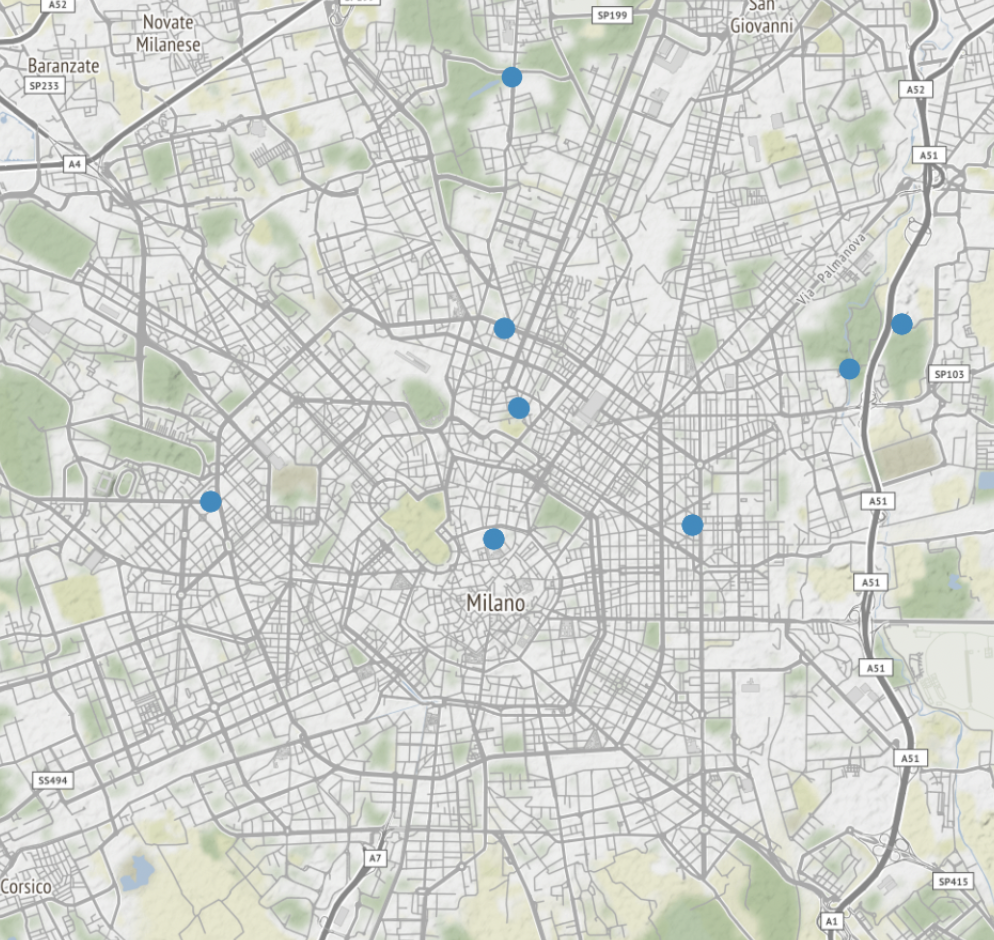
\includegraphics[width=\linewidth]{../src/meteo/centraline_ansa.png}
    \caption{Centraline Ansa a Milano}
    \label{fig:centraline-ansa}
\end{figure}

\todo{aggiungere centraline ansa mancanti}

Inoltre, per mancanza di dati precisi sul giorno degli incidenti, avere un'informazione così 
precisa sul meteo è superfluo.
Si è dunque optato per un dataset contenente temperature, umidità, e velocità del vento, 
trovato sul sito Zenodo
\footnote{\url{https://zenodo.org/record/3992354}}.

Il dataset contiene i campi specificati, misurati ogni ora, a partire dal 2008, fino al 2018.

\section{Dati riguardanti trasporti pubblici}
I dati riguardanti i trasporti pubblici trovati hanno due provenienze, i primi sono 
dati riferiti alle linee ATM, scaricati sul sito del comune di milano
\footnote{\url{https://dati.comune.milano.it/dataset/ds532-atm-composizione-percorsi-linee-di-superficie-urbane}}.
Dallo stesso sito proviene anche il dataset riguardante gli autobus turistici, che 
contiene in particolare le aree di sosta di questi ultimi
\footnote{\url{https://dati.comune.milano.it/dataset/ds740_sosta_bus_gt_turistici}}.

\section{Dati riguardanti autostrade e manto stradale}

Il primo dataset individuato, riguardante il manto  stradale, è stato quello di ANAS
\footnote{\url{http://dati.mit.gov.it/catalog/dataset/grafo-stradale-anas}}, 
tuttavia questo consisteva in un file molto grande.

Si è dunque tentato di utilizzare la mappa presente sul geoportale del comune di Milano
\footnote{\url{https://geoportale.comune.milano.it/}}, 
contenente anch'esso troppe strade in quanto traccia l'intero manto stradale del comune.

Entrambi questi dataset non risolvevano il problema del dataset mancante sul pavè.

Come ultima risorsa, si è deciso di tracciare alcune mappe in geojson utilizzando Geojson.io
\footnote{\url{https://geojson.io/}}, in particolare nella zona di Milano, per le principali 
autostrade, tangenziali e strade statali. 
Allo stesso modo, Geojson.io è stato utile a tracciare alcune aree in centro a Milano, per confrontare 
gli incidenti su pavè agli incidenti su asfalto.

\section{Dati riguardanti l'area C}

Oltre a utilizzare i dati riguardo agli accessi all'area C, si è fatto uso anche di una mappa 
raffigurante i varchi di entrata e i limiti del centro storico, 
proveniente dal sito del comune di Milano
\footnote{\url{https://www.comune.milano.it/aree-tematiche/mobilita/area-c}}.

\todo{lelepado: devo metterla questa? è solamente un'immagine}

\section{Dati riguardanti il turismo}

I dati sul turismo in Italia, sono stati presi dall'archivio istat sul tema
\footnote{\url{https://www.istat.it/it/archivio/16777}}.

I dati originali sono in formato xls, contenente informazioni a partire dal 1995 fino al 2019, 
sia regione per regione, sia divise per nord, centro e sud.
Sono anche presenti più tabelle, ognuna rafficurante un particolare indicatore, 
come produttività del lavoro, turismo nei mesi non estivi, tasso di turisticità e valore aggiunto del turismo.

Per realizzare la stima, sono stati necessari i dati regione per regione, 
a partire dal 2010 fino al 2018, convertiti in formato csv, si sono scelti gli indicatori di 
turismo nei mesi non estivi, e tasso di turisticità. 

\section{Immagini del traffico}

Le immagini raffiguranti il traffico in tempo reale sono prese da Google Maps
\footnote{\url{https://www.google.com/maps/}}, 
tuttavia questi snapshot contengono molti punti di interesse che coprono informazioni importanti, 
come i nomi delle strade.

Per rimuovere i punti di interesse, si sono utilizzate le API di google maps, 
tramite il sito Jsfiddle
\footnote{https://jsfiddle.net/}.

Si sono infine realizzati degli screenshot della zona dei Navigli e dell'incrocio tra viale 
Bianca Maria e viale 22 Marzo.

%%%%%%%%%%%%%%%%%%%%%%%%%%%%%%%%%%%%%%%%%%%%%%%%%%%%%%
\section{Dati mancanti}

\subsection{Dati riguardanti pavè}
Non sembra che esista un dataset contenente la composizione del manto stradale di Milano.
I dati in questione sono stati cercati sui principali siti di opendata
\footnote{\url{https://dati.comune.milano.it/dataset}}
\footnote{\url{https://www.dati.lombardia.it/}}
\footnote{\url{https://www.dati.gov.it/}}
tramite parole chiave come \textit{strada}, \textit{manto stradale}, \textit{pave}, 
\textit{composizione strada}.

Una possibile risorsa trovata è una mappa utilizzata in un articolo del blog urbanfile
\footnote{\url{https://blog.urbanfile.org/2018/05/02/milano-arredo-urbano-il-pave-risorsa-da-preservare-o-problema-da-eliminare/}}.
Dopo una rapida consultazione tuttavia, non risulta esserci alcun dataset contenente informazioni 
riguardanti il pavè a Milano, infatti la cartina è stata realizzata tramite conoscenza personale dell'autore dell'articolo.

Il dataset che potrebbe avvicinarsi di più ad ottenere le informazioni cercate potrebbe essere 
quello riguardante i percorsi dei trasporti tranviari. Basandosi su queste informazioni, e assumendo che 
la maggior parte delle linee dei tram a Milano sono pavimentate in pavè, è possibile ottenere un dataset con taglia discreta.

\'E possibile confrontare il dataset ottenuto con la mappa di Urbanfile e, 
per quanto alcune linee coincidano, non si è trovata somiglianza sufficiente 
per giustificare la stima.

Come ultima spiaggia, si è deciso di tracciare una mappa utilizzando Geojson.io
\footnote{\url{https://geojson.io/}}, come già fatto per le autostrade a Milano, 
basandosi sulla cartina di Urbanfile. 

\subsection{Dati riguardanti traffico stradale}
Per quanto riguarda i dati sul traffico stradale, anche in questo caso non è stato trovato un 
dataset, sia nei siti di cui si è parlato in precedenza, sia su quello di autostrade
\footnote{\url{http://www.autostrade.it/it/home}}.

Il primo tentativo, per avere una stima del traffico è stato la realizzazione di uno script per 
fare scraping da Google Maps. Quest'ultimo infatti mostra sia il traffico in tempo reale, sia 
il traffico stimato a una determinata ora. Tuttavia, leggendo nella documentazione, si è scoperto che 
non è possibile ottenere dati sul traffico stimato, per mancanza di API. 
Per quanto fosse stato possibile realizzare comunque uno script per effettuare scraping della 
quantità di traffico nelle strade, si è optato per la ricerca di un altro dataset.

Dunque si è deciso di utilizzare i dati riguardanti gli ingressi in area C a Milano, 
trovati sul sito del comune di Milano
\footnote{\url{https://dati.comune.milano.it/dataset}}, 
nonostante non permetta una stima perfetta.

Sul sito del comune di Milano sono disponibili varie tipologie di file, 
ceh suddividono i dati in base a, per esempio, orario, mese, località. 
Tra questi si è utilizzata la tipologia contenente orari e data dell'accesso.

Un'altro dataset utilizzato per stimare il numero di automobili, è quello contenente il numero di 
patentati per regione, trovato nel sito del Ministero dei Trasporti
\footnote{\url{dati.mit.gov.it/catalog/dataset/patenti}}.
I dati, riguardanti i patentati fino al 2019, sono divisi in file per regione e contengono anche 
informazioni riguardanti la provincia e data di conseguimento della patente, 
oltre al tipo di ceritificato ottenuto.


%%%%%%%%%%%%%%%%%%%%%%%%%%%%%%%%%%%%%%%%%%%%%%%%%%%%%%
\chapter{Dati Geolocalizzati}

\section{Incidenti}

Controllando i dati trovati, in particolare come questi siano distributi, 
si nota subito dalla mappa \ref{fig:geo-incidenti} che gli incidenti a Milano sono per buona parte uniformemente sparsi in tutta la città, 
con più alta concentrazione in alcuni punti di interesse, come Piazzale Loreto, Zona Navigli 
e Monumentale, e Corso Ventidue Marzo.

\begin{figure}
    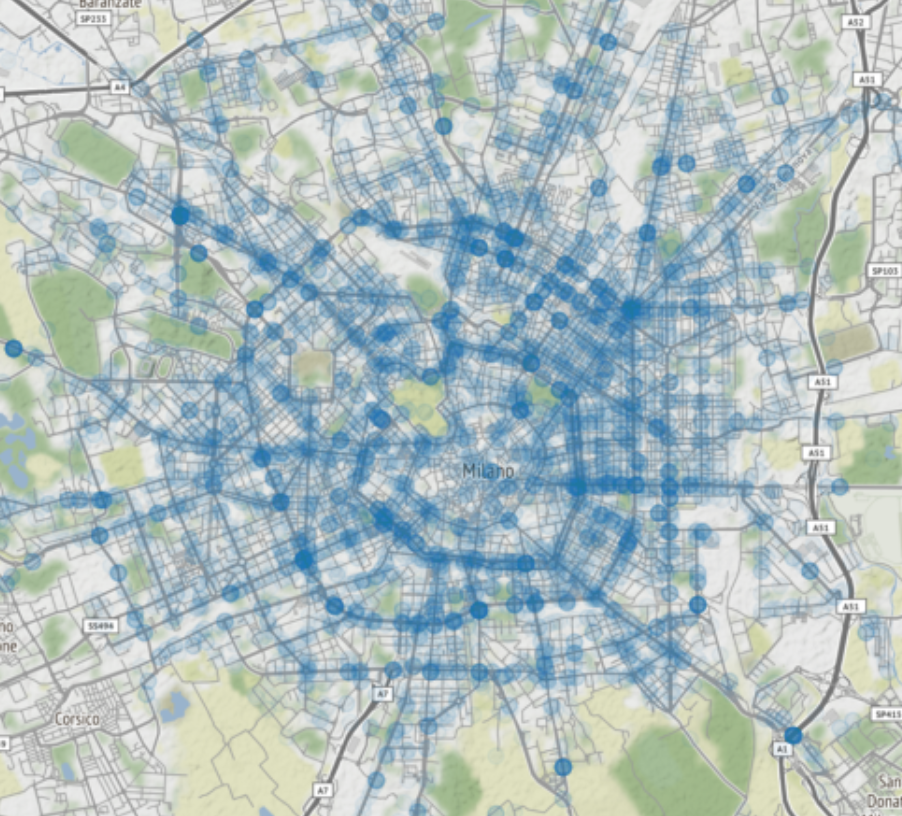
\includegraphics[width=\linewidth]{../src/incidenti/geo_incidenti.png}
    \caption{Distribuzione di incidenti a Milano}
    \label{fig:geo-incidenti}
\end{figure}

Sarebbe interessante sapere se esistono zone con maggiore concentrazione di incidenti rispetto 
alla media, e sarebbe interessante ottenere un indice numerico della pericolosità di una 
determinata zona.\\
Nella figura \ref{fig:heatmap-municipi}, si è divisa la città di Milano in base al comune, ed è 
chiaramente visibile che il centro ha la maggior parte degli incidenti.

\begin{figure}
    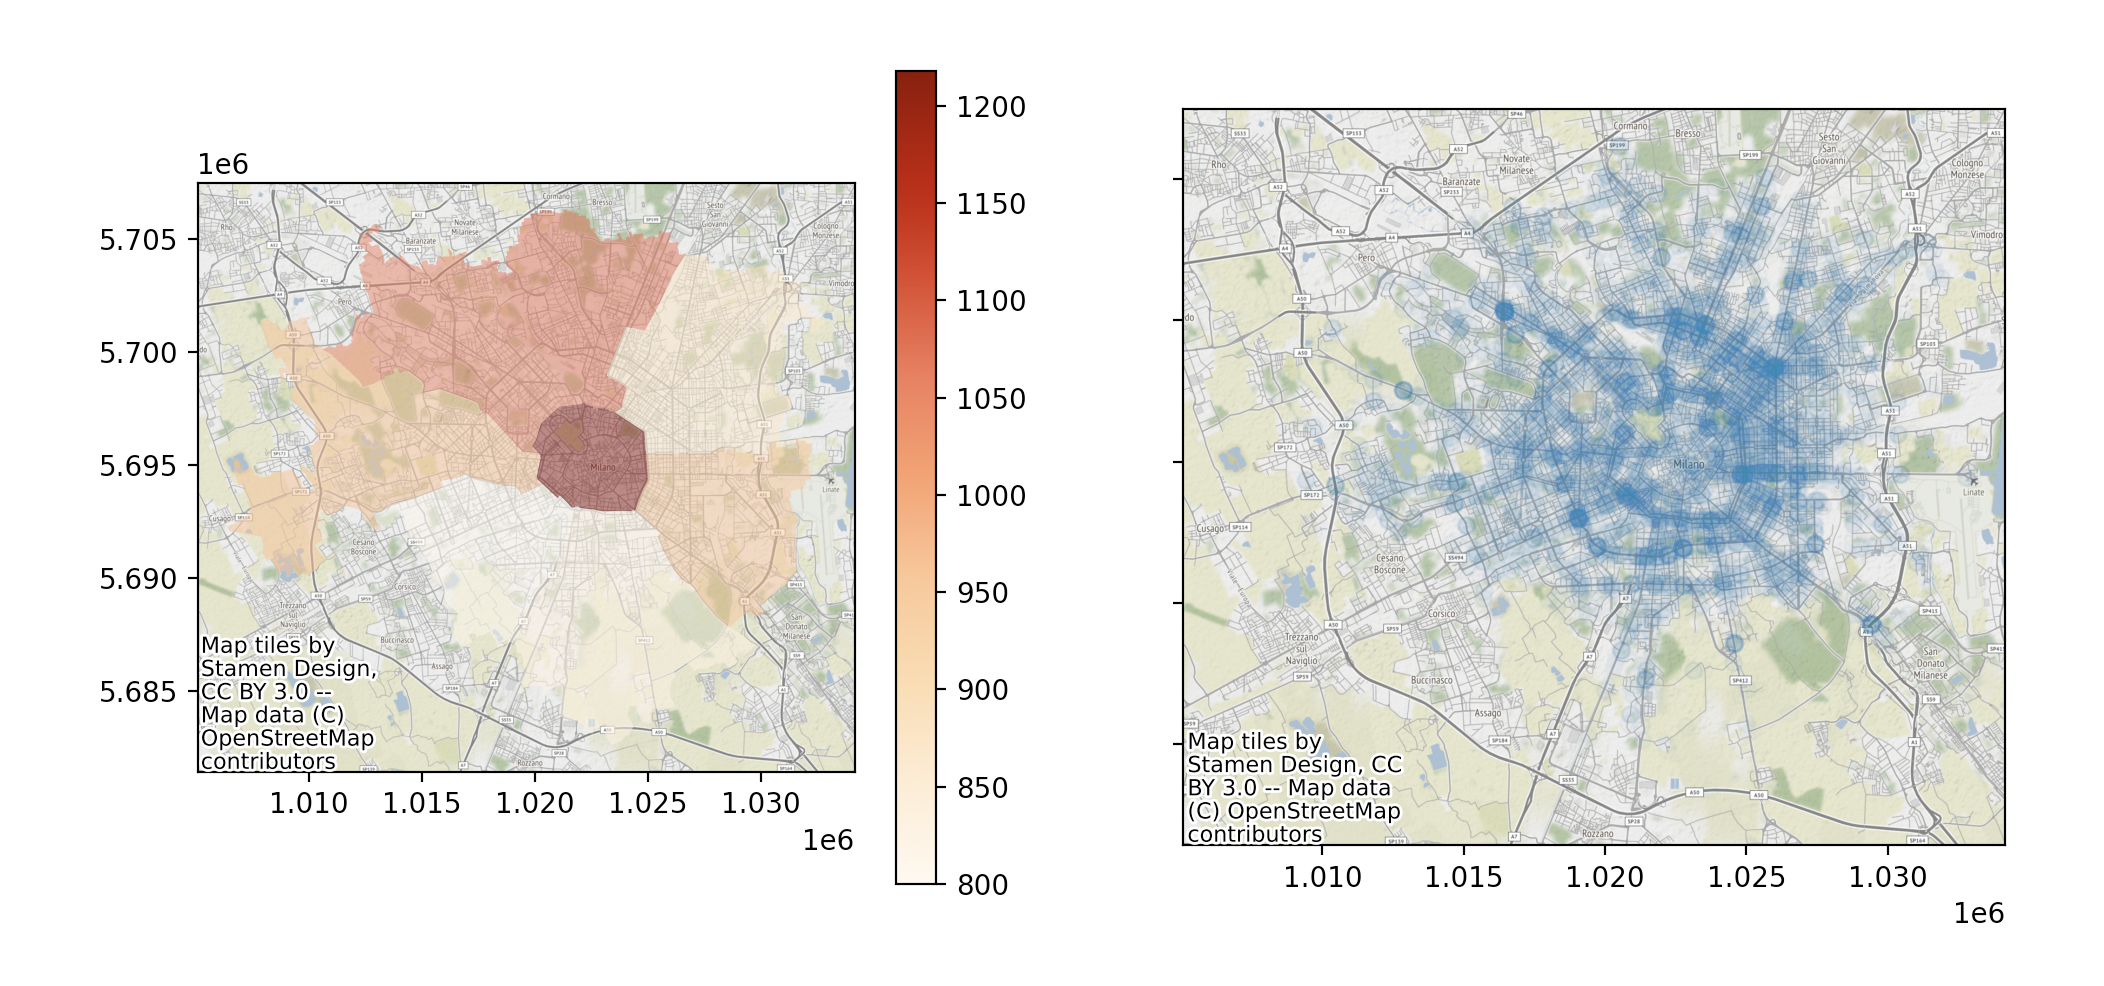
\includegraphics[width=\linewidth]{../src/municipi_milano/incidenti_municipio.png}
    \caption{Incidenti a Milano per municipio}
    \label{fig:heatmap-municipi}
\end{figure}

Tuttavia, non tutte le zone hanno la stessa superficie. Avendo a disposizione l'area delle varie zone, 
è possibile calcolare la media di incidenti al chilometro quadrato per zona.

\begin{lstlisting}    
    inc = gp.GeoSeries(df).sort_index()

    area = pd.Series(data['AREA'], index=data['MUNICIPIO'])
    incidenti = pd.Series(inc, index=inc.index)

    incidenti_per_zona = (incidenti / area) * 1000000 # trasformazione in chilometri quadri
\end{lstlisting}

\begin{center}
    \def\arraystretch{1.5}%  
    \begin{tabular}{ |c|c| } 
    \hline
    Numero della zona & Nome della zona \\ 
    \hline
    \rowcolor{TableGray}
    1   &   Centro Storico\\
    2   &   Greco, Padova\\
    \rowcolor{TableGray}
    3   &   Venezia, Città Studi\\
    4   &   Vittoria, Vigentina \\
    \rowcolor{TableGray}
    5   &   Ticinese, Gratosoglio\\
    6   &   Inganni, Barona\\
    \rowcolor{TableGray}
    7   &   Baggio, Forze Armate\\
    8   &   Gallaratese, Sempione\\
    \rowcolor{TableGray}
    9   &   Niguarda, Dergano\\
    \hline
    \end{tabular}
\end{center}

\begin{figure}
    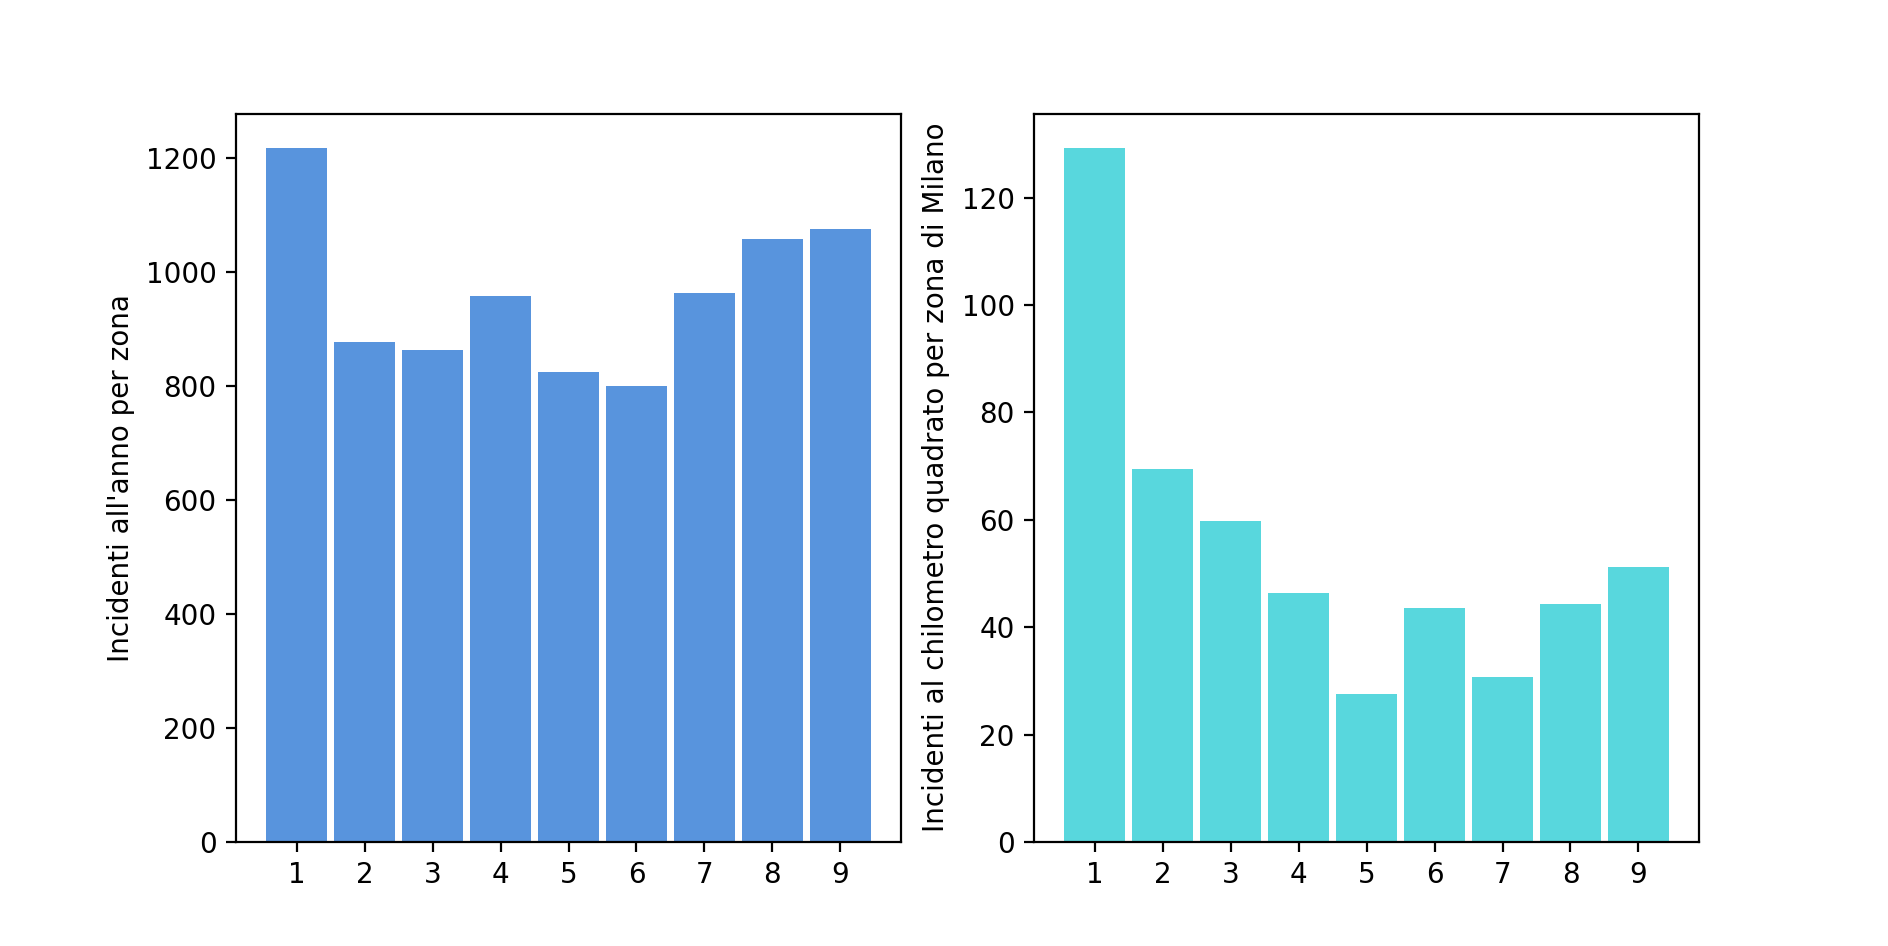
\includegraphics[width=\linewidth]{../src/municipi_milano/incidenti_superf.png}
    \caption{Incidenti a Milano per zona e in base alla superficie della zona}
    \label{fig:incidenti-chilometro}
\end{figure}

Nella figura \ref{fig:incidenti-chilometro} spicca, sia nel grafo di sinistra che in quello di destra, 
la zona 1, cioè quella del centro, vista la superficie minore rispetto agli altri municipi.

Una volta creata una tendenza della zona, è possibile confrontare i risultati ottenuti con i numeri 
di incidenti in zone più precise, per esempio attorno a piazzale Loreto.

\begin{figure}
    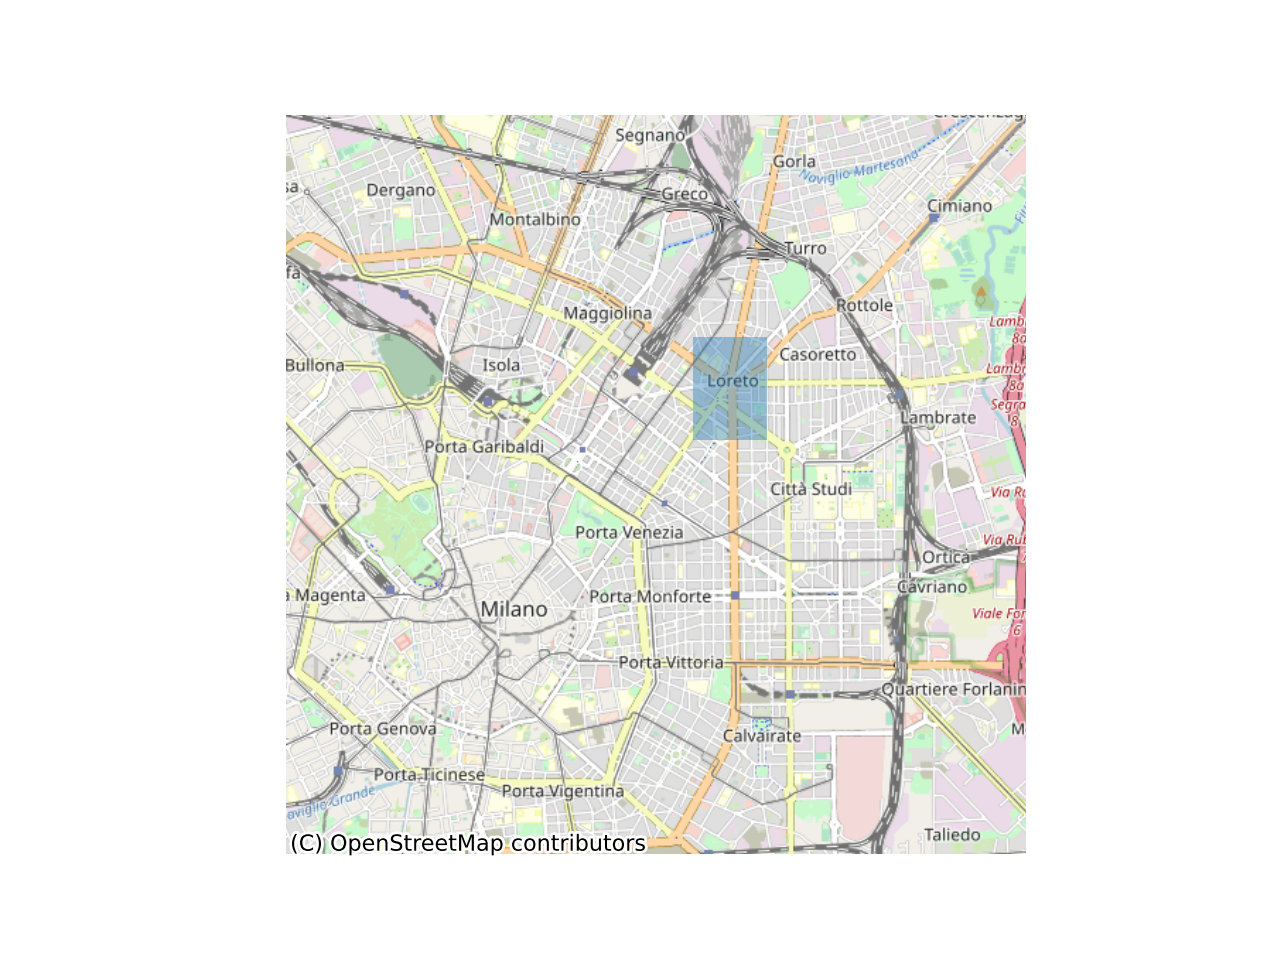
\includegraphics[width=\linewidth]{../src/municipi_milano/zona_loreto.png}
    \caption{Zona presa in considerazione per piazzale Loreto}
    \label{fig:zona-loreto}
\end{figure}

\begin{lstlisting}
    loreto = geometry.Polygon([p1, p2, p4, p3])

    loreto_incidenti = 0
    for point in incidenti['geometry']: 
        point = geometry.Point(point)

        if loreto.contains(point): 
            loreto_incidenti += 1

    area_loreto = loreto.area * data['AREA'].iloc[0] / geometry.Polygon(data['geometry'].iloc[0]).area
    area_loreto_inc = loreto_incidenti * 1000000 / area_loreto
\end{lstlisting}

Il numero di incidenti che risultano, nell'area considerata in figura \ref{fig:zona-loreto}, 
sono 231.06, considerando che il massimo ottenuto per zona, il centro storico arriva attorno a 120, 
è possibile assumere che piazzale loreto sia una zona ad alta incidentalità.

Andrebbe anche spiegato il fatto che il centro storico sia una delle zone con maggiore incidentalità, 
non dovrebbe essere abbassata della presenza dell'area C?

\begin{figure}
    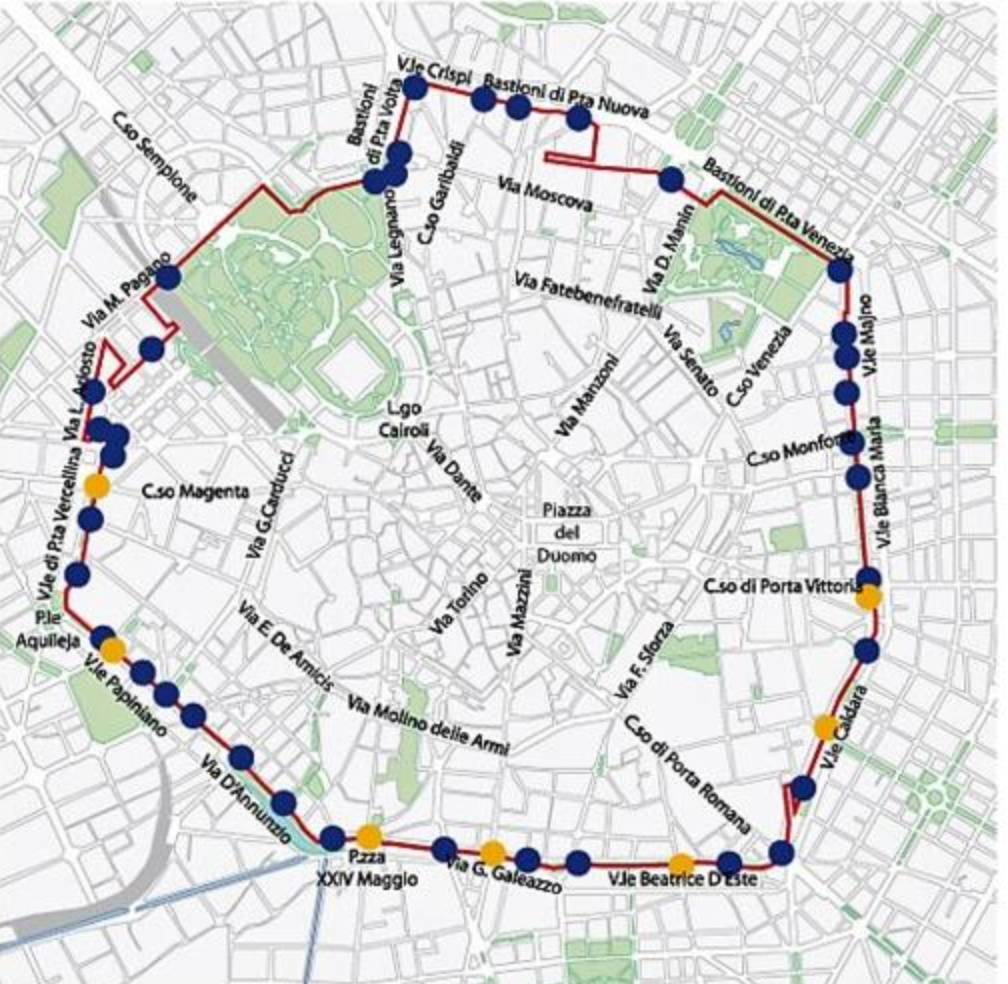
\includegraphics[width=0.48\linewidth]{../dataset/area_c/perimetro_area_c.png}
    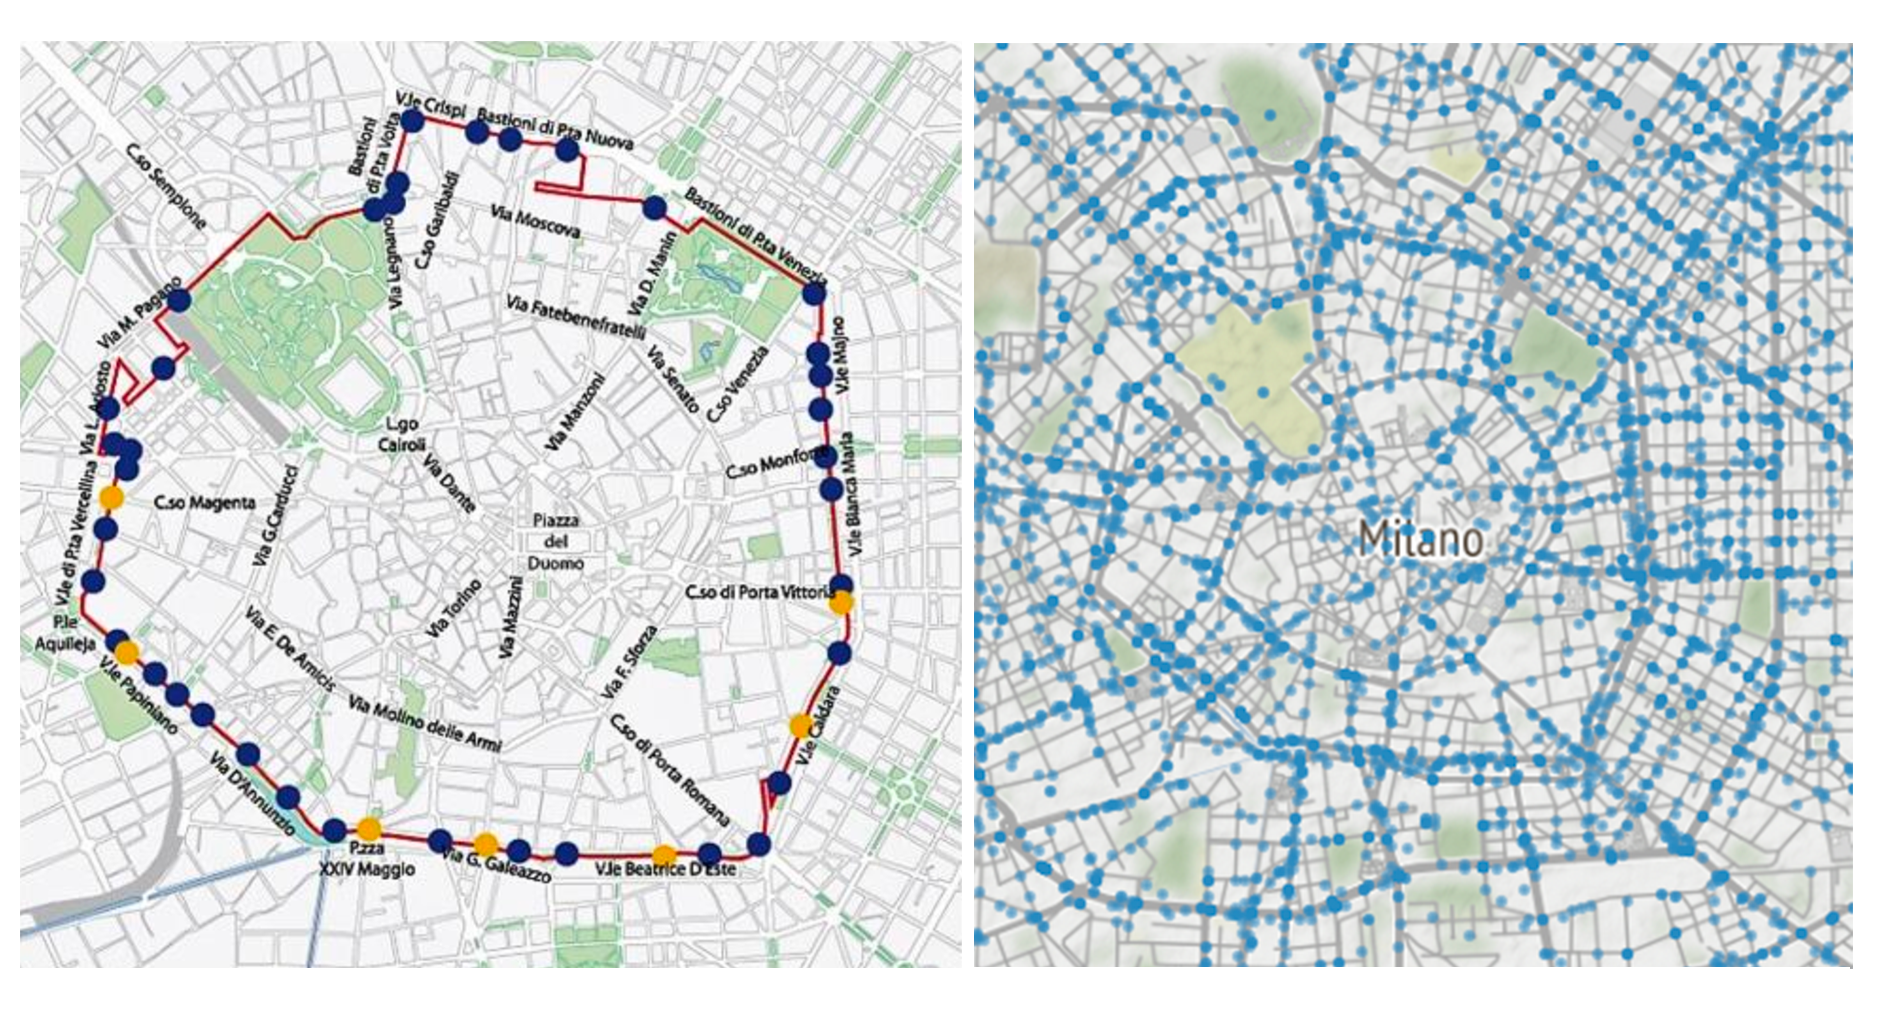
\includegraphics[width=0.52\linewidth]{../src/area_c/area_c_incidenti.png}
    \caption{Perimetro dell'area C e incidenti nella stessa zona}
    \label{fig:perimetro-area-c}
\end{figure}

Dopo più attenta osservazione del perimetro dell'area C, visibile in figura \ref{fig:perimetro-area-c}, 
si nota che la maggior parte degli incidenti avvengono sulla circonvallazione interna, 
situata fuori dall'area C, che è compresa nell'area 0 di Milano nella mappa \ref{fig:heatmap-municipi}.

Se si prende in considerazione solamente l'area C, il numero di incidenti scende a $46.83$ per chilometro quadrato.

\begin{lstlisting}
    area_c = geometry.Polygon(gp.read_file("dataset/area_c/area_c.geojson").to_crs(epsg=3857)['geometry'].iloc[0])

    inc = 0
    for point in incidenti['geometry']: 
        if area_c.contains(geometry.Point(point)): 
            inc += 1
\end{lstlisting}

%\clearpage
\section{Incidenti e Linee dei Trasporti Pubblici}

Il dataset dei tragitti dei trasporti pubblici copre molta più superficie rispetto a 
quello degli incidenti.
Dopo aver eliminato alcune linee di autobus che risultavano troppo in periferia, 
si ottiene la figura \ref{fig:geo-trasporti}: 

\begin{figure}
    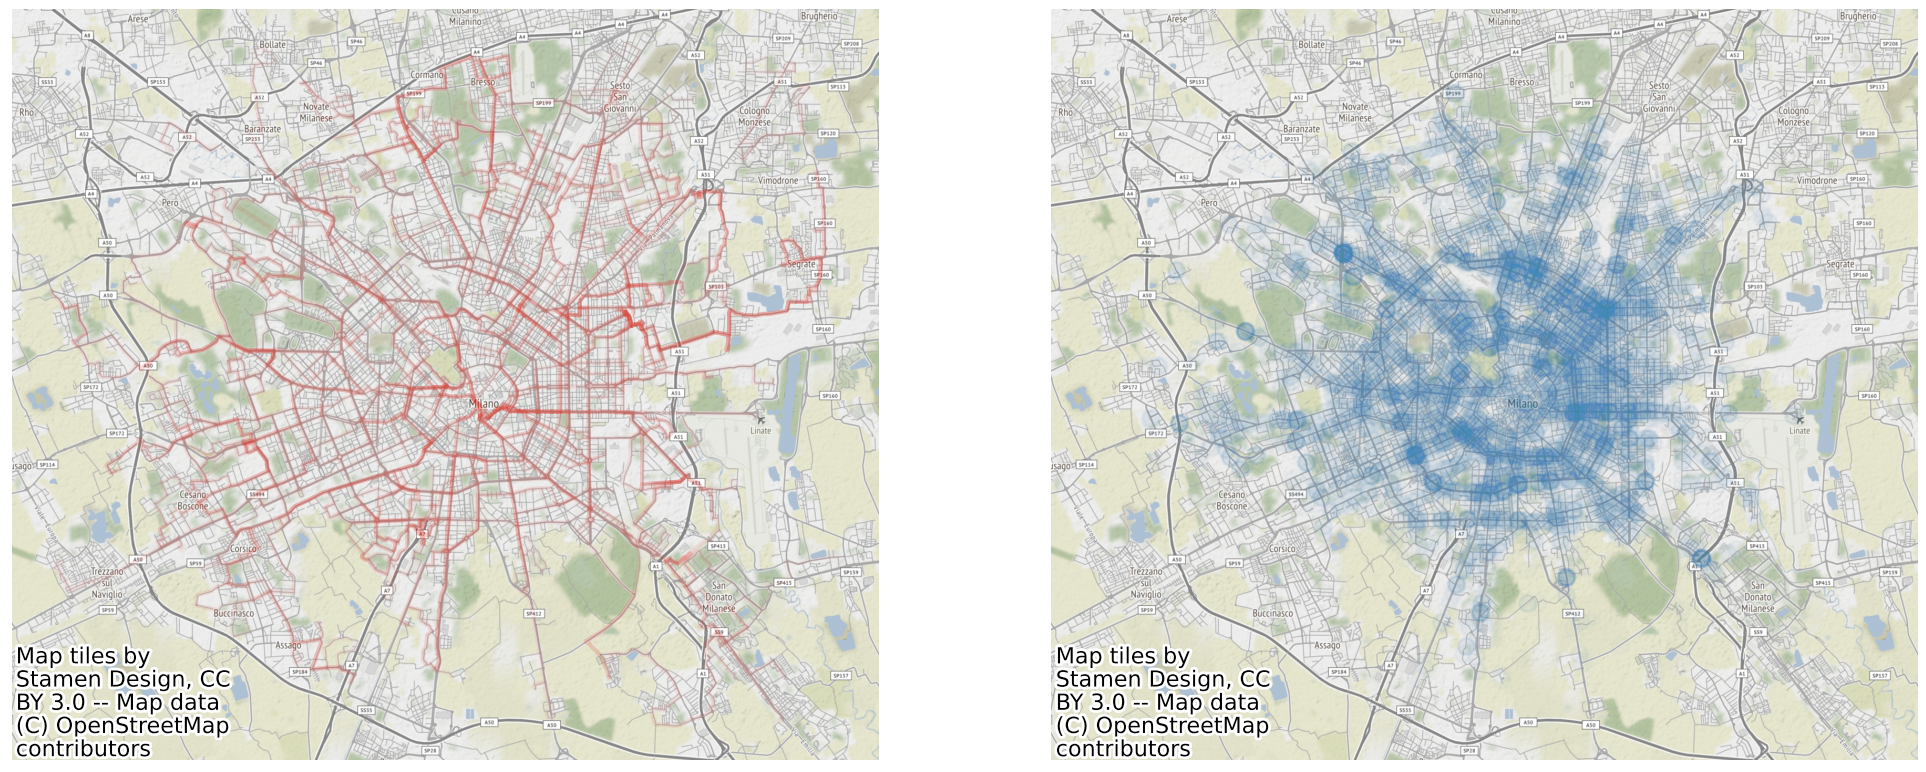
\includegraphics[width=\linewidth]{../src/atm/linee_atm.png}
    \caption{Linee Autobus e Tram a Milano}
    \label{fig:geo-trasporti}
\end{figure}

Nonstante la rimozione di parte dei tragitti, i trasporti pubblici coprono 
la maggior parte della città.
Se a questi ultimi vengono sovrapposti i dati sugli incidenti, 
si può notare che la maggior parte dei luoghi con alta concentrazione di incidenti sono 
attraversati da linee di autobus. Nel caso di Corso Ventidue Marzo, si ha anche una linea di tram.

Dalla sovrapposizione delle mappe, si può notare anche che, alcune strade con alta incidentalità 
sono parallele a linee di autobus. 
Un esempio è quello di zona Navigli, in figura \ref{fig:navigli}, dove le vie interessate sono:
Viale Gian Galeazzo e Viale Beatrice D'Este, parallele a Viale Col di Lana e Viale Bligny.
La stessa cosa si pu\'o notare su Viale Gabriele D'Annunzio e Viale Gorizia e Coni Zugna.

\begin{figure}
    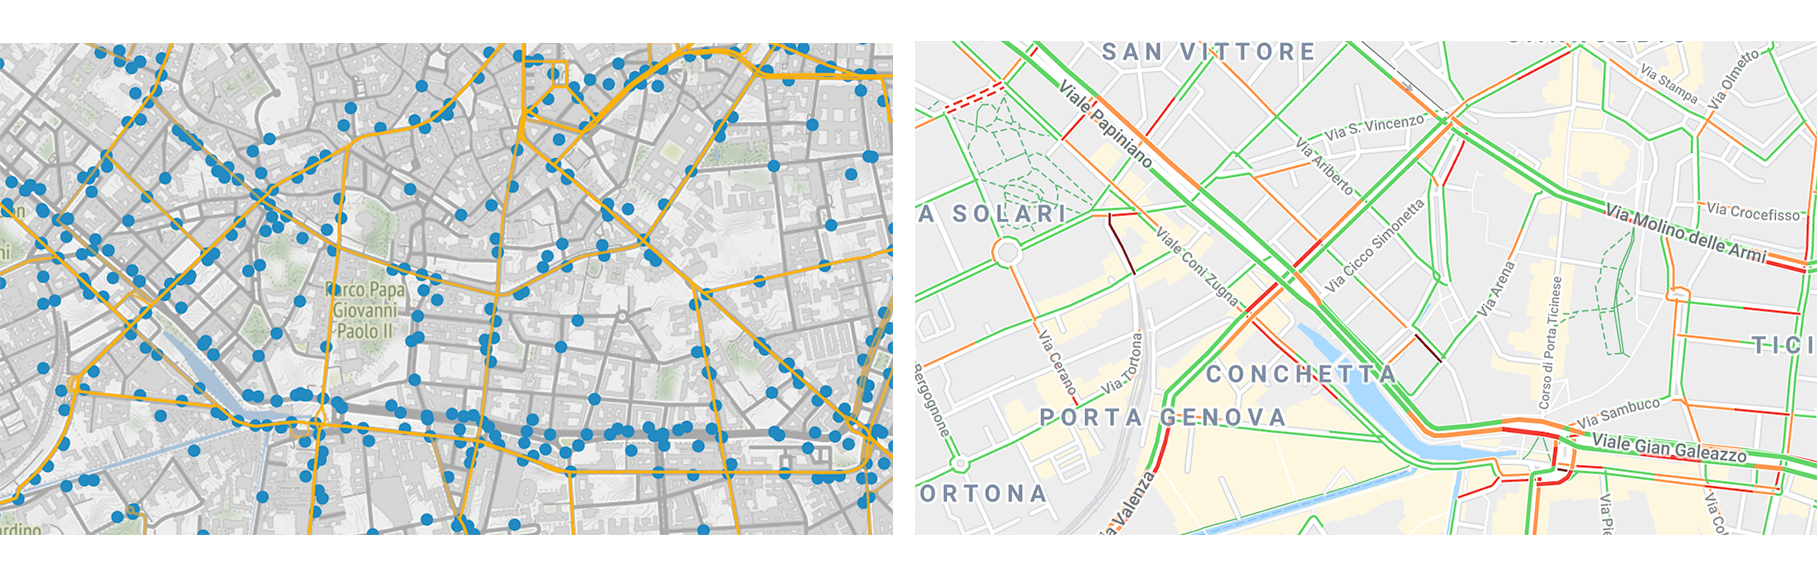
\includegraphics[width=0.51\linewidth]{../src/atm/navigli.png}
    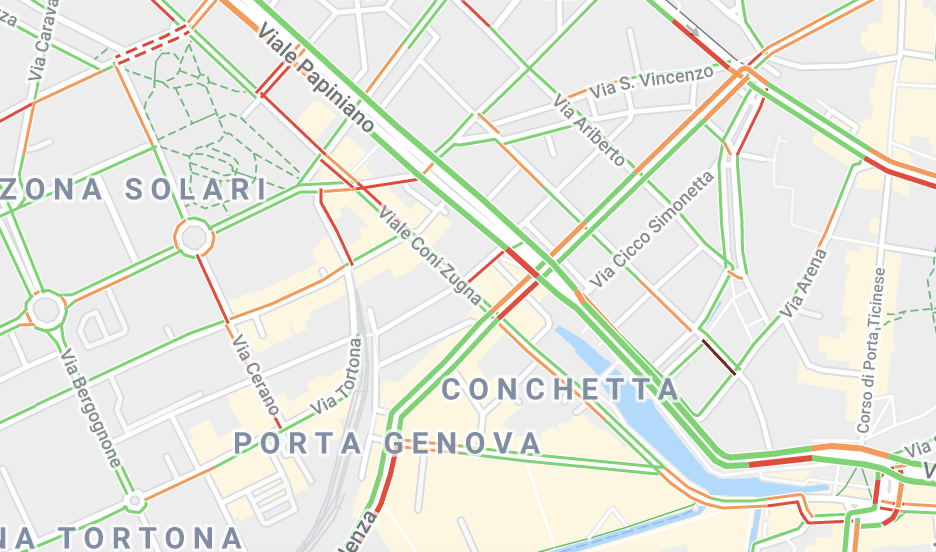
\includegraphics[width=0.49\linewidth]{../src/codice_per_dati/googleMaps/navigli.png}
    \caption{Linee dei trasporti pubblici e condizioni di traffico nella zona Navigli}
    \label{fig:navigli}
\end{figure}

Anche vicino a corso Ventidue Marzo, nella mappa \ref{fig:22-marzo} si può 
notare lo stesso fenomeno, tra Viale Bianca Maria e Viale Premuda.

\begin{figure}
    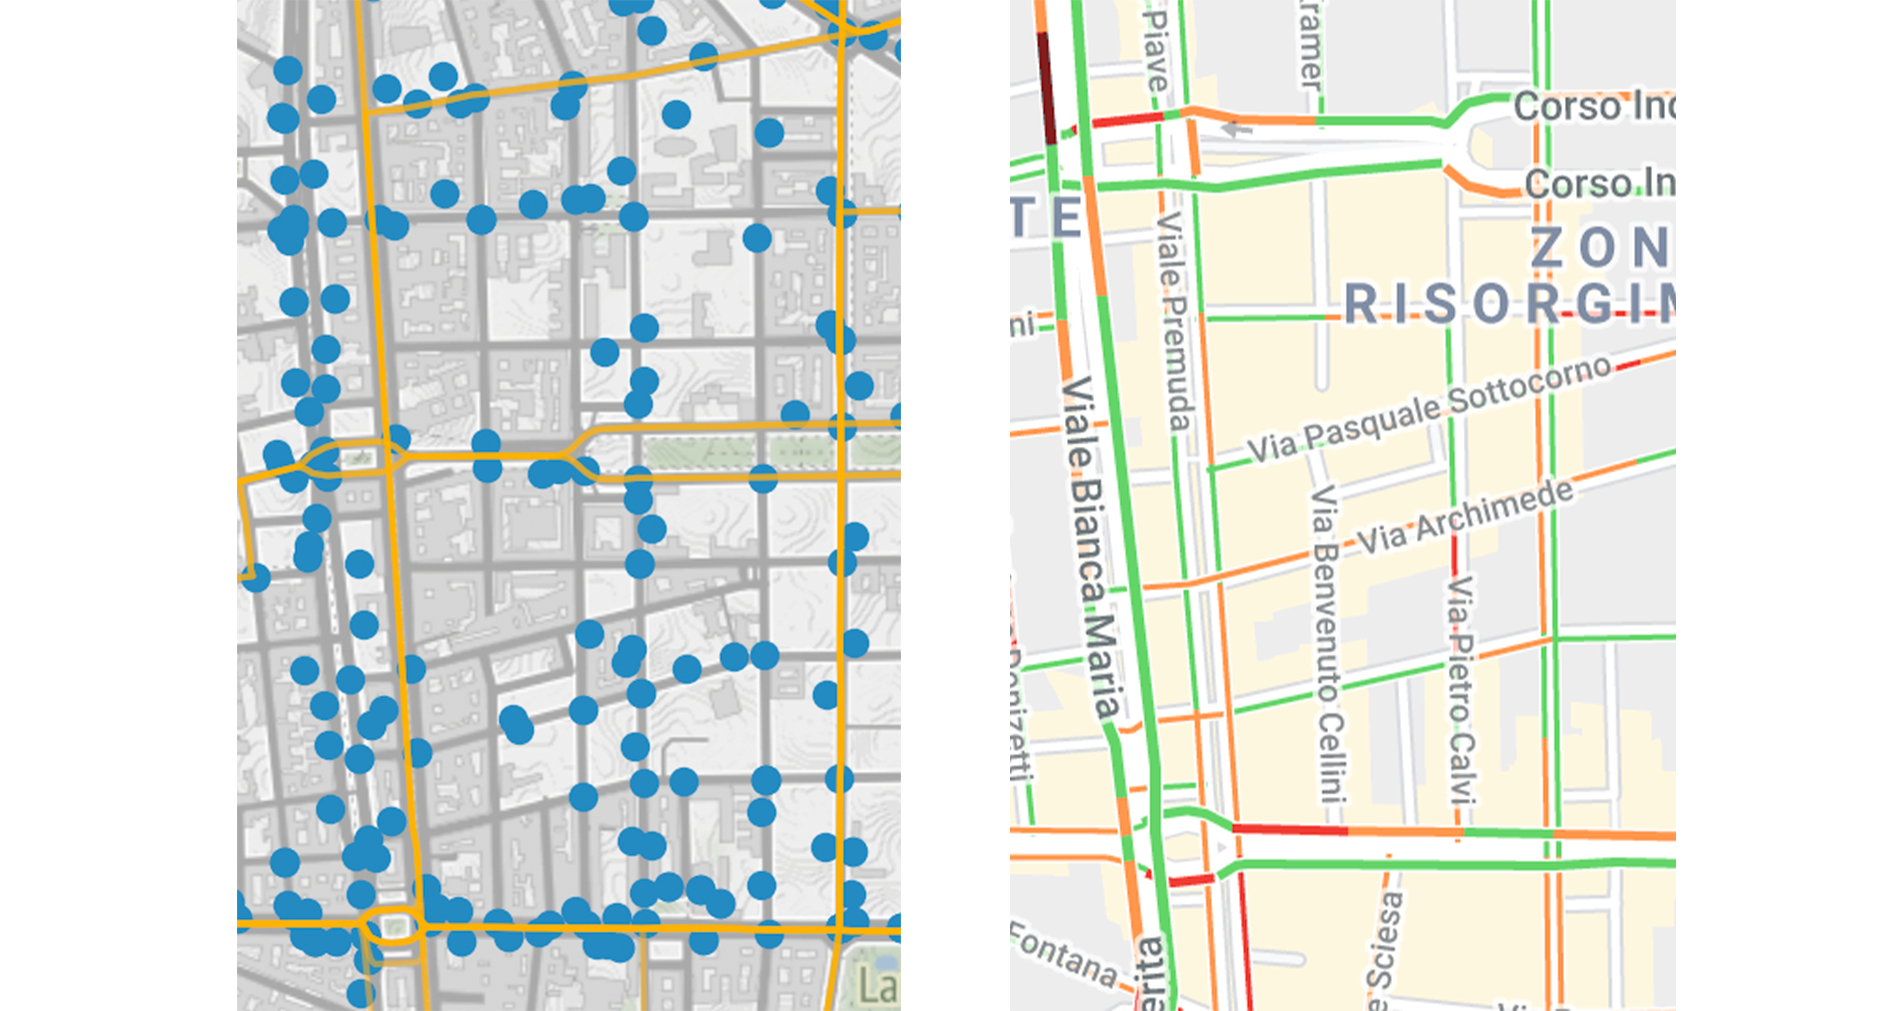
\includegraphics[width=0.45\linewidth]{../src/atm/22_marzo.png}
    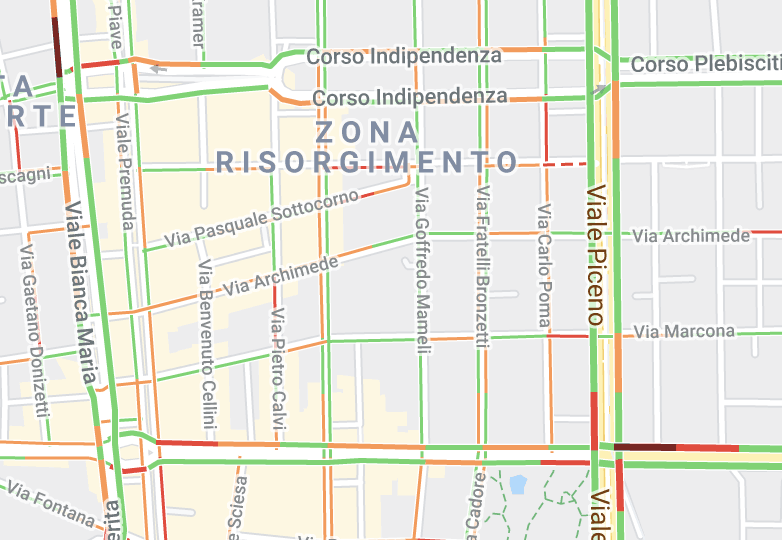
\includegraphics[width=0.55\linewidth]{../src/codice_per_dati/googleMaps/22_marzo.png}
    \caption{Linee dei trasporti pubblici e condizioni traffico vicino a Corso 22 Marzo}
    \label{fig:22-marzo}
\end{figure}

Le immagini del traffico sono state realizzate tramite le API di Google Maps:  

\begin{lstlisting}
const styles = {
  hide: [
    {
      featureType: "poi", // poi indica i punti di interesse
      stylers: [{ visibility: "off" }],
    }
\end{lstlisting}

Per confutare l'ipotesi, si sono usati i dati ricavati in precedenza, 
di incindenti per chilometro per zona di Milano. 
Nella zona dei navigli, si è poi presa in considerazione la sezione \ref{fig:zona-navigli-rect}, 
perchè sono presenti molti incidenti in viale Papiniano e viale Beatrice d'Este, 
e un numero minore nella via parallela sottostante, in cui è anche presente 
una linea di trasporti pubblici.

\begin{figure}
    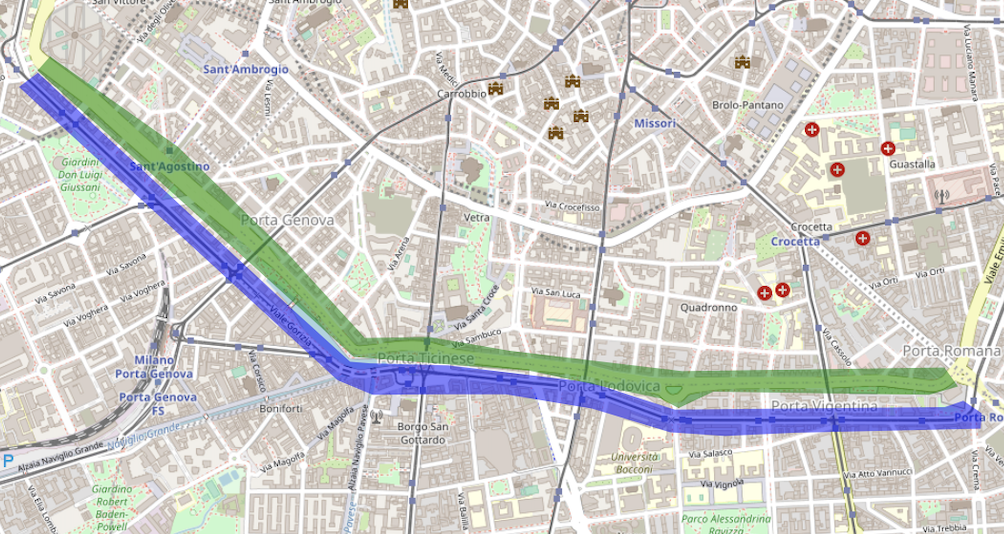
\includegraphics[width=\linewidth]{../src/atm/zona_navigli_rect.png}
    \caption{Sezioni di Milano prese in considerazione per contare gli incidenti ai navigli}
    \label{fig:zona-navigli-rect}
\end{figure}

\begin{lstlisting}
    data = gp.read_file("dataset/zone_milano/zone.geojson").to_crs(epsg=3857)
    autobus = data[data['name'] == "Navigli Autobus"]
    street = data[data['name'] == "Navigli Incidenti"]

    autobus_rect = geometry.Polygon(autobus['geometry'].iloc[0])
    street_rect = geometry.Polygon(street['geometry'].iloc[0])

    inc_a = 0
    inc_s = 0
    for point in incidenti['geometry']: 
        point = geometry.Point(point)

        if autobus_rect.contains(point): 
            inc_a += 1
        
        if street_rect.contains(point): 
            inc_s += 1
\end{lstlisting}

Il risultato, conferma che sono presenti $167.09$ incidenti per chilometro 
nel viale in cui sono presenti trasporti pubblici, che per quanto non sia nella media per la zona 
di appartenenza, è giustificabile in quanto si è presa in considerazione solo la strada, 
e $289.32$ nell'altra zona. Nel secondo caso il numero di incidenti è molto alto.

Non è detto che il maggior numero di incidenti sia causato dalla linea degli autobus, 
in particolare, va tenuta in considerazione la topologia delle due vie parallele.
La differenza principale tra viale Bligny e viale Beatrice d'Este è che, il primo è una via a due 
corsie per senso di marcia, mentre il secondo è un viale a due carreggiate
\footnote{Carreggiata: la parte della strada destinata allo scorrimento dei veicoli, 
delimitata da una striscia continua o da un paracarro} 
con sensi di marcia separati. 

Lo stesso procedimento è stato realizzato per corso 22 Marzo, le zone utilizzate sono 
raffigurate nel'immagine \ref{fig:zona-22marzo-rect}. 

\begin{figure}
    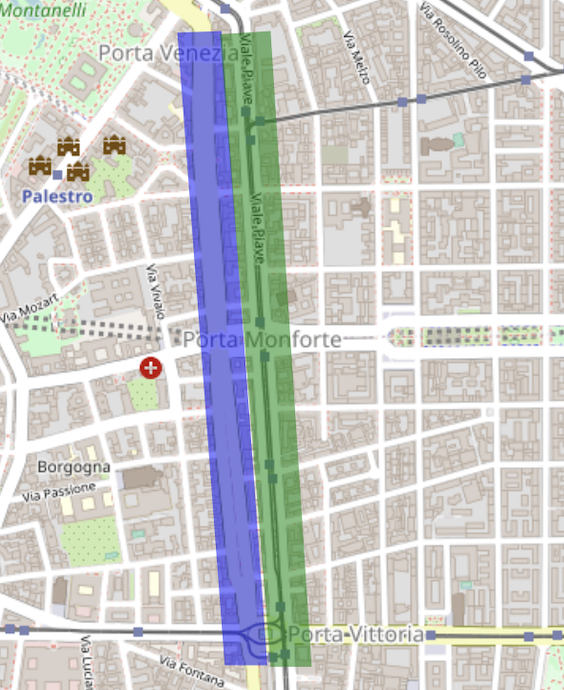
\includegraphics[width=\linewidth]{../src/atm/zona_22marzo_rect.png}
    \caption{Sezioni di Milano prese in considerazione per contare gli incidenti intorno a corso 22 Marzo}
    \label{fig:zona-22marzo-rect}
\end{figure}

In questo caso, per viale Bianca Maria, dove non è presente una linea di trasporti pubblici, 
il numero di incidenti è $254.31$, mentre per viale Premuda per cui passa una linea tranviaria, 
il numero scende a $93.96$.

Anche per questa zona, le due vie prese in considerazione sono molto diverse; 
viale Premuda è una via a due carreggiate separate, ognuna con una corsia e un solo senso di marcia, 
dove sono parcheggiate automobili su entambi i lati, e la velocità di marcia non deve essere particolarmente 
elevata.
D'altra parte viale Bianca Maria, pur avendo carreggiate separate, queste hanno due, e in alcuni punti tre, 
corsie ciascuna; con l'aumentare dello spazio, infine, inevitabilmente la velocità delle automobili aumenta.

\todo{ci sono vie con la tendenza opposta?}

%\clearpage
\subsection{Il pavè a Milano influisce in qualche modo sull'incidentalità?}

Spesso le linee di tram coincidono con strade in pavè, è vero per Milano? 
Tramite la mappa \ref{fig:tram-pave-milano} è possibile confrontarle: 

\begin{figure}
    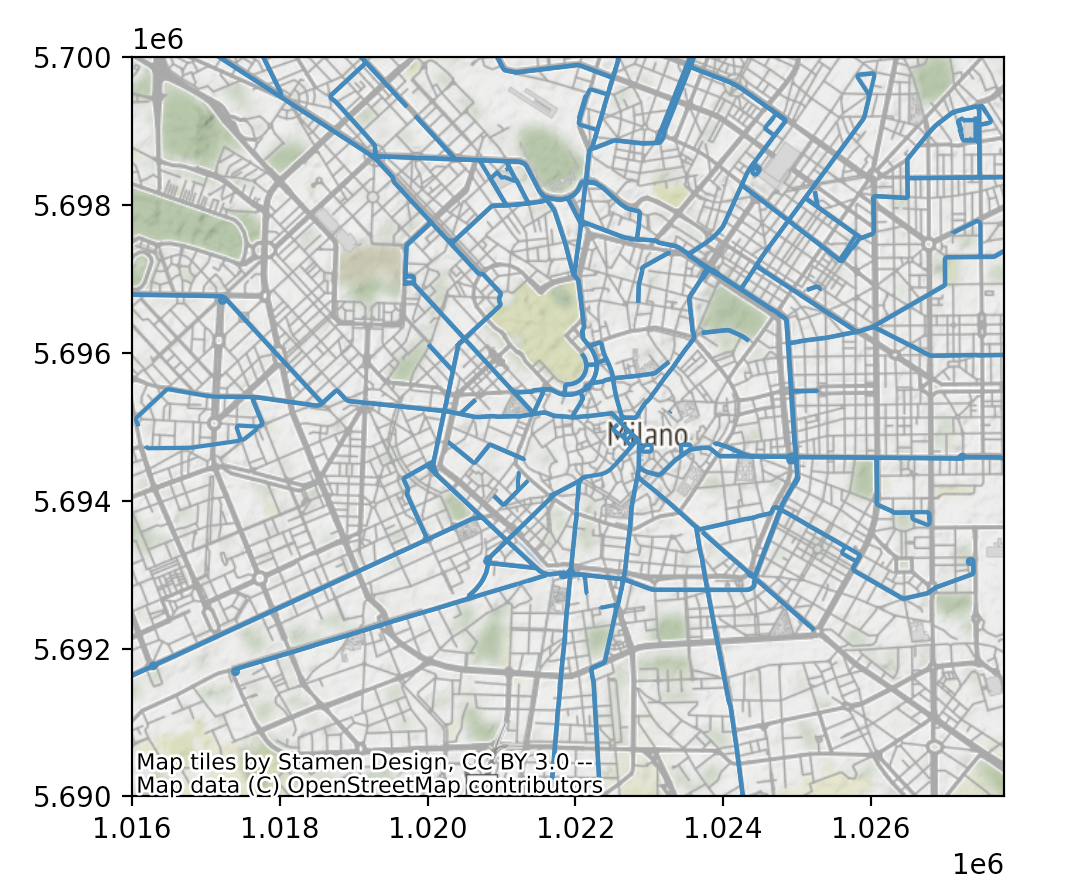
\includegraphics[width=0.48\linewidth]{../src/tram/tram.png}
    \includegraphics[width=0.52\linewidth]{../dataset/pave/Cartina_Milano_Strade_Pavimentazione_Pavé_2.jpg}
    \caption{Cartina con strade in pavè e linee tranviarie a Milano}
    \label{fig:tram-pave-milano}
\end{figure}

Si notano alcune somiglianze, come per esempio viale Sabotino e via Alessandro Mazoni, 
tuttavia la maggior parte delle linee tramviarie segnate passano su asfalto.
Inoltre, in alcuni viali, come viale Premuda, i tram hanno una carreggiata separata, 
che probabilmente ha influenza ancora minore.

Per creare una stima, si sono convertite le vie principali della cartina trovata 
in geojson, il risultato è visibile nella mappa \ref{fig:mappa-pave}.

\begin{figure}
    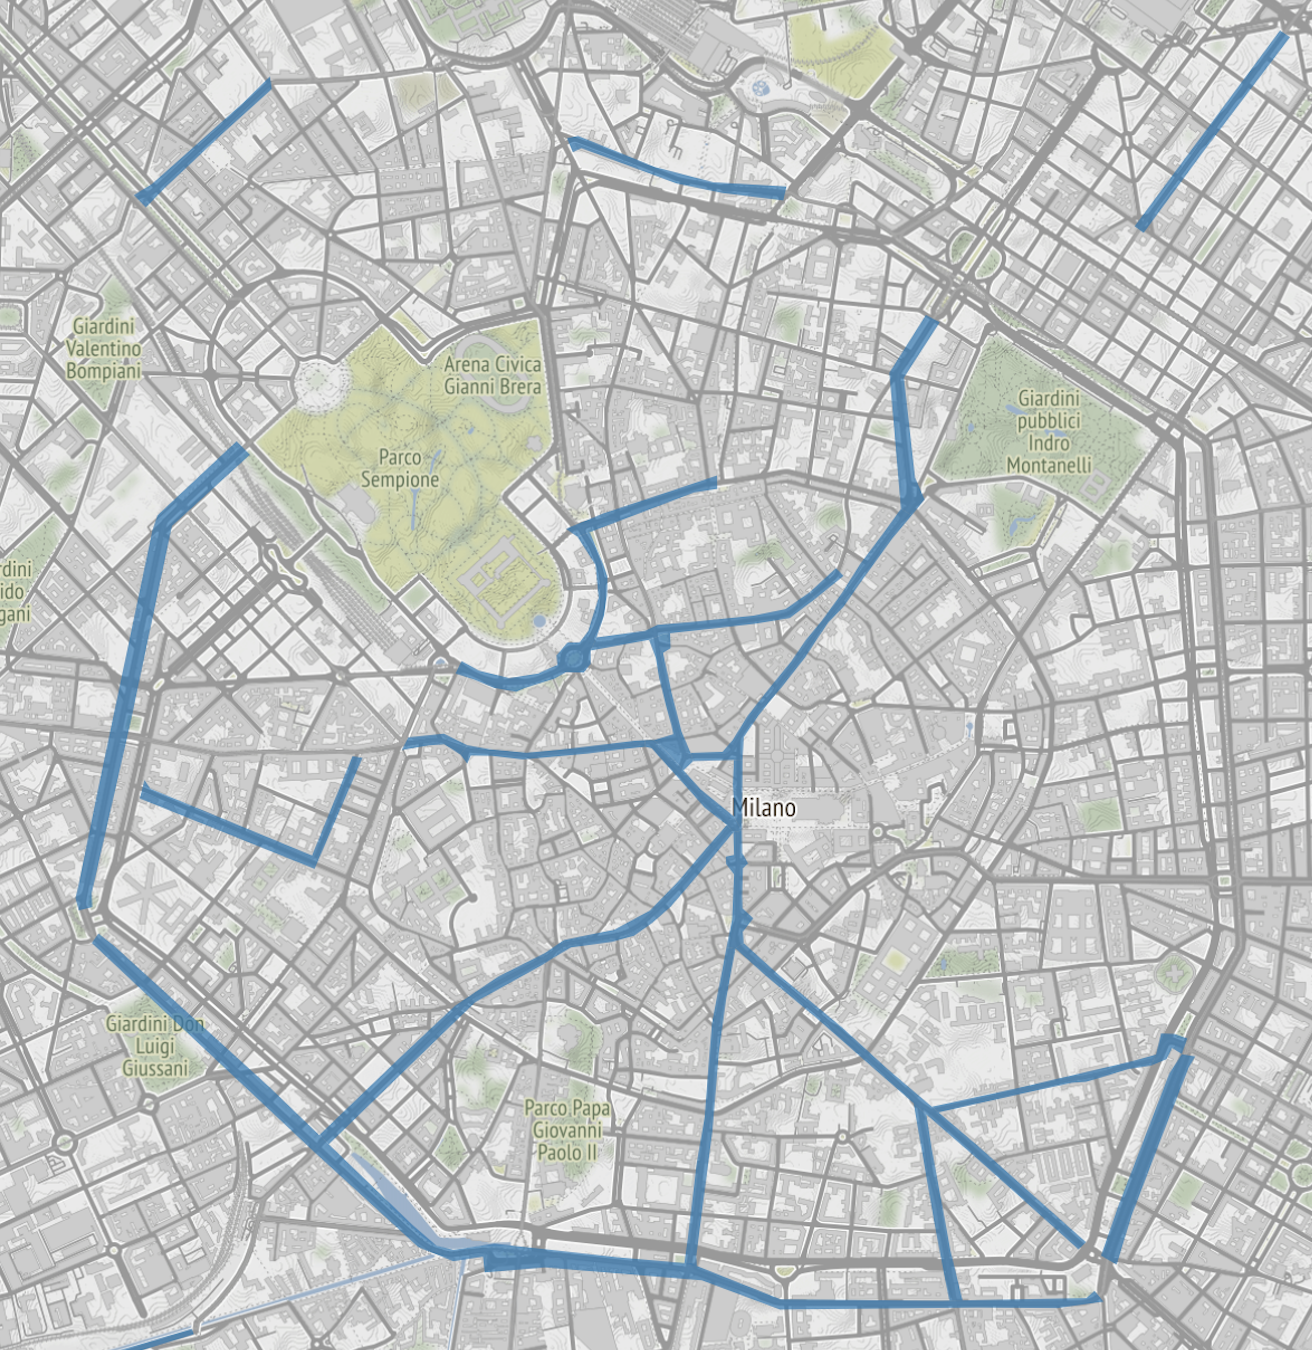
\includegraphics[width=\linewidth]{../src/pave/mappa_pave.png}
    \caption{Principali strade a Milano in pavè}
    \label{fig:mappa-pave}
\end{figure}

Creata l'area delle strade in pavè, è possibile calcolare quanti sono gli incidenti che 
avvengono in queste zone e confrontarlo con il numero di incidenti nelle strade asfaltate.

\begin{lstlisting}
    inc_in_pave = 0
    for rect in pave['geometry']: 
        rect = geometry.Polygon(rect)

        for point in incidenti['geometry']: 
            if rect.contains(geometry.Point(point)): 
                inc_in_pave += 1

    area_pave = 0
    for rect in pave['geometry']: 
        area_pave += geometry.Polygon(rect).area

    incidenti_per_km = inc_in_pave * 10**6 / area_pave
\end{lstlisting}

Il numero di incidenti per chilometro quadrato, nelle strade in pavè è  $229.45$, che è un valore 
particolarmente alto, anche se viene confrontato con il numero di incidenti nel centro storico, cioè circa 130.
Tuttavia, bisogna tenere in considerazione che il dataset che è appena stato creato, contiene solamente 
strade, senza alcuna zona morta, come edifici, a differenza dell'area utilizzata del centro storico, 
che contiene tutto il territorio del centro.

Per ovviare a questo problema, si è creato un campione di strade asfaltate, prese circa 
nella stessa zona di Milano, queste strade sono raffigurate nella mappa \ref{fig:mappa-asfalto}. 
Si è inoltre tentato di tenere i due campioni di strade il più simili possibili, sia per zona, 
sia per area totale del dataset.

\begin{figure}
    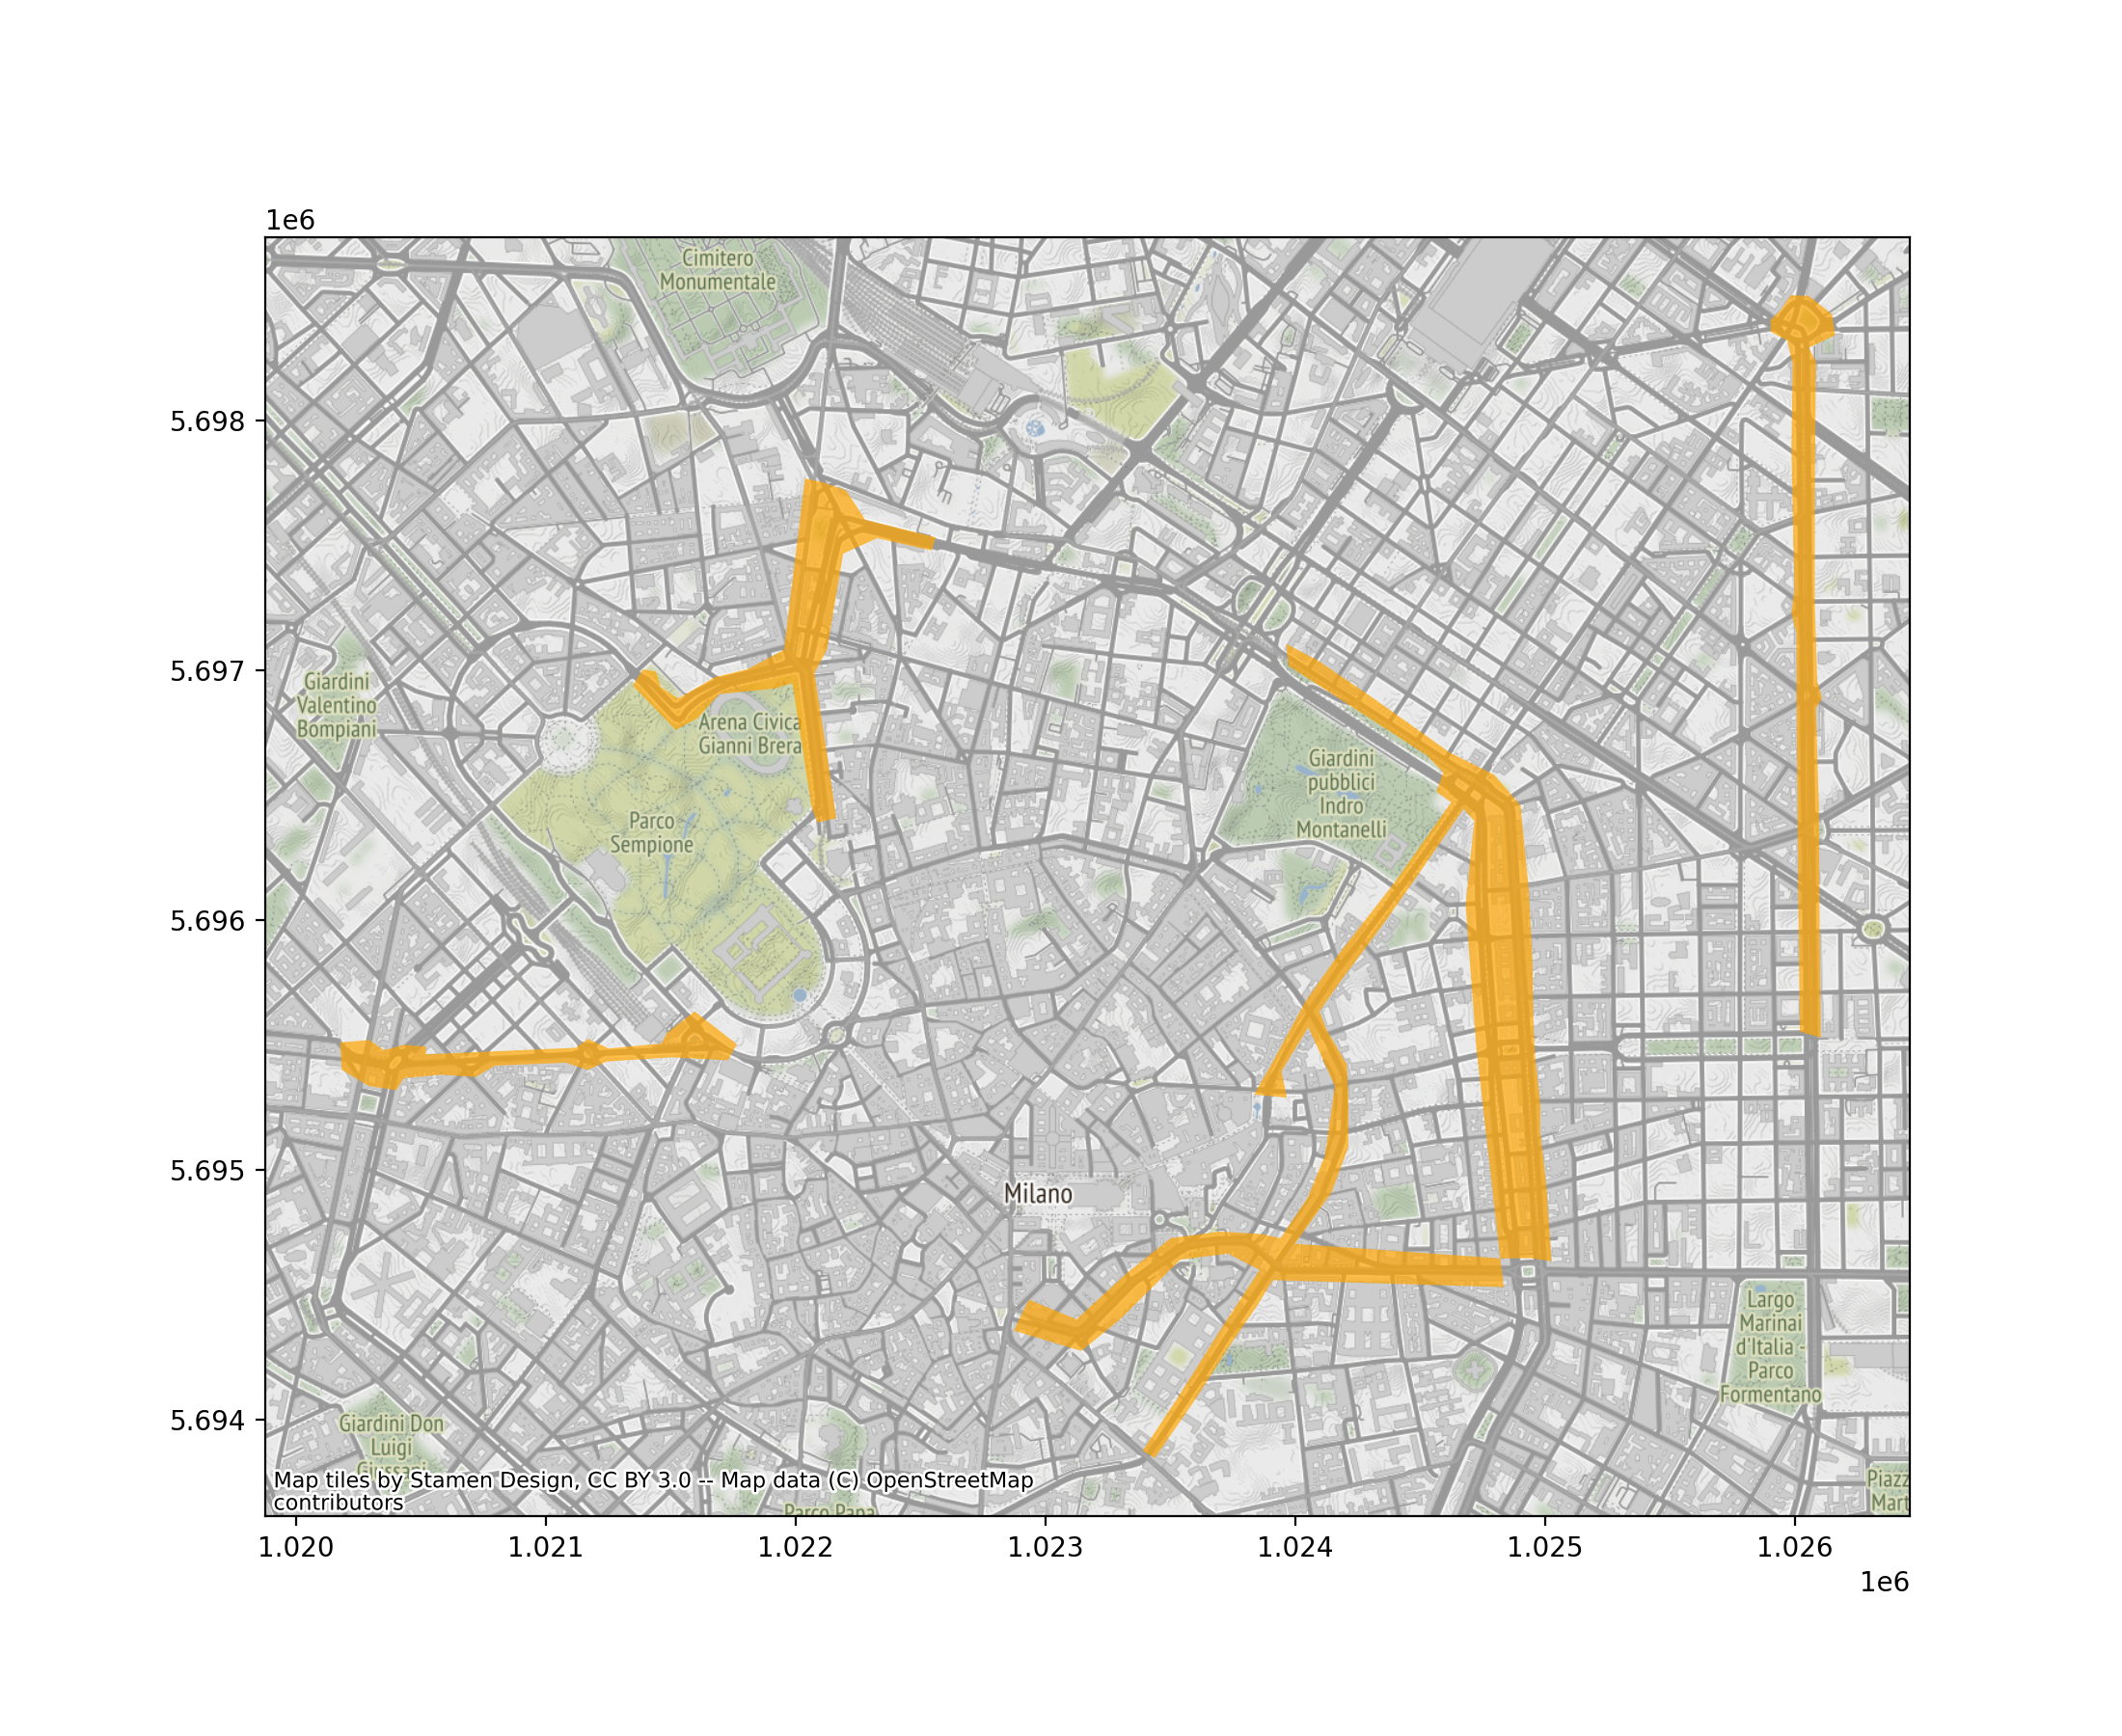
\includegraphics[width=\linewidth]{../src/pave/mappa_asfalto.png}
    \caption{Campione di strade asfaltate a Milano}
    \label{fig:mappa-asfalto}
\end{figure}

Eseguendo lo stesso calcolo realizzato per le strade in pavè, risulta che il numero di incidenti per 
chilometro quadrato, nel campione creato, è di $220.89$ incidenti.
Tuttavia, nel campione delle strade asfaltata sono stati presi vari tratti provenienti dalla circonvallazione 
interna e altre zone trafficate, mentre il campione di strade in pavè contiene, per mancanza di altri dati, 
molte strade del centro storico inevitabilmente meno trafficate.

%\clearpage
\section{Incidenti e Autovelox}

Per sapere se gli autovelox hanno influenza sull'incidentalità, 
bisognerebbe innanzi tutto sapere quando sono stati posizionati i dispositivi, e solo a quel punto, 
avendo dati su incidenti prima e dopo l'installazione, sarebbe possibile trarre conclusioni.

Alcuni dati sull'installazione di autovelox esistono per l'anno 2014, visualizzabili nella 
tabella \ref{ztl-milano}, tuttavia i dati 
riguardo agli incidenti sono solo riguardanti l'anno 2016, in quanto Istat non ha rilasciato 
le posizioni degli incidenti in altre annate.

Sapendo le posizioni degli autovelox, con un po' di lavoro manuale, è possibile ricondursi alla 
posizione effettiva sulla mappa.
Per fare ciò, la soluzione più veloce è stata quella di enumerare, 
come raffigurato nella mappa sul lato sinistro della figura \ref{fig:autovelox-indici}, 
tutti gli autovelox sulla mappa, e confrontarli con le vie della tabella.

\begin{lstlisting}[language=Python]
    path = "dataset/autovelox/autovelox_milano.geojson"
    autovelox = gp.read_file(path).to_crs(epsg=3857)
    layer_autovelox = autovelox.plot(figsize=(11,9), color="red")
    
    index = 0
    for lat, lon in geo_utils.parse_geojson_point_list(autovelox['geometry'].astype(str)):
    layer_autovelox.text(lat, lon, s=index)
    index += 1
    
    cx.add_basemap(ax=layer_autovelox)
    plt.show()
\end{lstlisting}

\begin{figure}
    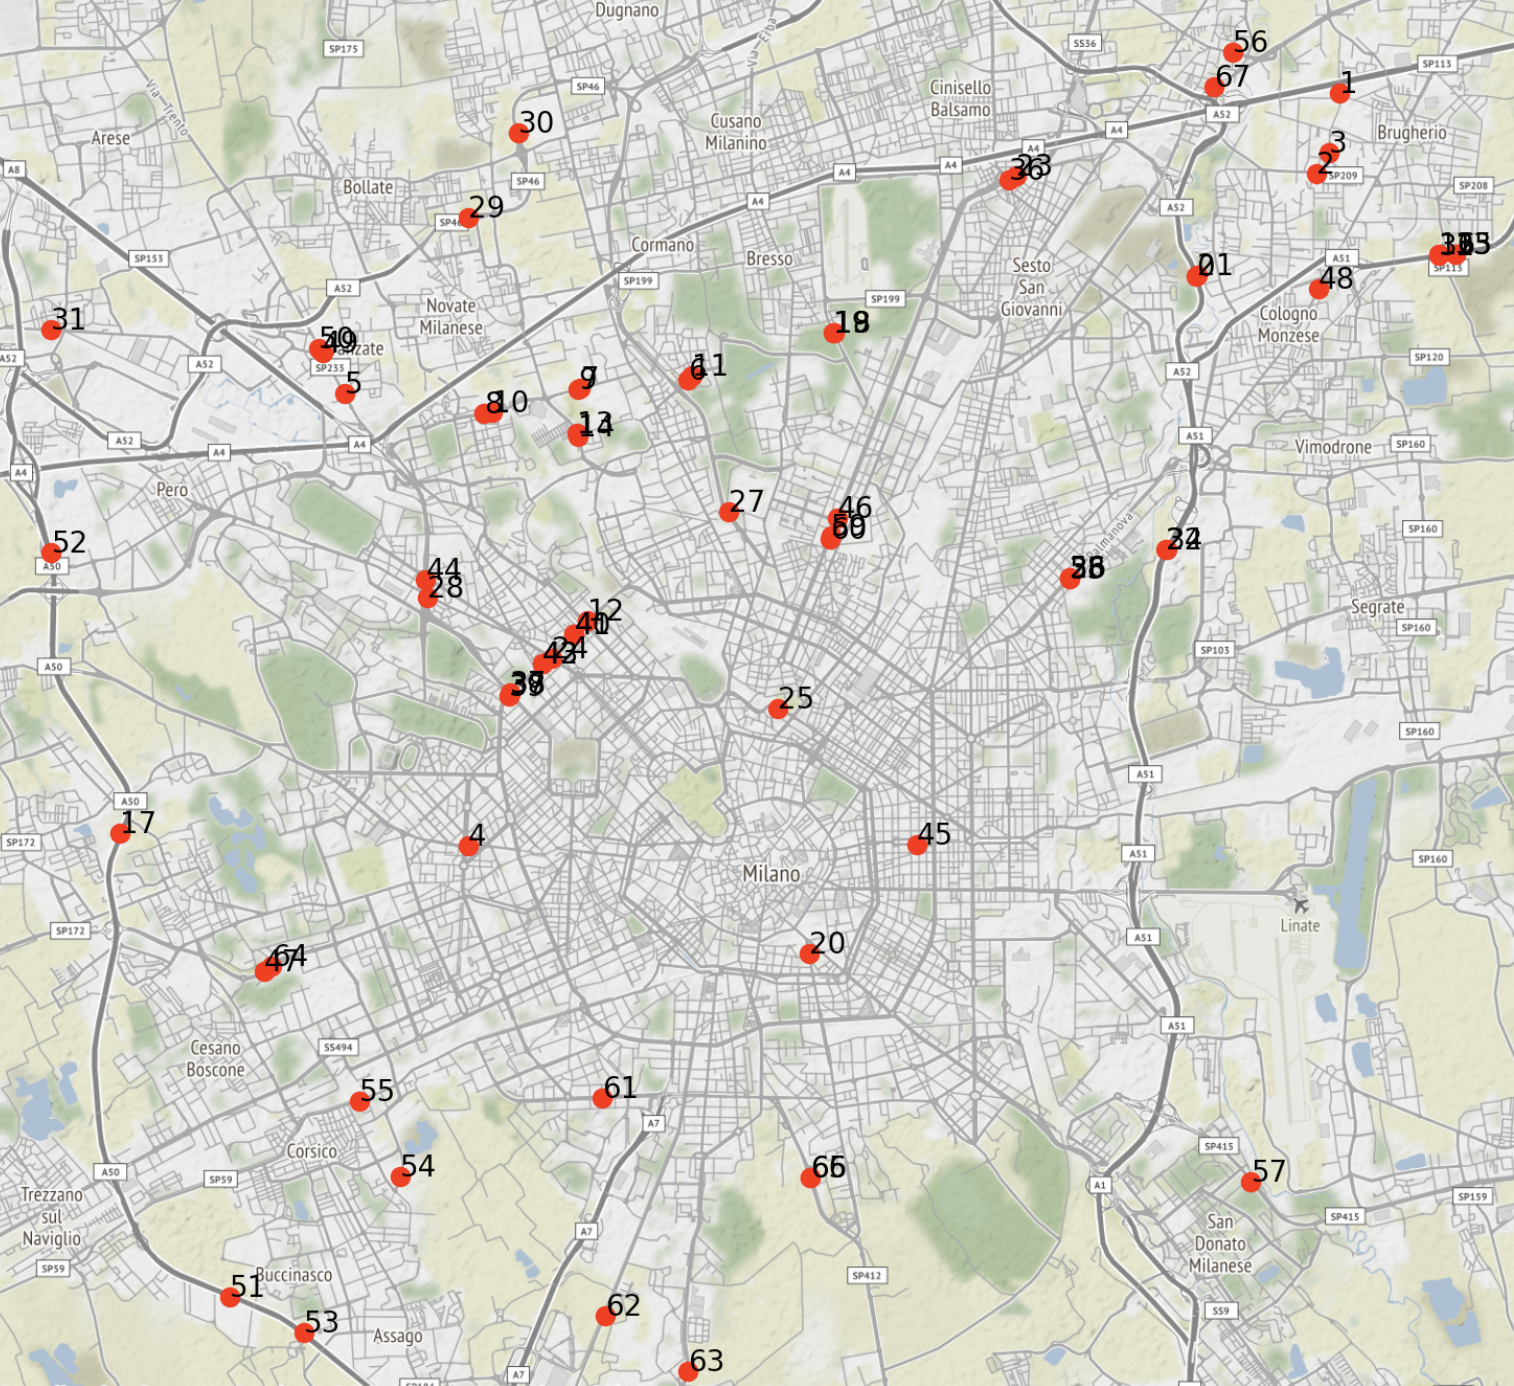
\includegraphics[width=0.6\linewidth]{../src/autovelox/autovelox_indici.png}
    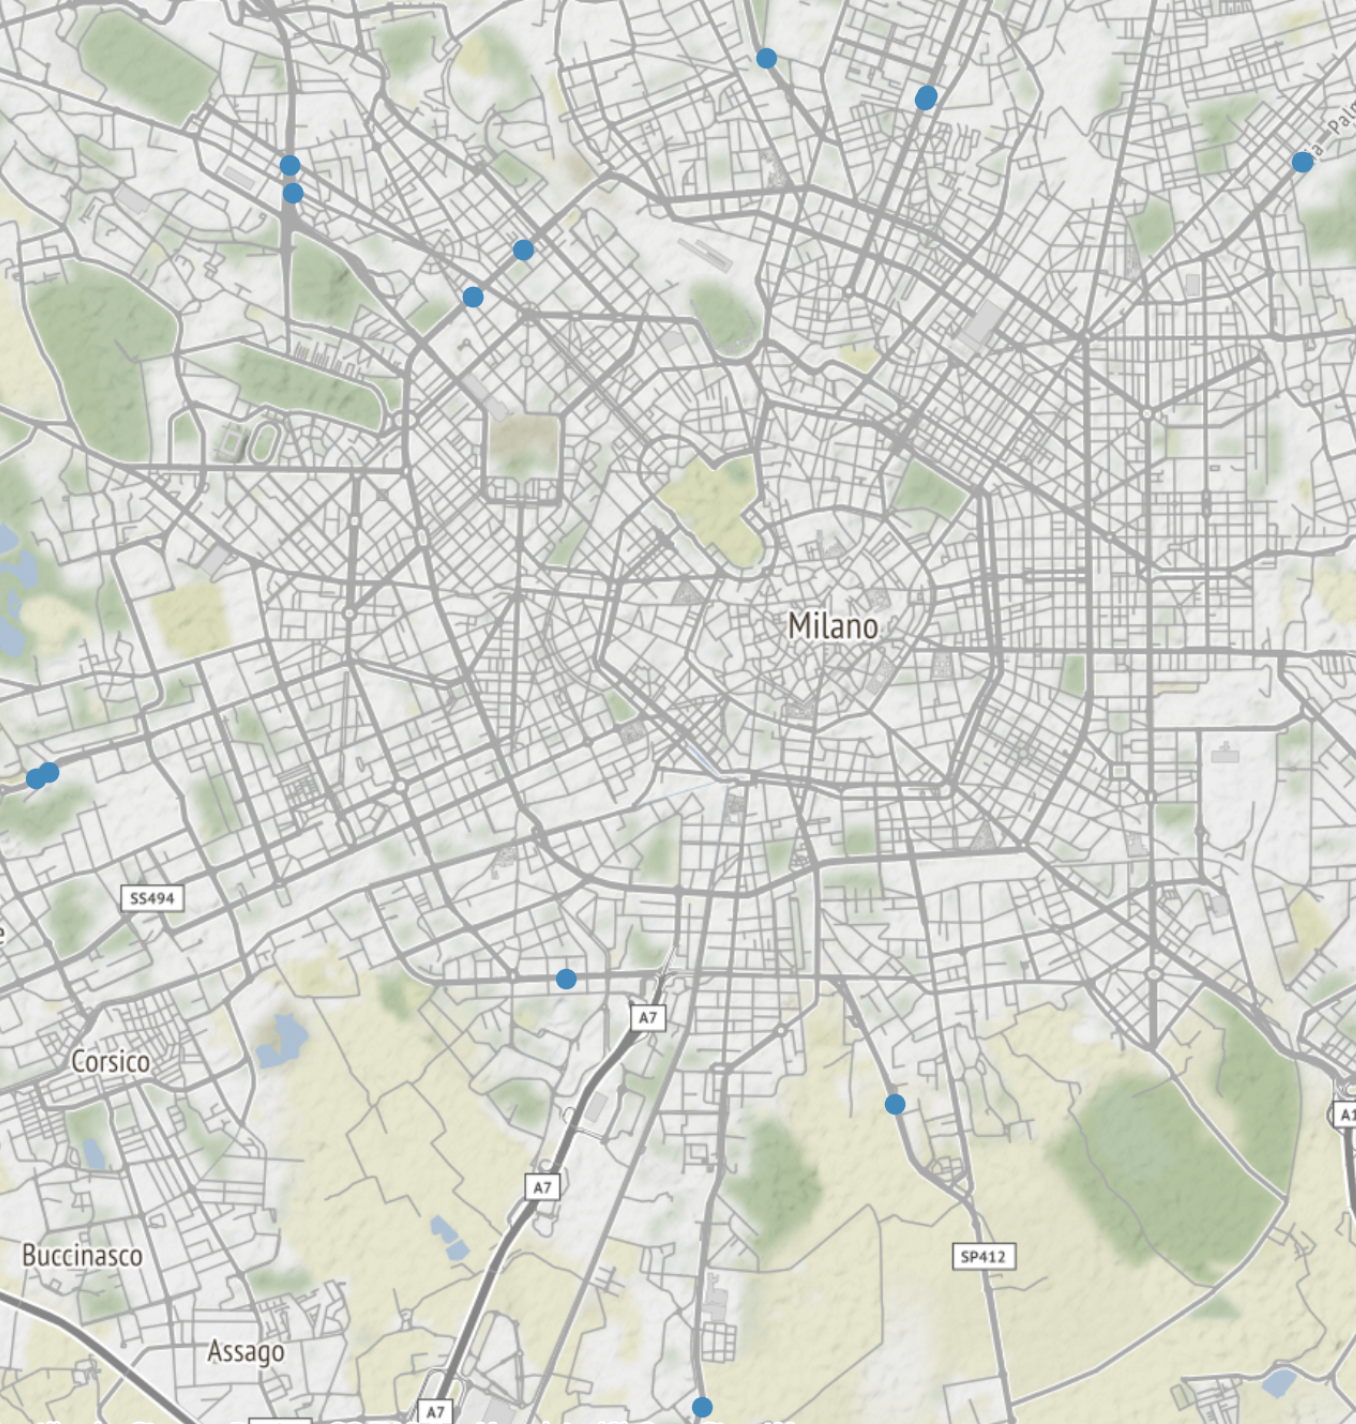
\includegraphics[width=0.4\linewidth]{../src/autovelox/autovelox_2014.png}
    \caption{Autovelox enumerati per facilitarne l'identificazione nel dataset}
    \label{fig:autovelox-indici}
\end{figure}

Una volta identificate le linee corrette del dataset, è possibile separarli dal datset completo.
Gli autovelox installati nel 2014, sono rappresentati nella mappa sul lato destro della 
figura \ref{fig:autovelox-indici}.

Per quanto non si disponga delle informazioni sugli incidenti prima e dopo dell'installazione, 
è comunque possibile sovrapporre i dataset, per vedere se gli autovelox hanno un qualche tipo di 
effetto sugli incidenti, visto che i dati sui sinistri risalgono al 2016.

\begin{figure}
    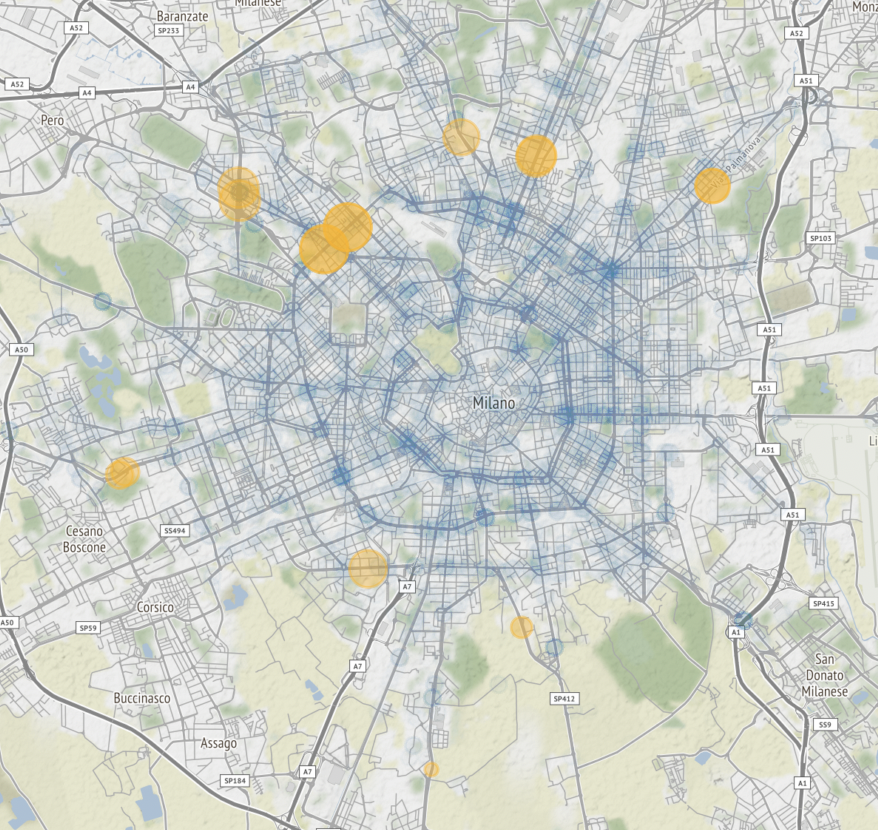
\includegraphics[width=\linewidth]{../src/autovelox/correlazione.png}
    \caption{Autovelox e Incidenti a Milano}
    \label{fig:autovelox-incidenti}
\end{figure}

La mappa \ref{fig:autovelox-incidenti} è stata realizzata contando gli incidenti avvenuti 
vicino, più precisamente nel raggio di un chilometro, a ogni autovelox.
Va precisato che le 'bolle' non indicano il raggio di conteggio degli incidenti, ma 
l'entità del numero dei sinistri trovati.

\begin{center}
    \def\arraystretch{1.5}% 
    \begin{tabular}{ |c|c|c| }
        \hline
        Autovelox & Incidenti Totali & Incidenti per $Km^2$ \\ 
        \hline
        \rowcolor{TableGray}
        0    &    194   &      61.78\\
        1    &    202   &      64.33\\
        \rowcolor{TableGray}
        2    &    208   &      66.24\\
        3    &    212   &      67.51\\
        \rowcolor{TableGray}
        4    &    166   &      52.86\\
        5    &     95   &      30.25\\
        \rowcolor{TableGray}
        6    &    100   &      31.84\\
        7    &    180   &      57.32\\
        \rowcolor{TableGray}
        8    &     23   &       7.32\\
        9    &     57   &      18.15\\
        \rowcolor{TableGray}
        10   &    291   &      92.67\\
        11   &    290   &      92.35\\
        \rowcolor{TableGray}
        12   &    296   &      94.26\\
        13   &    296   &      94.26\\
        \rowcolor{TableGray}
        14   &    149   &      47.45\\
        15   &    149   &      47.45\\
        \hline
    \end{tabular}
\end{center}

Una volta trovati gli incidenti totali, è possile calcolare gli incidenti sulla base dell'area utilizzata.
Nel seguente codice, al dataset autovelox sono aggiunte due colonne, una contenente gli incidenti totali, 
l'altra contenente gli incidenti per chilometro.

\begin{lstlisting}
    autovelox_2014['incidenti_vicini'] = gp.GeoSeries(df)
    autovelox_2014['incidenti_pesati'] = autovelox_2014['incidenti_vicini'] / 3.14
\end{lstlisting}

Questa ultima colonna, in particolare, è divisa per 3.14 perchè l'area del cerchio è data dalla formula: 

\begin{center}
    $Area\, = \pi * r^2$
\end{center}

Poichè si sta utilizzando raggio di circa un chilometro, e si vuole ottenere il numero di incidenti per chilometro 
quadrato, l'area ottentuta è 3.14.

%\clearpage
\section{Incidenti e Meteo}

%%%%%%%%%%%%%%%%%%%%%%%%%%%%%%%%%%%%%%%%%%%%%%%%%%%%%%
%\clearpage
\chapter{Dati su Incidenti}

Per quanto riguarda dati generali su incidenti in Italia, sono disponibili due dataset molto ampi, 
il primo, rilasciato da Istat, contiene dati dal 2010 al 2018 che riguardano campi come data, ora, 
numero di persone a bordo, tipo di incrocio, tipo di veicolo, ecc..
Il secondo è invece messo a disposizione da Automobile Club D'Italia (ACI) che contiene dati simili, 
ma in più mette a disposizione il luogo dell'incidente, come autostrada o strada provinciale.

%\clearpage
\section{Dati Istat su veicoli}

Il dataset Istat contiene molte informazioni riguardanti i conducenti dei veicoli coinvolti 
nell'incidente, oltre al tipo di veicoli.

%\clearpage
\subsection{Il tipo di veicolo dipende dalla strada?}


\begin{lstlisting}[language=Python]
    strade_urbane = data[(data['localizzazione_incidente'] == 1) | (data['localizzazione_incidente'] == 2) | (data['localizzazione_incidente'] == 3)]['tipo_veicolo_a']
    strade_extraurbane = data[(data['localizzazione_incidente'] == 4) | (data['localizzazione_incidente'] == 5) | (data['localizzazione_incidente'] == 6)]['tipo_veicolo_a']

    # Dove 1,2,3 sono gli ID dei diversi tipi di strade urbane, 
    # mentre 4,5,6 gli ID delle strade extraurbane
\end{lstlisting}

Il grafo \ref{fig:differenza-strade} rappresenta quali sono i veicoli coinvolti con più frequenza 
in sinistri, per tre tipi di strade diverse. Le percentuali sono calcolate per gruppo, quindi sommando 
tutte le righe di, per esempio Autostrade, si ottiene $1$.\\
Nonostante le auto private siano di gran lunga il tipo di veicolo 
più coinvolto in incidenti, nelle autostrade non sono presenti molti incidenti con motocicli, 
mentre cresce molto il numero di questi nelle strade urbane.

\begin{figure}
    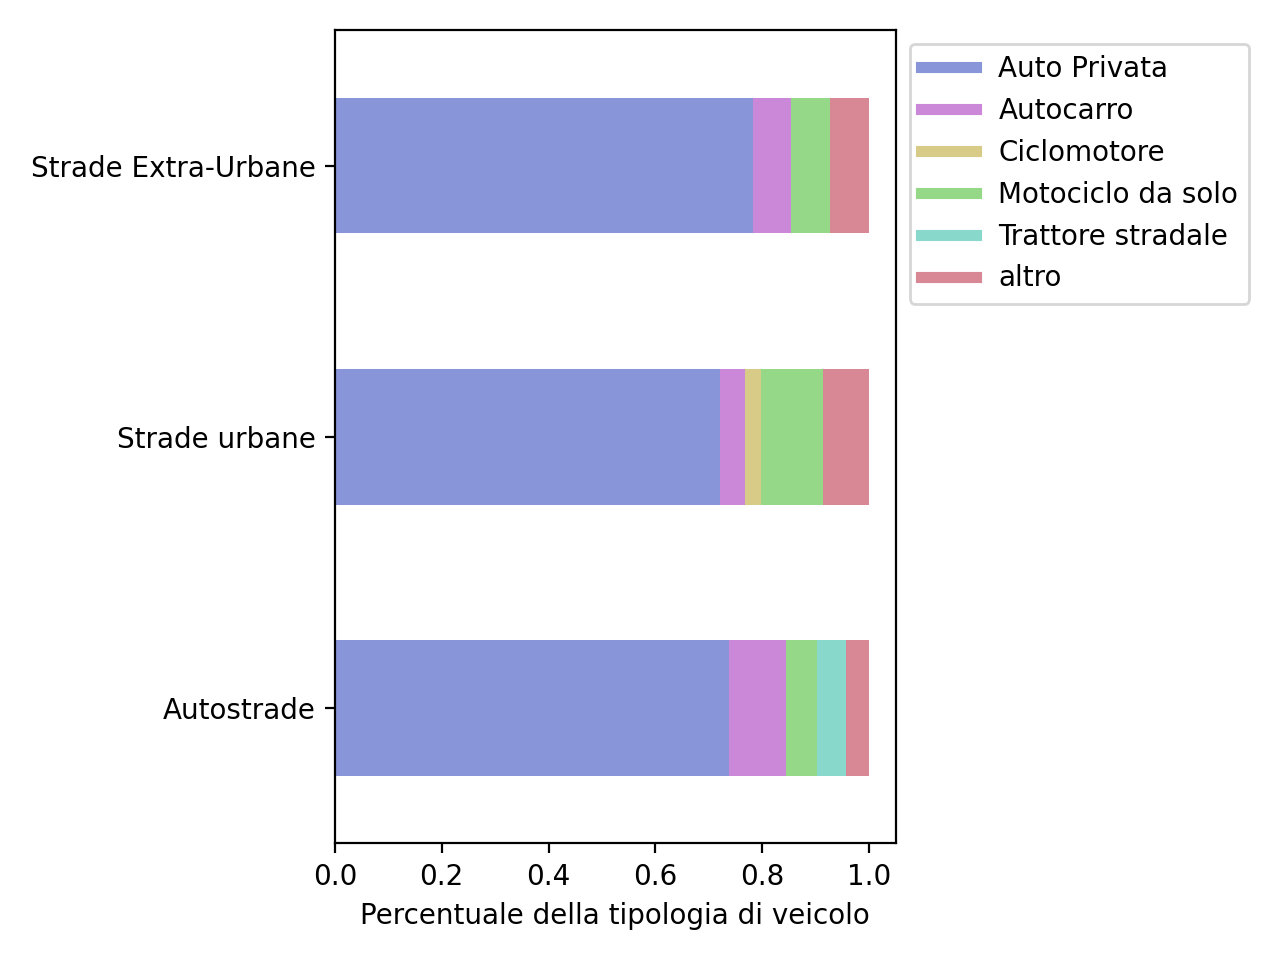
\includegraphics[width=\linewidth]{../src/incidenti/incidenti_senza_coords/tipo_veicoli/differenza_strade.png}
    \caption{Incidenti per tipo di veicolo nel 2018}
    \label{fig:differenza-strade}
\end{figure}

%\clearpage
\section{Dati Istat su conducente}

%\clearpage
\subsection{Esistono differenze tra la guida di un uomo e quella di una donna?}

\begin{figure}
    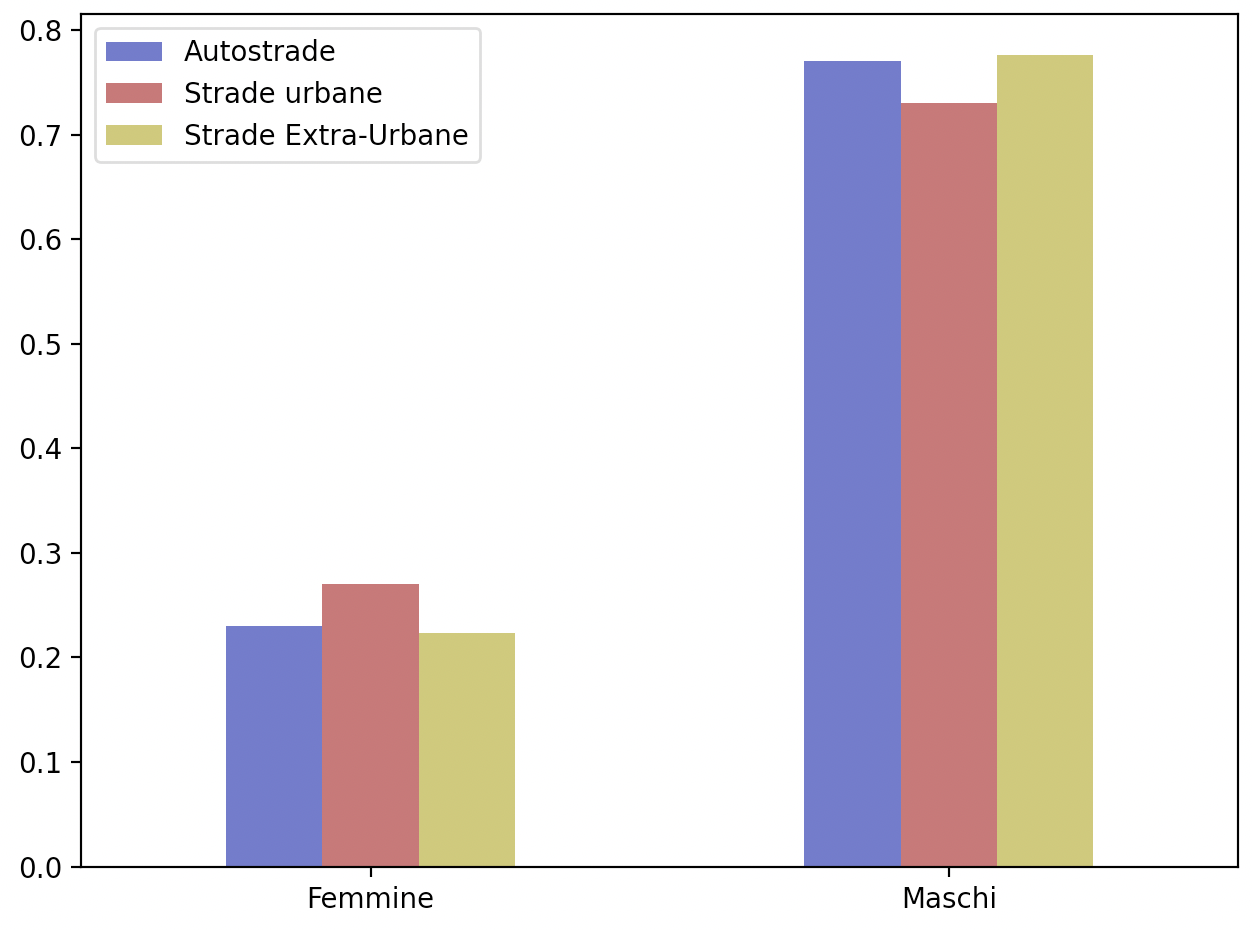
\includegraphics[width=\linewidth]{../src/incidenti/incidenti_senza_coords/tipo_veicoli/uomo-donna.png}
    \caption{Sesso del conducente per tipo di veicolo nel 2018}
    \label{fig:differenza-uomo-donna}
\end{figure}

Il grafo \ref{fig:differenza-uomo-donna} mostra che non c'è molta differenza tra i vari tipi di 
strada, per quanto riguarda il sesso del coducente.\\
Il numero di incidenti per genere è tende ad essere 75\% circa uomini e 25\% donne.
Nelle strade  urbane, la percentuale di incidenti con conducente donna aumenta leggermente nel 2010, 
questo vale per tutti gli anni?

\begin{center}
    \def\arraystretch{1.5}% 
    \begin{tabular}{ |c|c|c|c| }
        \hline
        Anno & Sesso & Autostrade & Strade Urbane \\ 
        \hline
        \rowcolor{TableGray}
        2018 & Uomo & 77\%  & 73\% \\
        2018 & Donna & 23\% & 27\% \\
        \rowcolor{TableGray}
        2016 & Uomo & 75.8\%  & 71.9\% \\
        2016 & Donna & 24.2\% & 28.1\% \\
        \rowcolor{TableGray}
        2014 & Uomo & 74.2\%  & 70.7\% \\
        2014 & Donna & 25.8\% & 29.3\% \\
        \hline
    \end{tabular}
\end{center}

In tutti gli anni la percentuale di uomini e donne coinvolti in incidenti è simile, 
questo fenomeno fa sospettare che ci siano più uomini al volante rispetto alle donne.
\'E possibile ricavare un campione per resolvere la questione. 
Dopo avere contato i conducenti delle vetture passanti a Somma Lombardo, tra le 15 e le 16 
di Giovedì, sono stati ottenuti i seguenti risultati:

\begin{center}
    \def\arraystretch{1.5}% 
    \begin{tabular}{ |c|c|c| }
        \hline
        Sesso & Numero & Percentuale \\ 
        \hline
        \rowcolor{TableGray}
        Uomini & 483 & 68.8\% \\
        Donne & 219 & 31.2\% \\
        \hline
    \end{tabular}
\end{center}

La percentuale di uomini e donne al volante è equivalente a quella degli incidenti.
Questo fatto rafforza l'idea che non ci siano differenze tra la guida di maschi e femmine.


%\clearpage
\subsection{Il numero di passeggeri influisce sull'incidentalità?}

\begin{figure}
    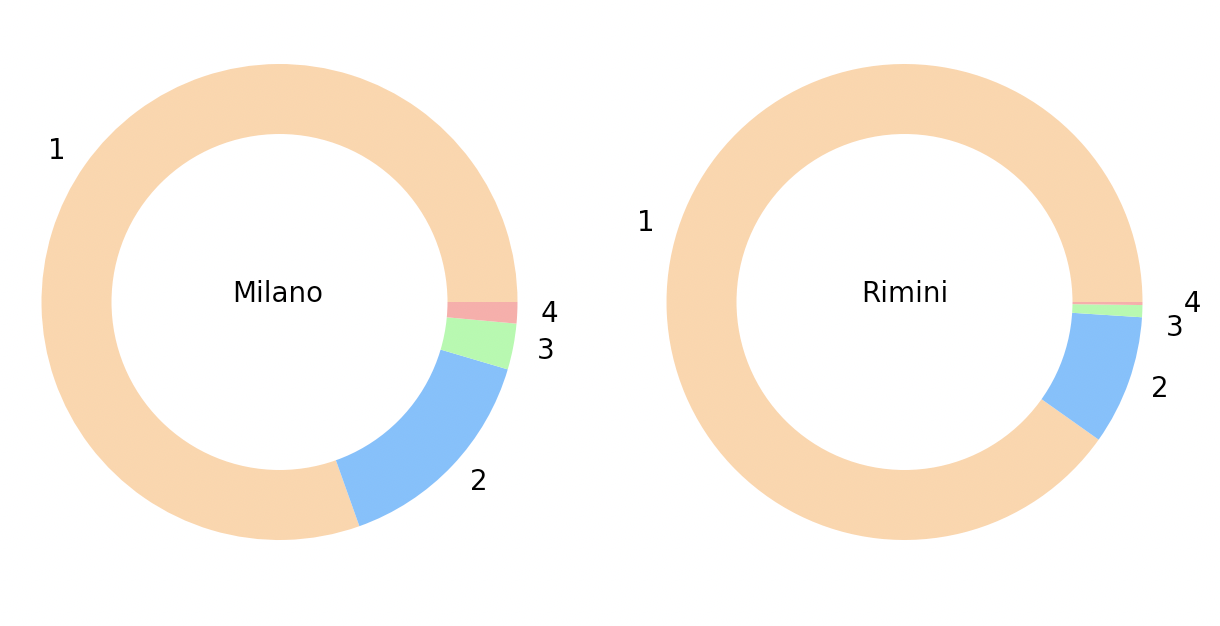
\includegraphics[width=\linewidth]{../src/incidenti/incidenti_senza_coords/tipo_veicoli/passeggeri.png}
    \caption{Numero di passeggeri in incidenti per Milano e Rimini}
    \label{fig:passeggeri-milano-rimini}
\end{figure}

La figura \ref{fig:passeggeri-milano-rimini} mostra che la maggior parte degli incidenti 
sembra avvenire quando in macchina è presente solo il conducente.
Si sono prese in considerazione le provincie di Milano e Rimini, per controllare se la località 
marittima influisse sul numero di incidenti, ma sembra che quest'ultima abbia una percentuale 
ancora più alta di incidenti in cui è presente solo il conducente, rispetto a Milano.

%\clearpage
\subsection{L'uso del telefono cellulare ha influenzato il numero di incidenti?}

Per quanto non siano disponibili dati su questo ambito, si potrebbe confrontare gli anni tra 2010 e 2013, 
in cui l'uso del cellulare in macchina ancora non era frequente, rispetto agli anni più recenti.

\begin{figure}
    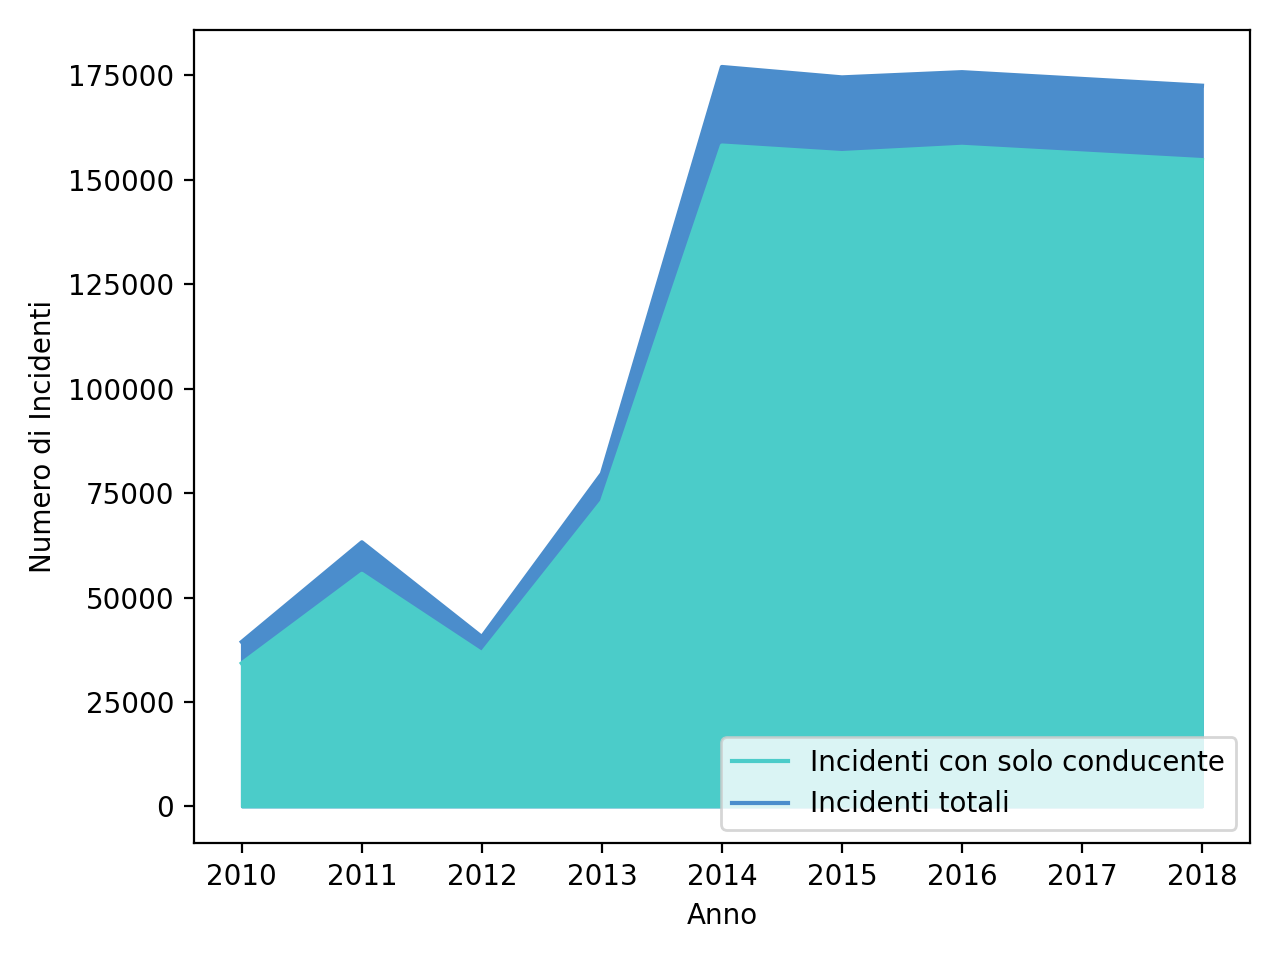
\includegraphics[width=\linewidth]{../src/incidenti/incidenti_senza_coords/anno/incremento_incidenti.png}
    \caption{Numero di incidenti all'anno, in cui è presente solo il conducente}
    \label{fig:incremento-incidenti}
\end{figure}

Nella figura \ref{fig:incremento-incidenti} è visibile come, 
tra 2013 e 2014 il numero di incidenti sia aumentato di molto, 
ma la percentuale di questi nei quali è presente solo il conducente è aumentata con essa.
Per assurdo, il numero di incidenti con più di una persona nel veicolo è aumentato maggiormente, 
ed è visibile nella separazione tra la linea blu e la linea azzurra.\\

Curiosamente, nel grafo è presente un'ampia curva, a indicare un'aumento di incidenti 
a partire dal 2014. Tuttavia dopo il 2015 il numero di incidenti tende a diminuire, il che 
fa sospettare una modifica nella metodologia di raccolta dei dati, più che un cambiamento 
nel comportamento di molte persone.\\
A supportare questa ipotesi è anche la taglia del campione totale, che aumenta molto, mentre la 
percentuale di incidenti in cui è presente solo il conducente rimane molto simile.

%\clearpage
\section{Dati Istat su orari e mesi}

%\clearpage
\subsection{Incremento dell'incidentalità in diversi orari}

Per prima cosa, con un semplice conto degli incidenti durante il weekend 
e confrontandolo con il numero di quelli avvenuti durante la 
settimana lavorativa, si osserva che nel weekend avvengono più incidenti 
durante la sera e la notte, mentre durante la settimana in giornata.

\begin{figure}
    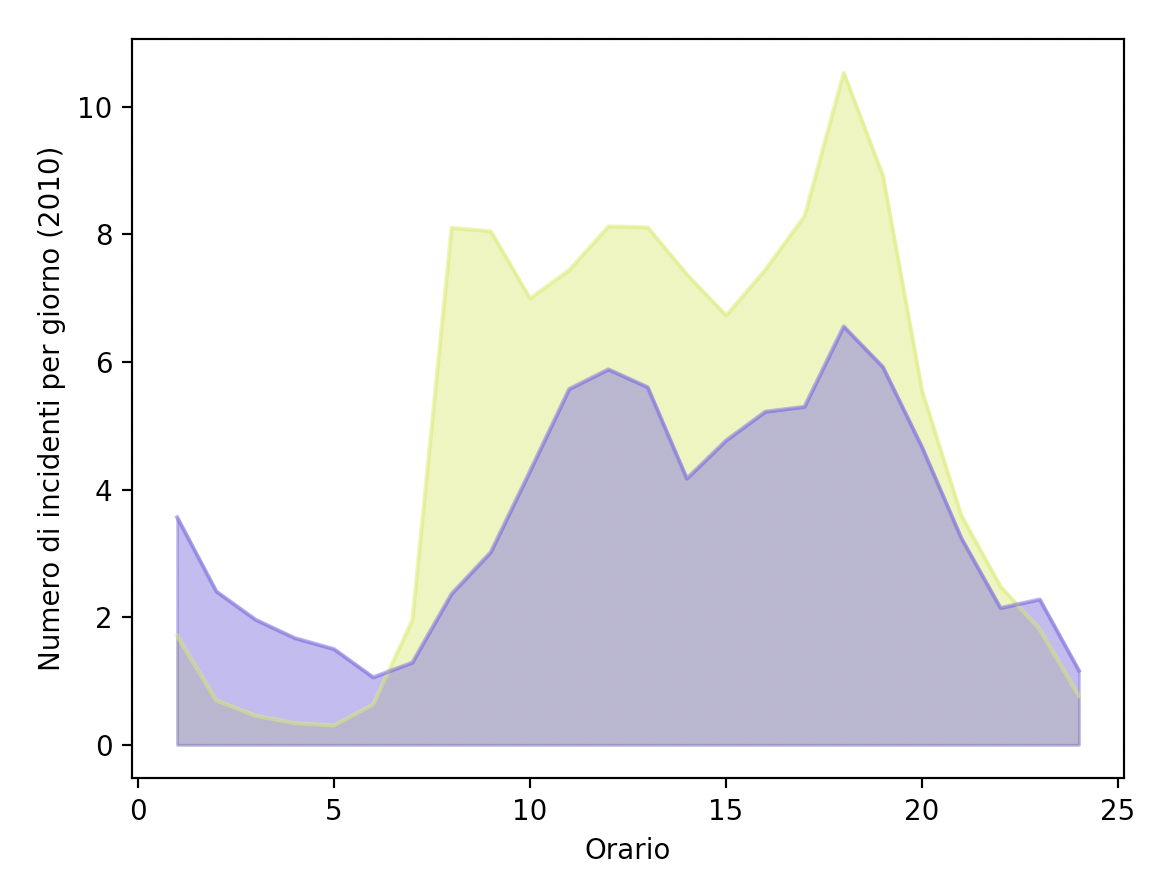
\includegraphics[width=\linewidth]{../src/incidenti/incidenti_senza_coords/ore_punta/week_weekend.png}
    \caption{Incidenti per ora}
    \label{fig:week-weekend}
\end{figure}

Per quanto riguarda gli orari di punta, sono state prese in considerazione due fasce orarie, la prima, 
mattutina dalle 7:00 alle 10:00, e la seconda pomeridiana, dalle 17:00 alle 19:00.
L'incremento durante la fascia oraria pomeridiana è subito osservabile nella figura 
\ref{fig:week-weekend}; più precisamente si 
ha un incremento del 95.2\% di incidenti rispetto alla media durante la settimana lavorativa. 
Durante il weekend invece, si osserva comunque un'incremento, ma solamente del 61.1\%.

Va sottolineato che i grafi indicano gli incidenti normalizzati per numero di 
giorni, quindi gli incidenti totali della settimana sono divisi per cinque giorni, 
mentre quelli del weekend per due.

\begin{lstlisting}[language=Python]
    ora_weekend = data[data['giorno'] > 5]['Ora'].value_counts().sort_index()
    ora_week = data[data['giorno'] < 6]['Ora'].value_counts().sort_index()

    ora_week /= 5 * 52
    ora_weekend /= 2 * 52
\end{lstlisting}

Si pu\'o osservare che nella fascia oraria delle 18:00, 
avvengono molti più sinistri, mentre nella fascia mattutina, 
il numero non sembra variare molto dalla media di incidenti durante il giorno.

%\clearpage
\subsection{Incremento dell'incidentalità nelle fasce orarie della mattina}

Se si selezionano solo gli incidenti nella provincia di Milano, mostrati nel grafo 
\ref{fig:week-weekend-milano}, è possibile individuare 
il secondo picco di incidenti, quello durante le ore di punta mattutine.
In particolare si ha un incremento del 34.3\% alle 8:00 rispetto alla media, nelle giornate lavorative;
d'altro canto, durante il weekend, il numero di incidenti cala del 58.5\% rispetto alla media.

\begin{figure}
    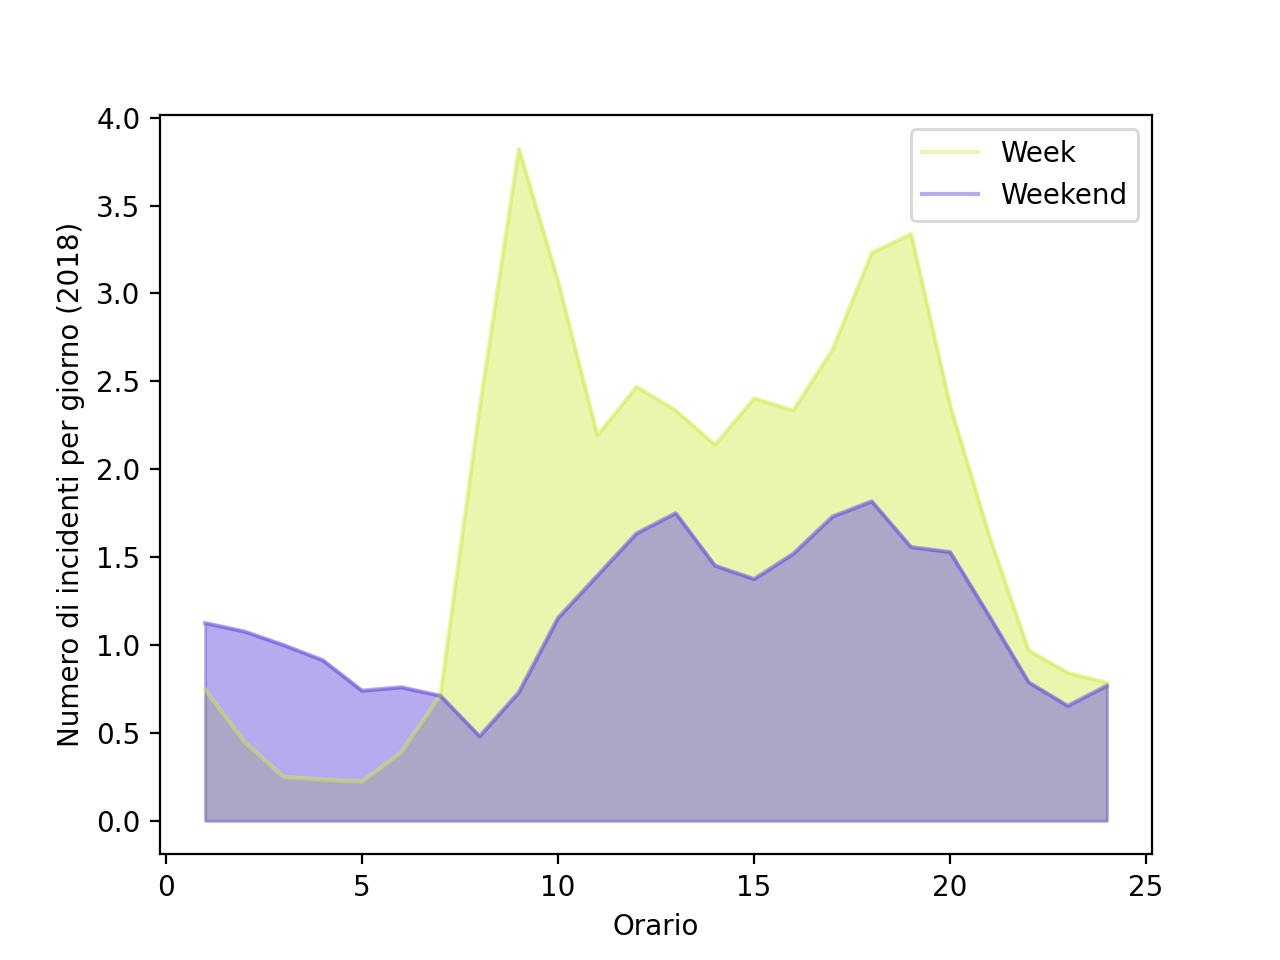
\includegraphics[width=\linewidth]{../src/incidenti/incidenti_senza_coords/ore_punta/week_weekend_milano.png}
    \caption{Incidenti per ora a Milano}
    \label{fig:week-weekend-milano}
\end{figure}

\subsection{Correlazione tra incidenti e traffico}

Sarebbe interessante calcolare quanto il traffico possa influenzare il numero di incidenti 
nelle diverse ore della giornata. \\
Un primo problema da affrontare è quello di individuare informazioni sul traffico. 
Per quanto un dataset contenente questi dati non sia stato trovato, 
è possibile realizzare una stima del traffico a Milano, 
in quanto a partire dal 2011, è disponibile il numero degli accessi all'area C.

\begin{figure}
    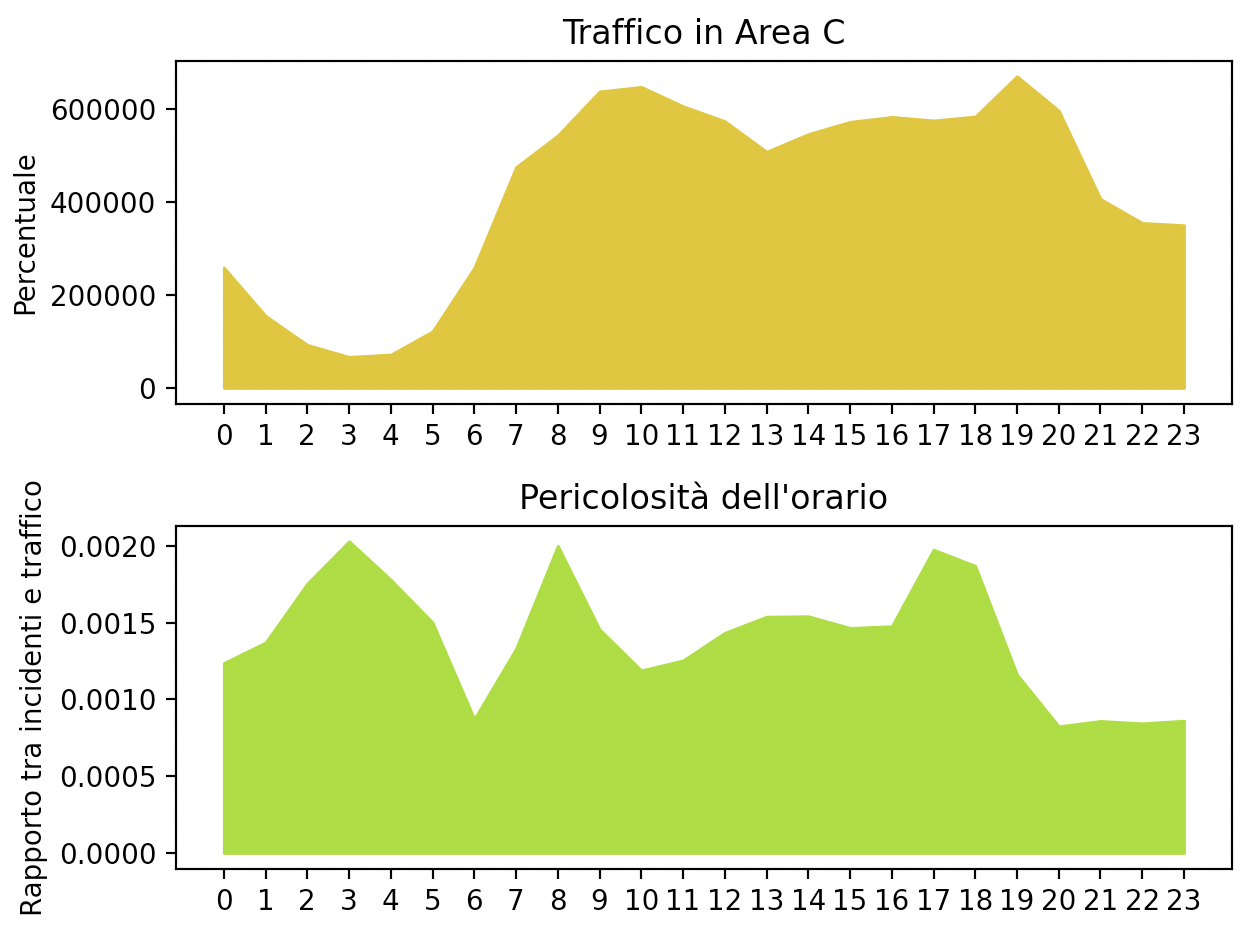
\includegraphics[width=\linewidth]{../src/area_c/rapporto_incidenti_traffico.png}
    \caption{Rapporto tra incidenti e traffico per orario a Milano}
    \label{fig:rapporto-incidenti-traffico}
\end{figure}

L'immagine \ref{fig:rapporto-incidenti-traffico} contiene, a partire dall'alto, 
la percentuale traffico in area C a una determinata ora, il numero di incidenti a Milano, 
e infine il numero di incidenti a Milano, pesati in base al traffico.\\
Gli ultimi due grafi sono estremamente simili, ciò è dovuto al fatto che il volume di traffico e 
il volume di incidenti siano fattori altamente correlati, il che comporta che non ci siano molte 
situazioni in cui il numero di incidenti sia alto in orari con poco traffico.\\

\begin{lstlisting}
    # eseguito con dati del 2016
    accessi_area_c_per_ora = pd.Series()
    for f in data['hour'].unique():
        accessi_area_c_per_ora = accessi_area_c_per_ora.append(
            pd.Series(data[data['hour'] == f]['totale'].sum()), 
            ignore_index=True
            )

    incidenti_per_ora = data[data['provincia'] == 15]['ora'].value_counts().sort_index()

    correlazione = accessi_area_c_per_ora.corr(incidenti_per_ora)
\end{lstlisting}

Correlazione tra traffico in area C a Milano e incidenti per orario è $0.877$

%\clearpage
\subsection{Incidentalità in orari notturni}

Come individuato nel grafo \ref{fig:week-weekend}, durante le 
ore notturne si ha il comportamento di incidenti tra settimana lavorativa e weekend opposta.
Nella figura \ref{fig:ore-notte}, sono raffigurate le principali ore della notte, divise tra 
settimana lavorativa e weekend.
Chiaramente, durante il weekend si hanno un maggior numero di incidenti 
negli orari serali e notturni.
Il traffico, stimato tramite gli accessi all'area C, conferma la tendenza?

\begin{figure}
    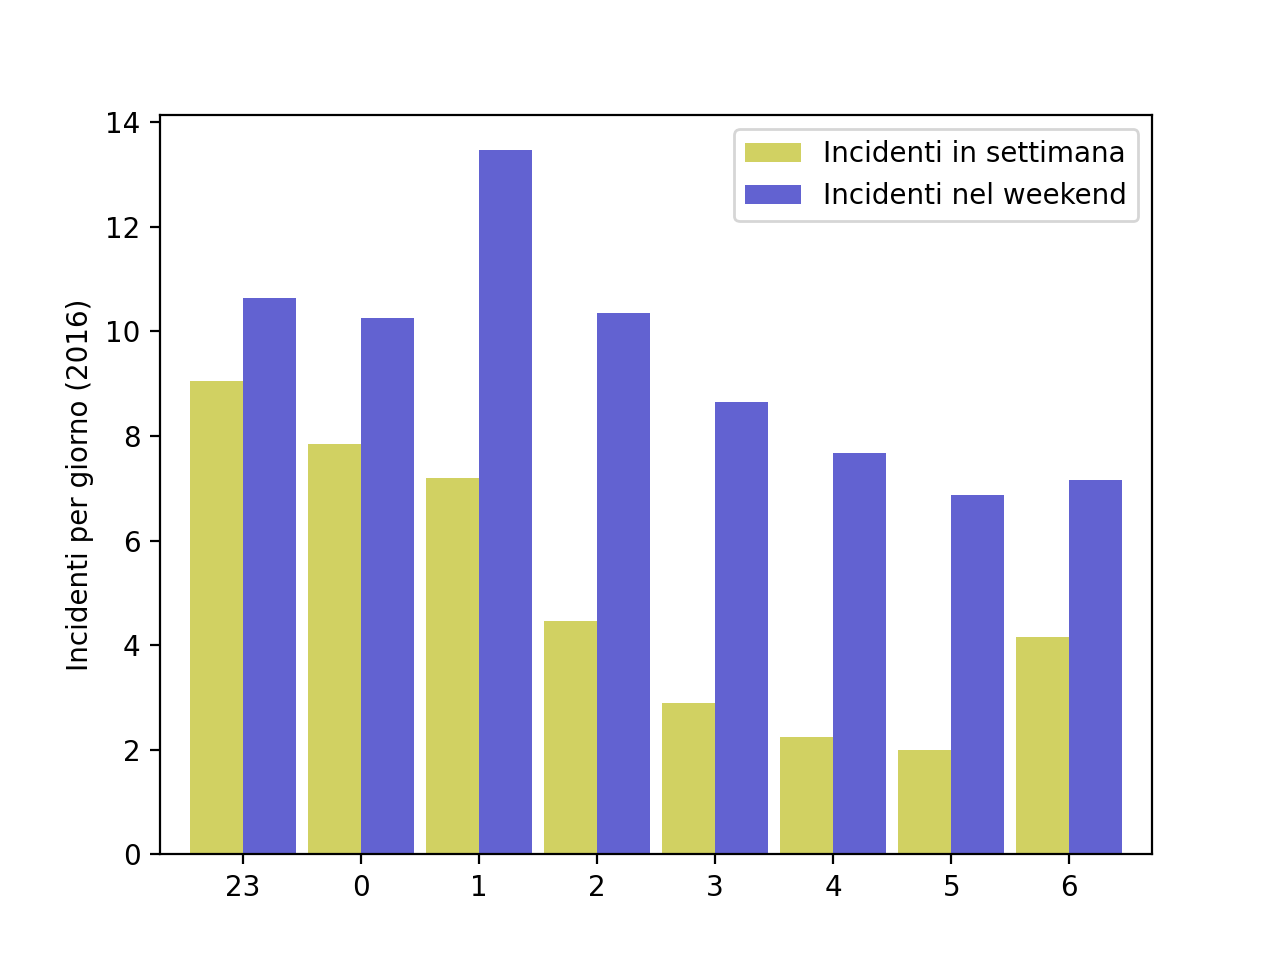
\includegraphics[width=0.5\linewidth]{../src/incidenti/incidenti_senza_coords/ore_punta/ore_notte.png}
    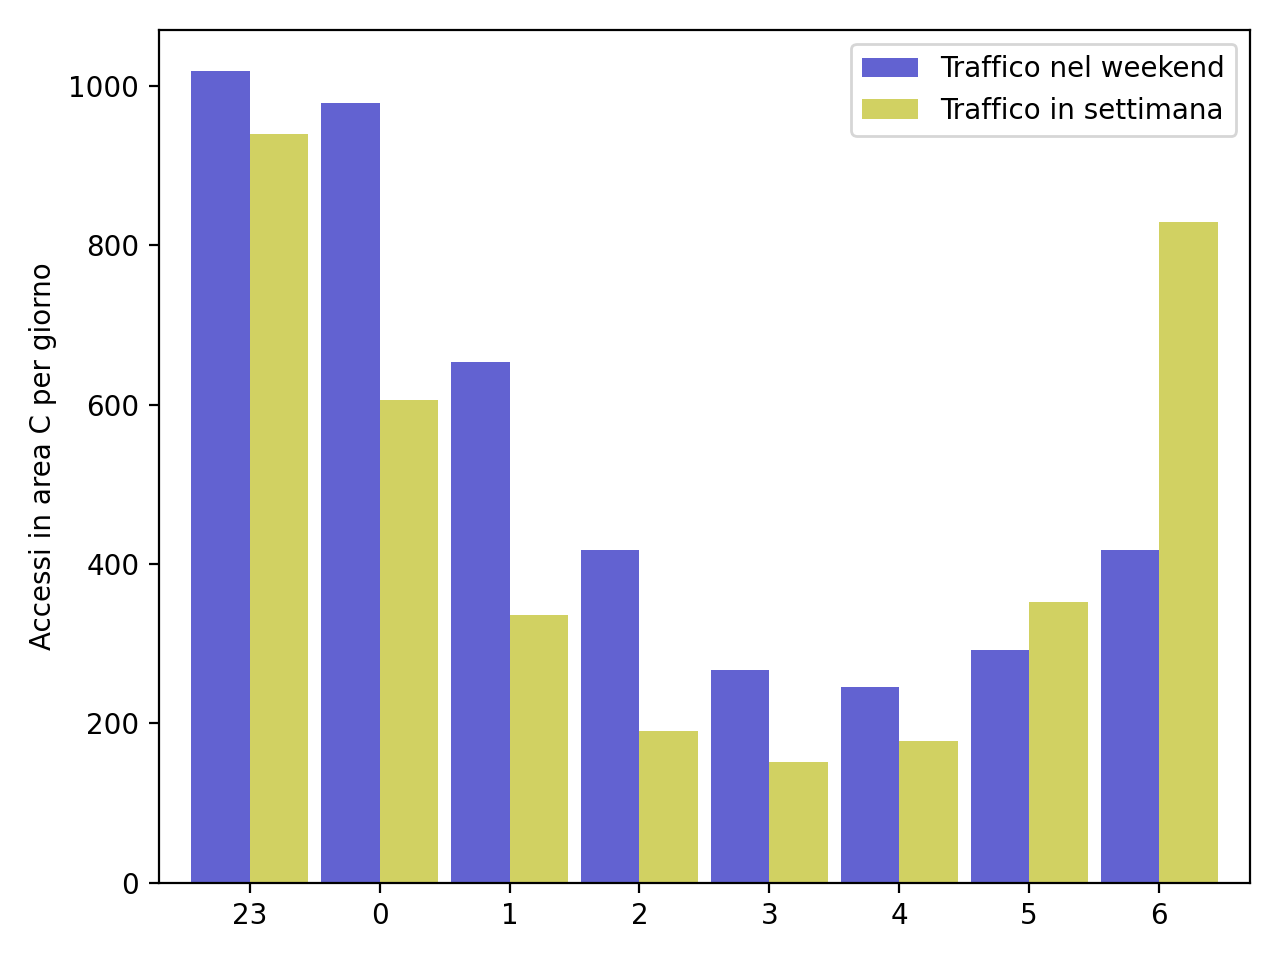
\includegraphics[width=0.5\linewidth]{../src/area_c/traffico_serale.png}
    \caption{Incidenti e traffico durante ore serali o notturne}
    \label{fig:ore-notte}
\end{figure}

Va detto che la differenza di traffico tra settimana lavorativa e weekend in orari serali non è molta, 
e che il divario maggiore è presente alle ore 6 in favore del traffico in settimana.
D'altra parte il traffico nel weekend è maggiore in quasi tutte le altre ore.

Alla luce di ciò, quali sono le ore più pericolose?
Eseguendo il rapporto tra incidenti e traffico per orario, si ottiene la figura 
\ref{fig:rapp-inc-traff}.

\begin{figure}
    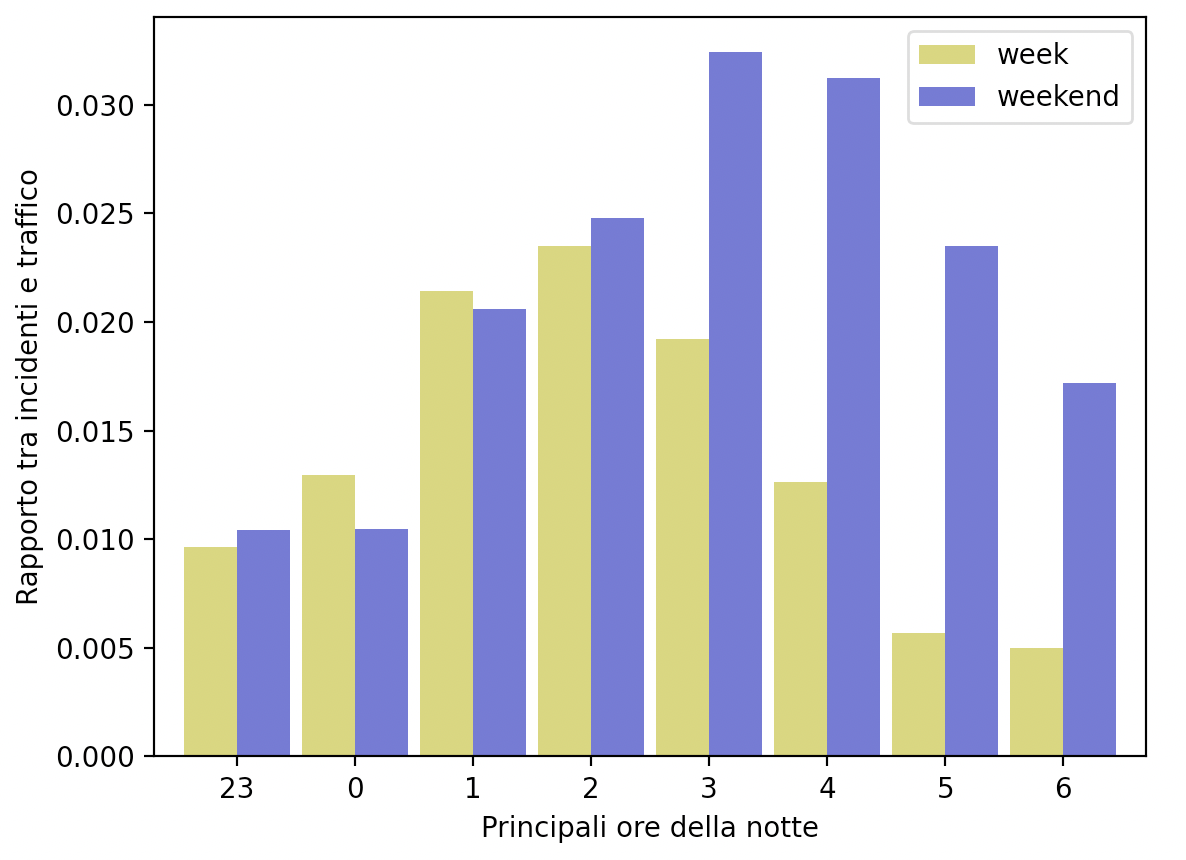
\includegraphics[width=\linewidth]{../src/area_c/rapporto_inc_traff.png}
    \caption{Rapporto tra incidenti e traffico durante ore serali o notturne}
    \label{fig:rapp-inc-traff}
\end{figure}

Per quanto riguarda il weekend, le ore più pericolose sono tra le 3:00 e le 4:00 di notte, mentre per 
la settimana lavorativa le ore più pericolose sono quelle tra 1:00 e 3:00, e il numero di 
incidenti rapportato al traffico è anche molto minore. 

%\clearpage
\subsection{Quanto influiscono le vacanze estive sull'incidentalità?}

\begin{figure}
    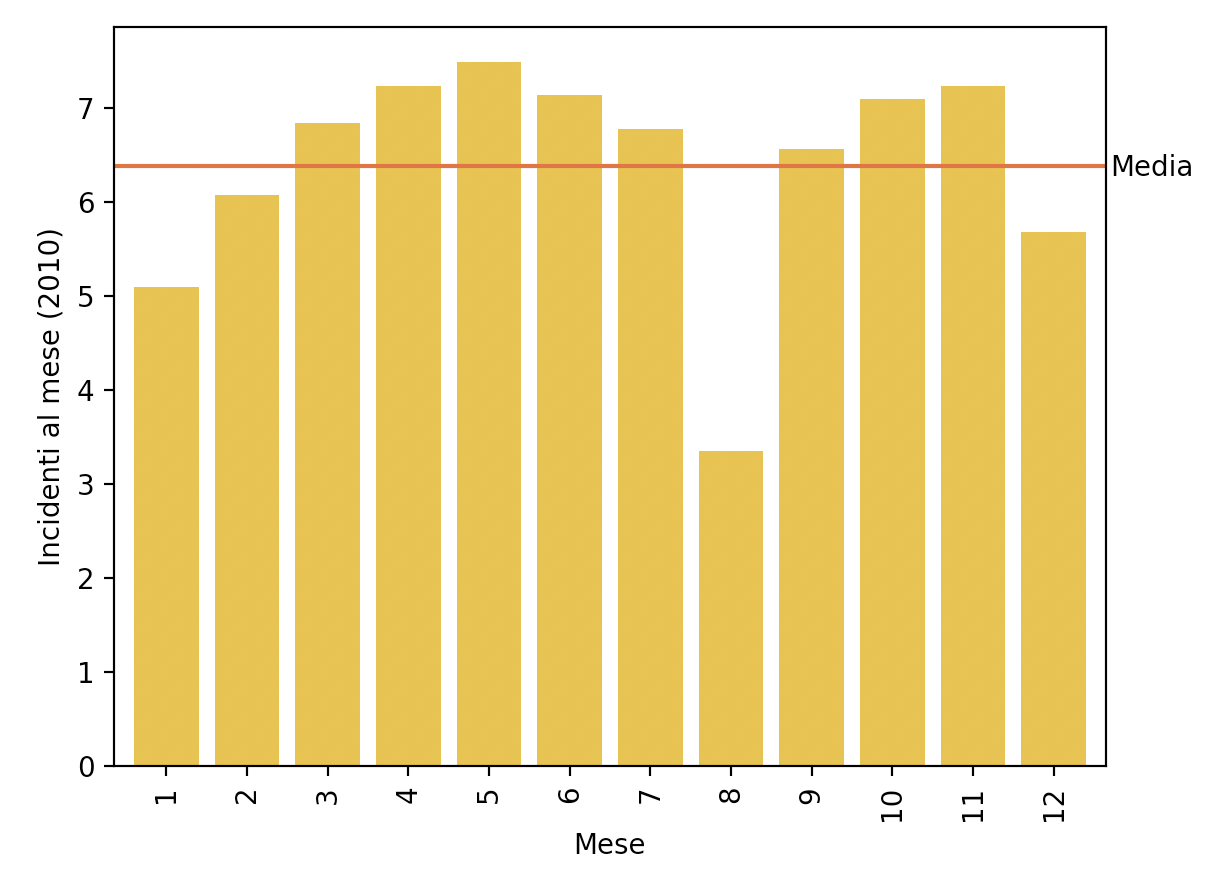
\includegraphics[width=\linewidth]{../src/incidenti/incidenti_senza_coords/mese_incidenti/milano_mese.png}
    \caption{Incidenti per mese in Milano}
    \label{fig:milano-mese}
\end{figure}

Nel grafo \ref{fig:milano-mese} si nota un chiaro calo di incidenti 
nel mese di Agosto in provincia di Milano.
\'E possibile controllare il decremento del numero di incidenti, anche per gli altri anni, 
in cui sono disponibili dati.

\begin{center}
    \def\arraystretch{1.5}%  
    \begin{tabular}{ |c|c| } 
    \hline
    Anno & Decremento in Agosto \\ 
    \hline
    2010 & 47.4\%  \\ 
    \rowcolor{TableGray}
    2011 & 35.14\% \\
    2012 & 45.46\% \\
    \rowcolor{TableGray}
    2013 & 41.37 \% \\
    \hline
    \end{tabular}
\end{center}

Per quanto riguarda gli anni successivi, il dataset non dispone più di un campo che indichi il mese 
dell'incidente, ma è disponibile soltanto il trimestre.
La figura \ref{fig:milano-trimestri} mostra la quantità di incidenti per trimestre per ogni 
anno a partire dal 2010 fino al 2018.

\begin{figure}
    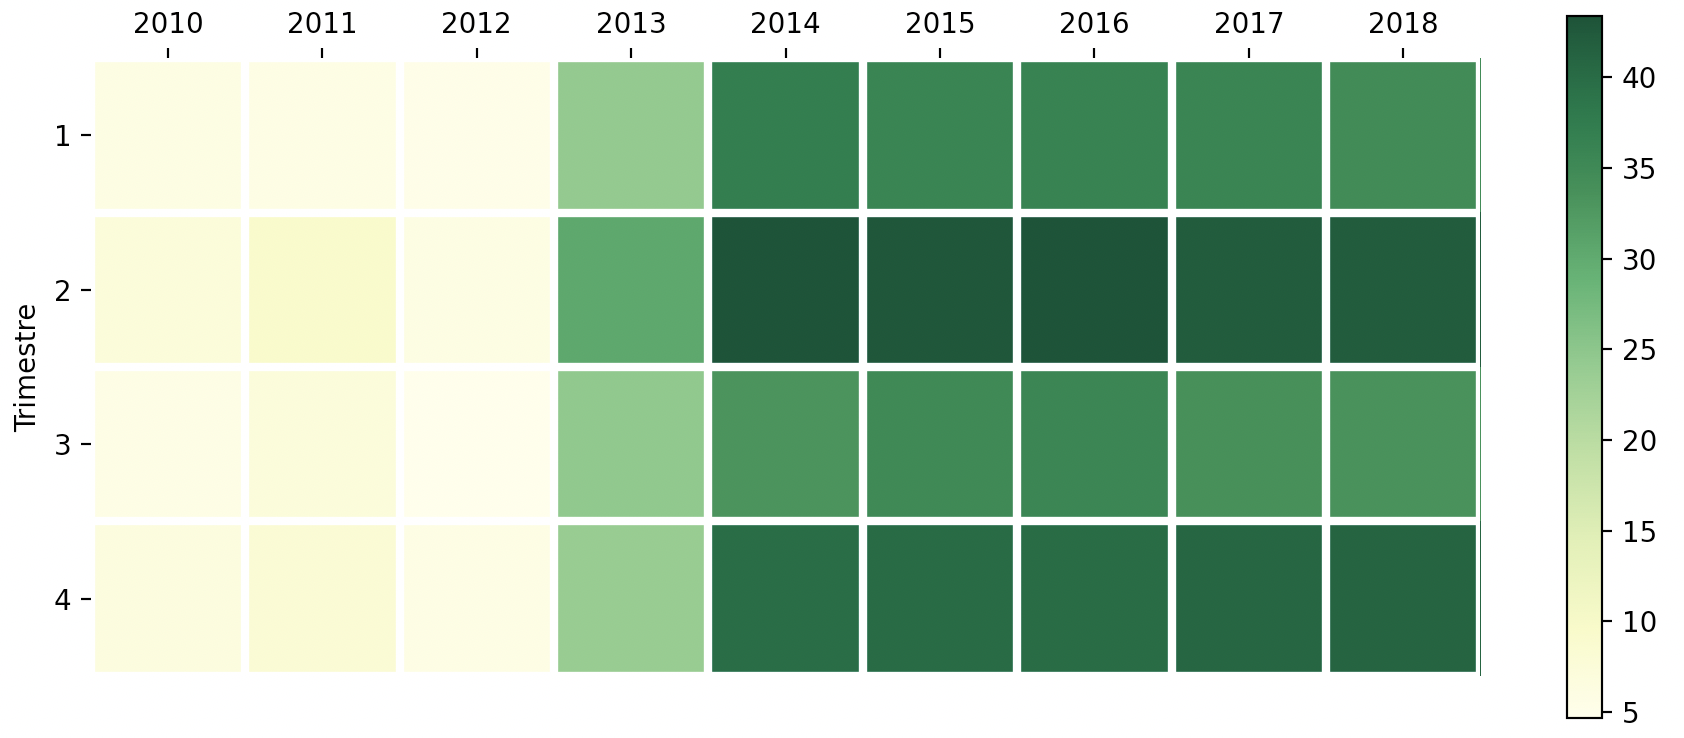
\includegraphics[width=\linewidth]{../src/incidenti/incidenti_senza_coords/mese_incidenti/trimestri.png}
    \caption{Incidenti a Milano per trimestre}
    \label{fig:milano-trimestri}
\end{figure}

Anche nel caso dei trimestri, quello estivo ha decisamente un numero minore di incidenti, 
nonostante il numero sia probabilmente alzato per la presenza di Giugno e Luglio.

Per quanto possano esserci molti fattori che contribuiscono a questa tendenza di decremento di sinistri, 
quello che influisce di più devono essere le partenze per le vacanze estive.

Un modo per testare questa teoria è controllare se il traffico durante il mese di Agosto cala a Milano, 
tuttavia, non è stato trovato alcun dataset riguardante il volume di automobili nelle strade della città.
La soluzione adottata, è quella di stimare il traffico sulla base degli accessi in area C, i cui dati 
sono disponibili a partire dal 2011.
A supporto dell'ipotesi iniziale, nella figura \ref{fig:stima-traffico-mensile}, 
è visibile un calo di accessi all'area C durante il mese di Agosto.

\begin{figure}
    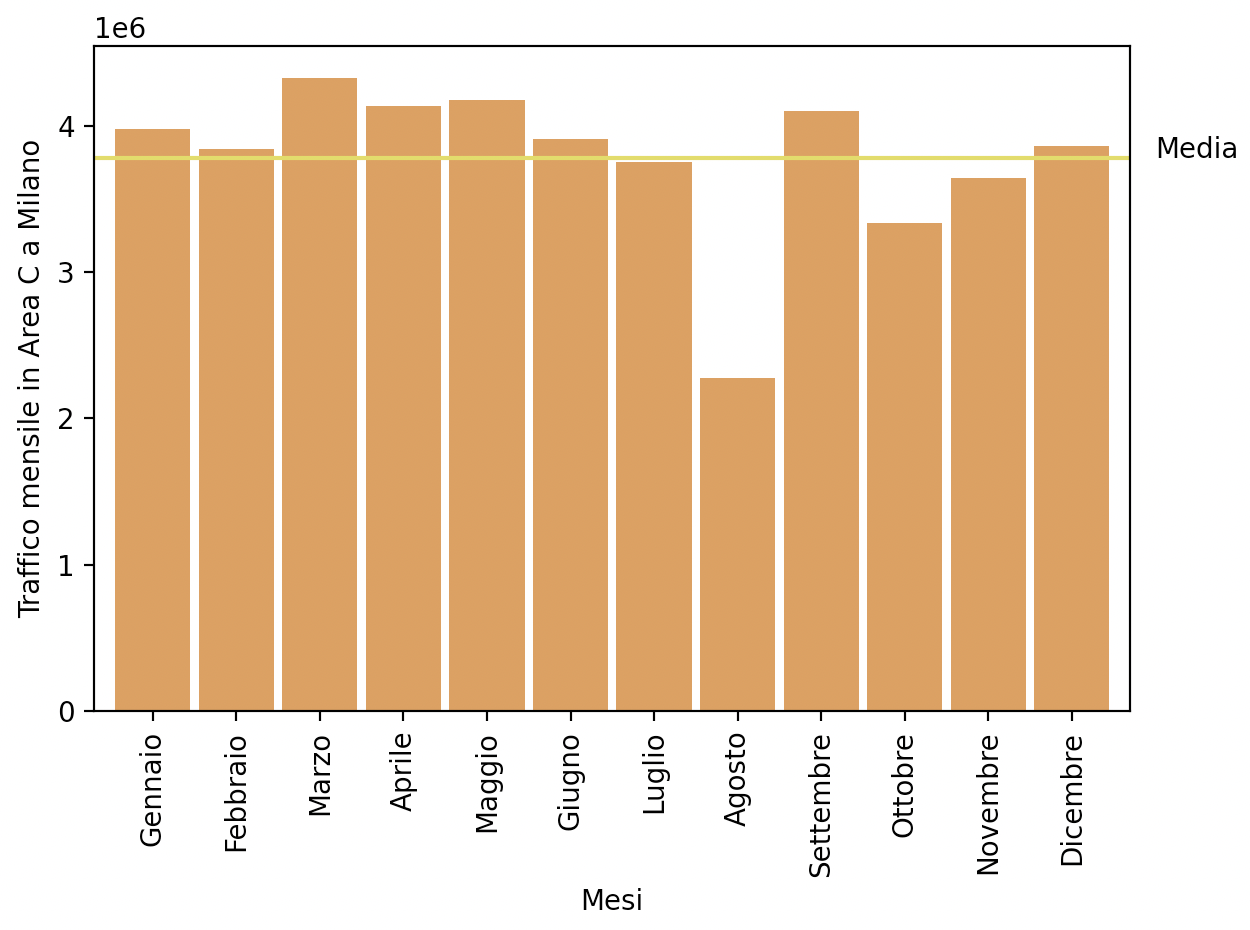
\includegraphics[width=\linewidth]{../src/area_c/stima_traffico_mensile.png}
    \caption{Stima del traffico a Milano per mese, tramite accessi all'area C}
    \label{fig:stima-traffico-mensile}
\end{figure}

Una volta ottenuta una stima del traffico per mese, è possibile applicare questa misurazione 
al numero di incidenti mensili.

\begin{figure}
    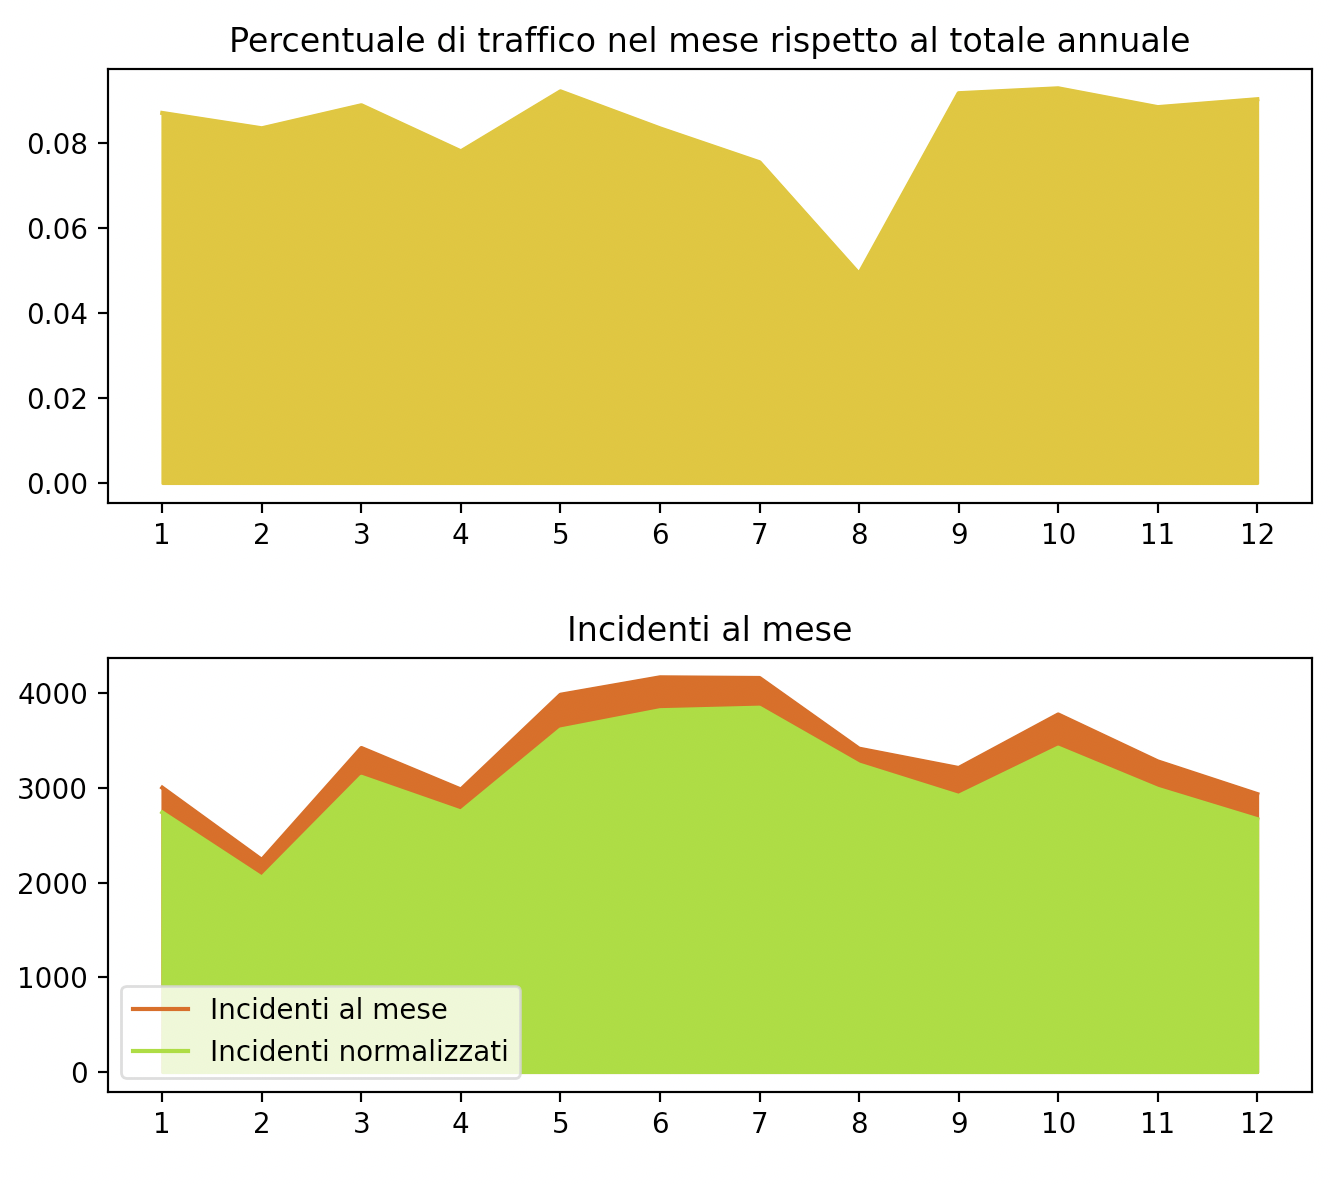
\includegraphics[width=\linewidth]{../src/area_c/incidenti_traffico_mese.png}
    \caption{Incidenti al mese, tenendo conto del traffico nello stesso periodo (2012)}
    \label{fig:incidenti-traffico-mese}
\end{figure}

L'immagine \ref{fig:incidenti-traffico-mese} contiene due grafi, 
il primo riguardante la frazione di traffico annuale che interessa ogni mese; 
mentre il secondo raffigura il numero di incidenti mensili, rispetto al numero di incidenti pesati 
tramite la percentuale di traffico mensile
\footnote{Si è utilizzato l'anno 2012 perchè è il primo anno contenente tutti i dati completi, 
tutti gli altri anni hanno mesi o campi mancanti}.
Dunque, più la curva verde si avvicina alla linea degli incidenti, più il mese ha avuto sinstri 
non direttamente dovuti al traffico.
In particolare si nota che, in Agosto, nonostante un ampia discesa degli accessi all'area C, 
il numero di incidenti siano rimasti alti, e le due linee sono vicine.
D'altra parte, per Maggio e Giugno, le linee si separano per il concetto inverso.

%\clearpage
\subsection{In località di mare gli incidenti aumentano in estate?}

Dalla figura \ref{fig:mesi-estivi} si nota che le province con maggiore incidentalità 
cambiano in Agosto rispetto a tutto l'anno. In particolare, ad aumentare in volume sono le 
province di Brescia e Palermo.

\begin{figure}
    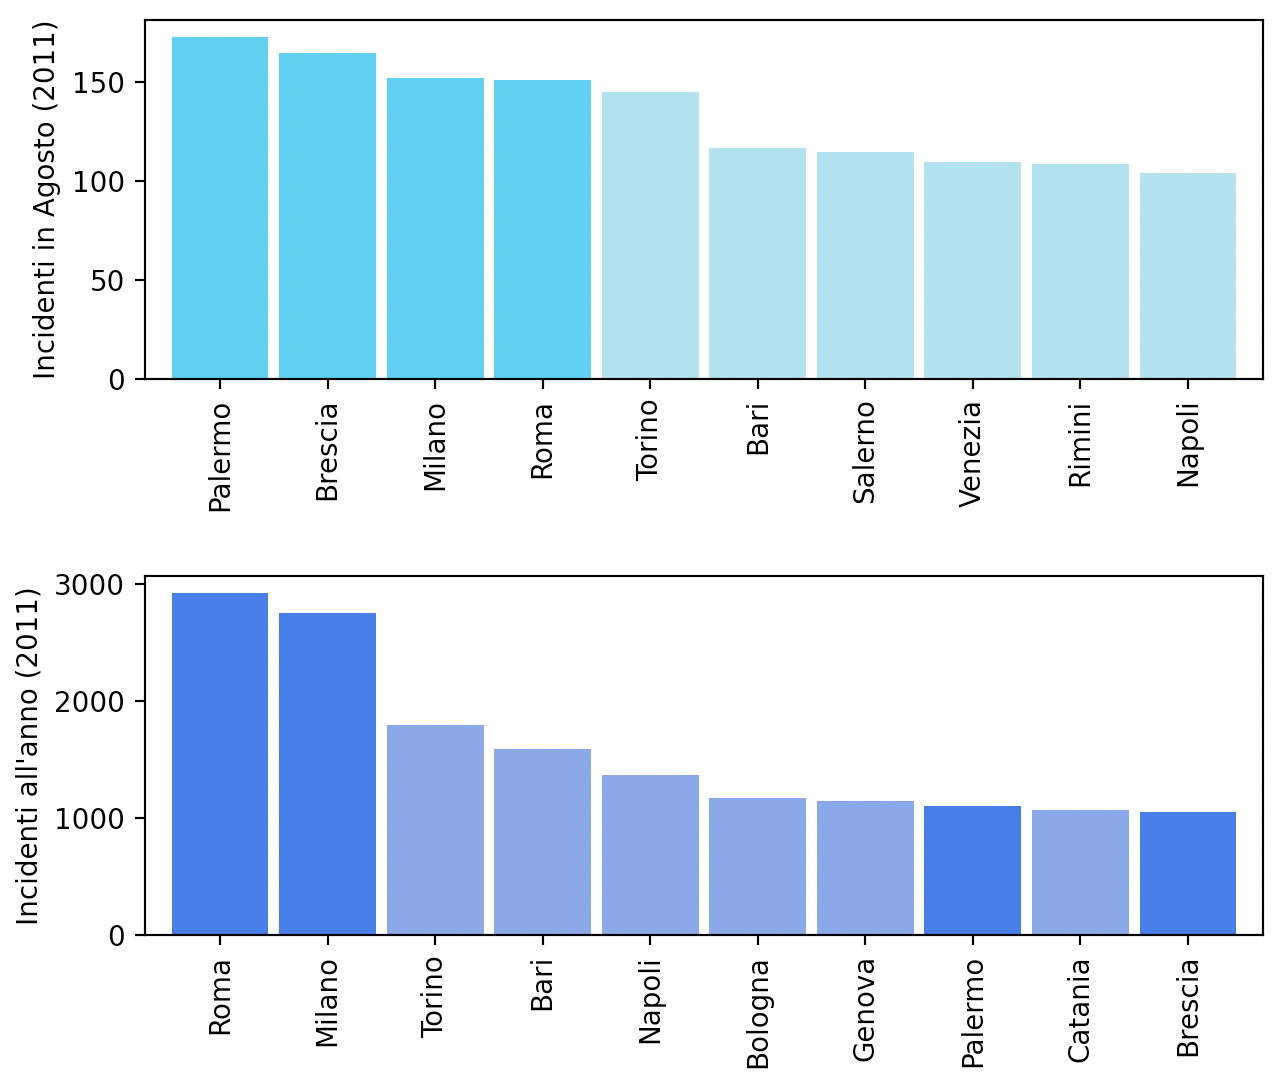
\includegraphics[width=\linewidth]{../src/incidenti/incidenti_senza_coords/mese_incidenti/mesi_estivi.png}
    \caption{Prime 10 province per incidenti in Agosto rispetto a tutto l'anno}
    \label{fig:mesi-estivi}
\end{figure}

Tuttavia questo comportamento è unico dell'anno 2011, in quanto, per gli altri due anni in cui 
si dispone dei dati sui mesi, 2012 e 2013, Milano e Roma hanno il primato di 
incidenti sia per l'anno che per il mese di Agosto individuale.

\todo{lelepado: metto i grafi degli altri due anni?}


\begin{figure}
    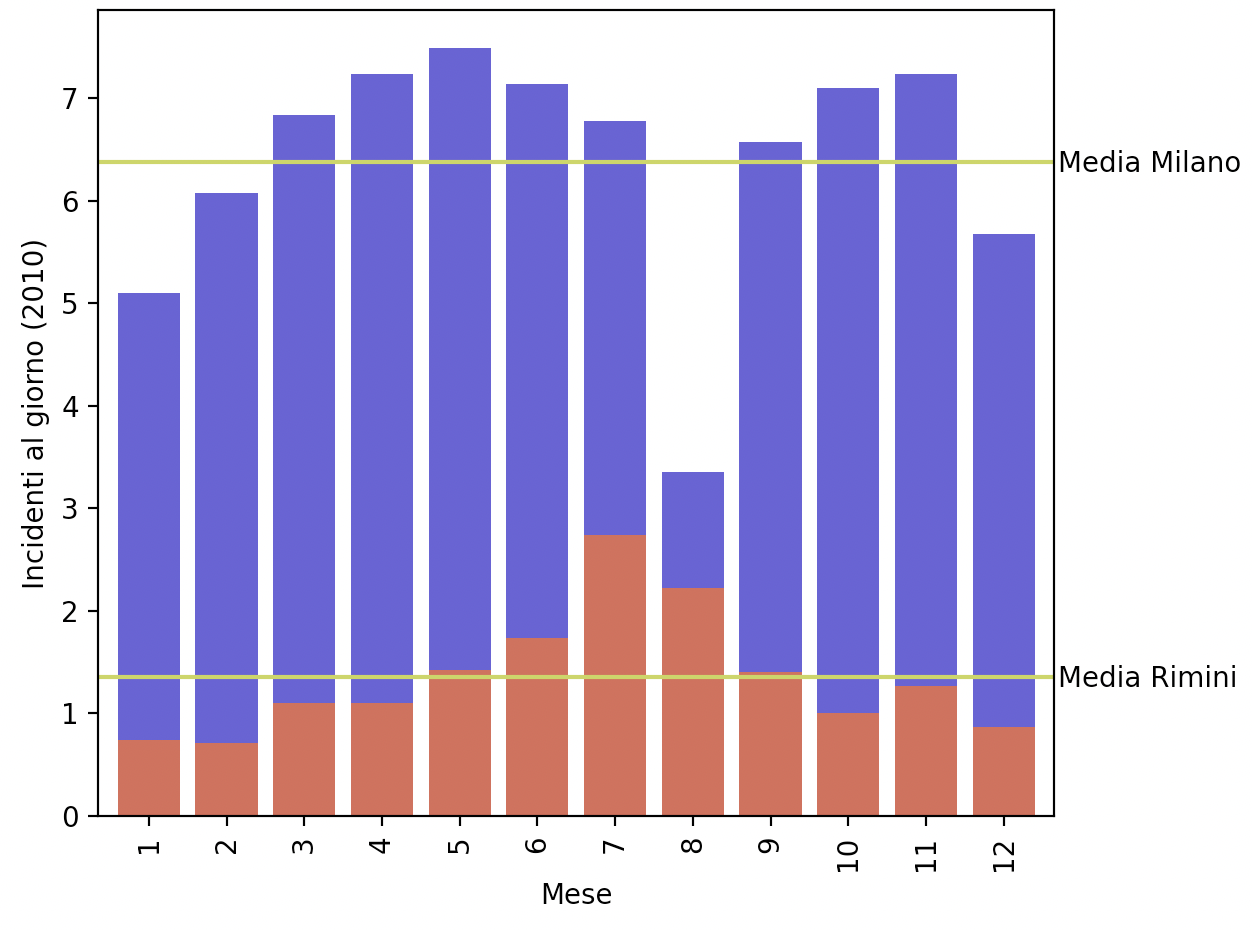
\includegraphics[width=\linewidth]{../src/incidenti/incidenti_senza_coords/mese_incidenti/milano_rimini.png}
    \caption{Incidenti per mese a Milano e Rimini}
    \label{fig:milano-rimini}
\end{figure}

\begin{figure}
    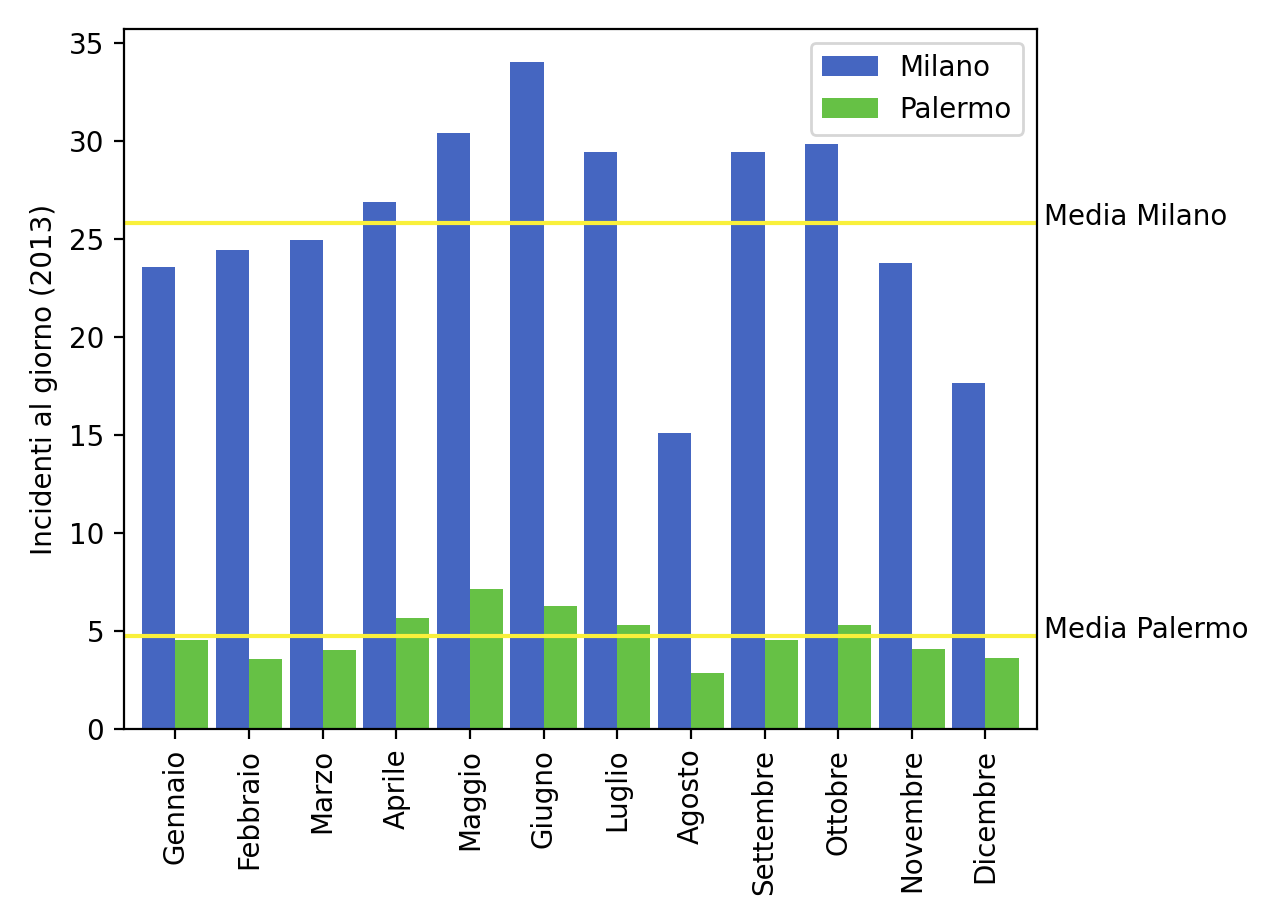
\includegraphics[width=\linewidth]{../src/incidenti/incidenti_senza_coords/mese_incidenti/palermo_milano.png}
    \caption{Incidenti per mese a Milano e Palermo}
    \label{fig:palermo-milano}
\end{figure}

Sono state ricavate alcune località in cui si è riscontrata la tendenza inversa, come in provincia 
di Rimini, raffigurata nel grafo \ref{fig:milano-rimini}.
Lo stesso procedimento si è anche realizzato per Palermo, nella figura \ref{fig:palermo-milano}, 
dove a Luglio e Agosto, il numero di incidenti supera addirittura il volume di Milano.

Nella seguente tabella, sono indicati gli incrementi per anno del numero di incidenti a Rimini.
L'incremento constante per ogni anno, conferma che questo fenomeno è un trend annuale.

\begin{center}
    \def\arraystretch{1.5}%  
    \begin{tabular}{ |c|c|c| } 
    \hline
    Anno & Agosto & Luglio \\ 
    \hline
    \rowcolor{TableGray}
    2010 & 63.75\% & 101.72\% \\ 
    2011 & 60.49\% & 54.6 \%  \\
    \rowcolor{TableGray}
    2012 & 45.93\% & 75.97\%  \\
    2013 & 51.82\% & 116.37\% \\
    \hline
    \end{tabular}
\end{center}


Osservando il grafo raffigurante gli incidenti per mese della Valle d'Aosta, 
in figura \ref{fig:aosta}, 
è possibile notare un notevole incremento di incidenti sia in Gennaio che in Agosto, possibili 
conseguenze, rispettivamente, dell'inizio della stagione sciistica ed estiva.

\begin{figure}
    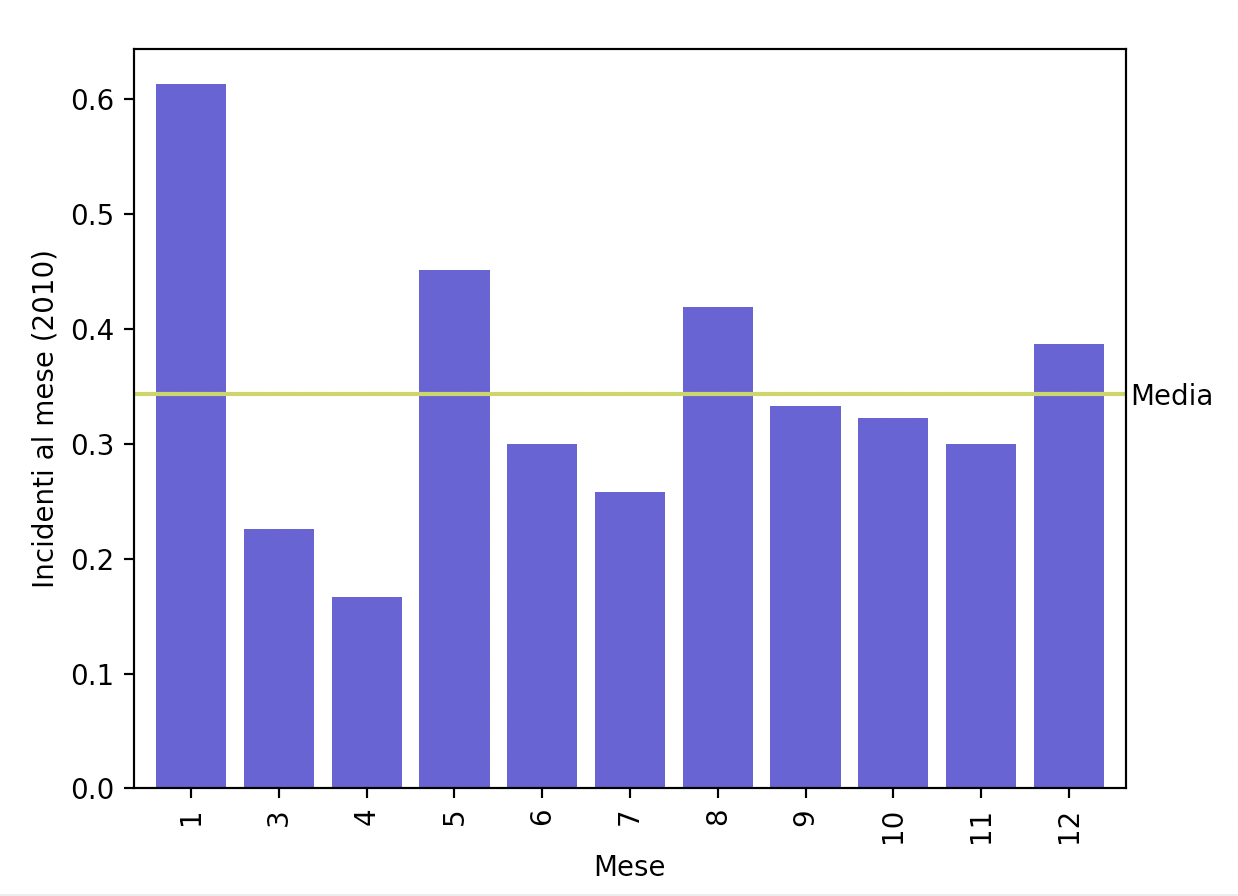
\includegraphics[width=\linewidth]{../src/incidenti/incidenti_senza_coords/mese_incidenti/aosta_mese.png}
    \caption{Incidenti per mese Valle d'Aosta}
    \label{fig:aosta}
\end{figure}

Questa tendenza avviene ogni anno?

\begin{center}
    \def\arraystretch{1.5}%  
    \begin{tabular}{ |c|c|c| } 
    \hline
    Anno & Agosto & Gennaio \\ 
    \hline
    \rowcolor{TableGray}
    2010 & -2.93 \% & 78.48\%  \\ 
    2011 & 124.0 \% & -32.12\% \\
    \rowcolor{TableGray}
    2012 & 52.25 \% & -41.44\% \\
    2013 & -15.21\% & -24.63\% \\
    \hline
    \end{tabular}
\end{center}

Il comportamento degli incidenti in Valle d'Aosta, mostrato in figura \ref{fig:aosta-trimestre} 
è molto inconsistente, soprattutto in Agosto.
Va specificato che la taglia del campione con cui si sta lavorando, per questa provincia, 
è molto piccolo, e sicuramente influisce sulle percentuali di incremento e decremento 
degli incidenti.\\
Nonostane ciò, se si assume che Gennaio 2010 sia un outlier, il numero di incidenti in 
questo mese è sempre in decremento, in modo molto consistente, rispetto alla media.

\begin{figure}
    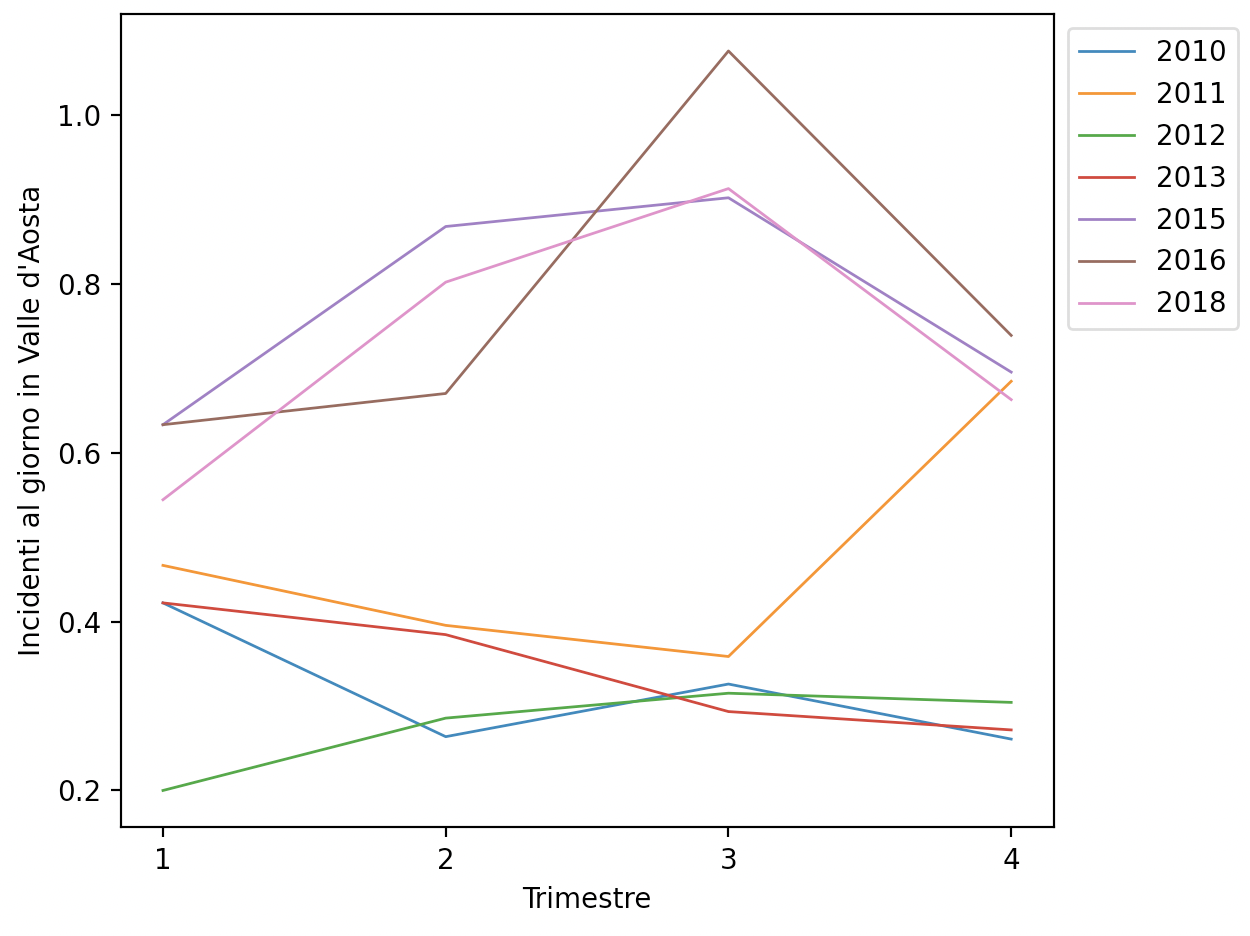
\includegraphics[width=\linewidth]{../src/incidenti/incidenti_senza_coords/mese_incidenti/aosta_timestre.png}
    \caption{Incidenti per trimestre in Valle d'Aosta}
    \label{fig:aosta-trimestre}
\end{figure}

La prima cosa che è possibile notare nel grafo, è che il picco di Gennaio del 2010 è 
in linea con la tendenza del trimestre invernale. 
Tuttavia, si osserva anche che dall'anno 2015 c'è un ampio gap nel numero di incidenti. 
\'E un cambio di metro di misurazione? 

\begin{figure}
    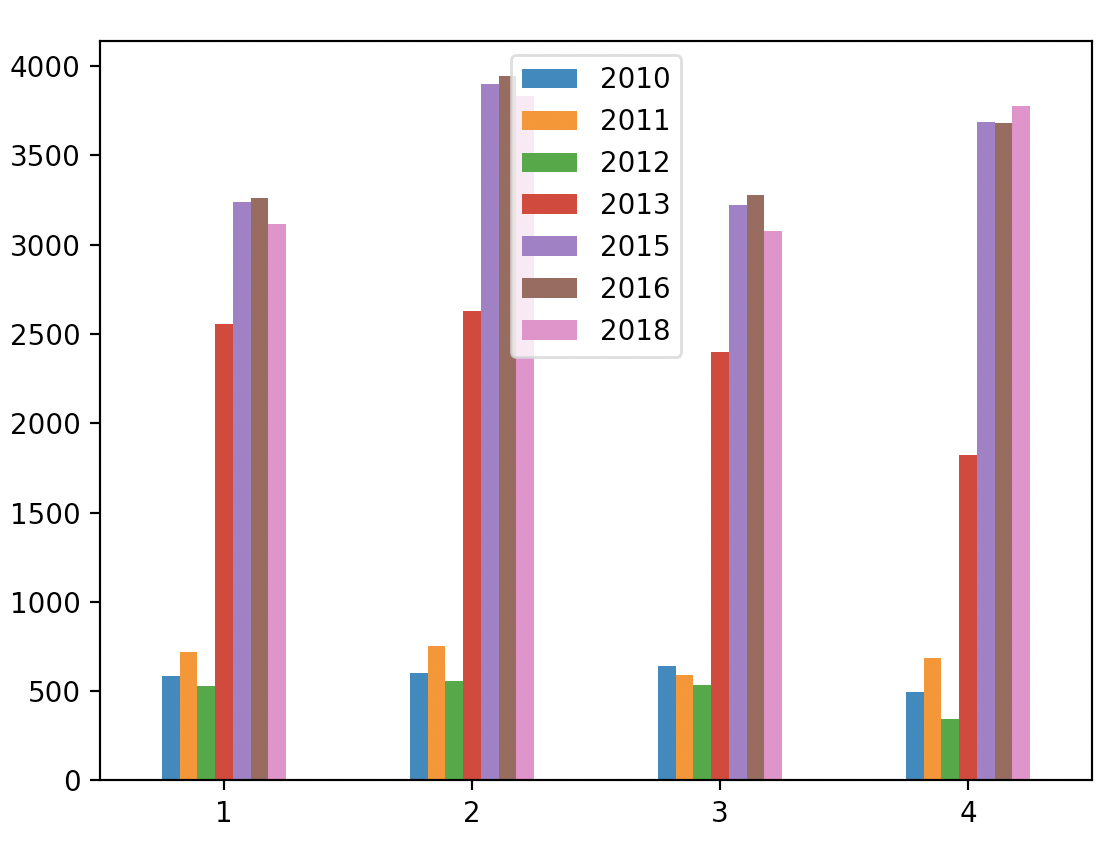
\includegraphics[width=\linewidth]{../src/incidenti/incidenti_senza_coords/mese_incidenti/milano_trimestre.png}
    \caption{Incidenti per trimestre a Milano}
    \label{fig:milano-trimestre}
\end{figure}

\begin{figure}
    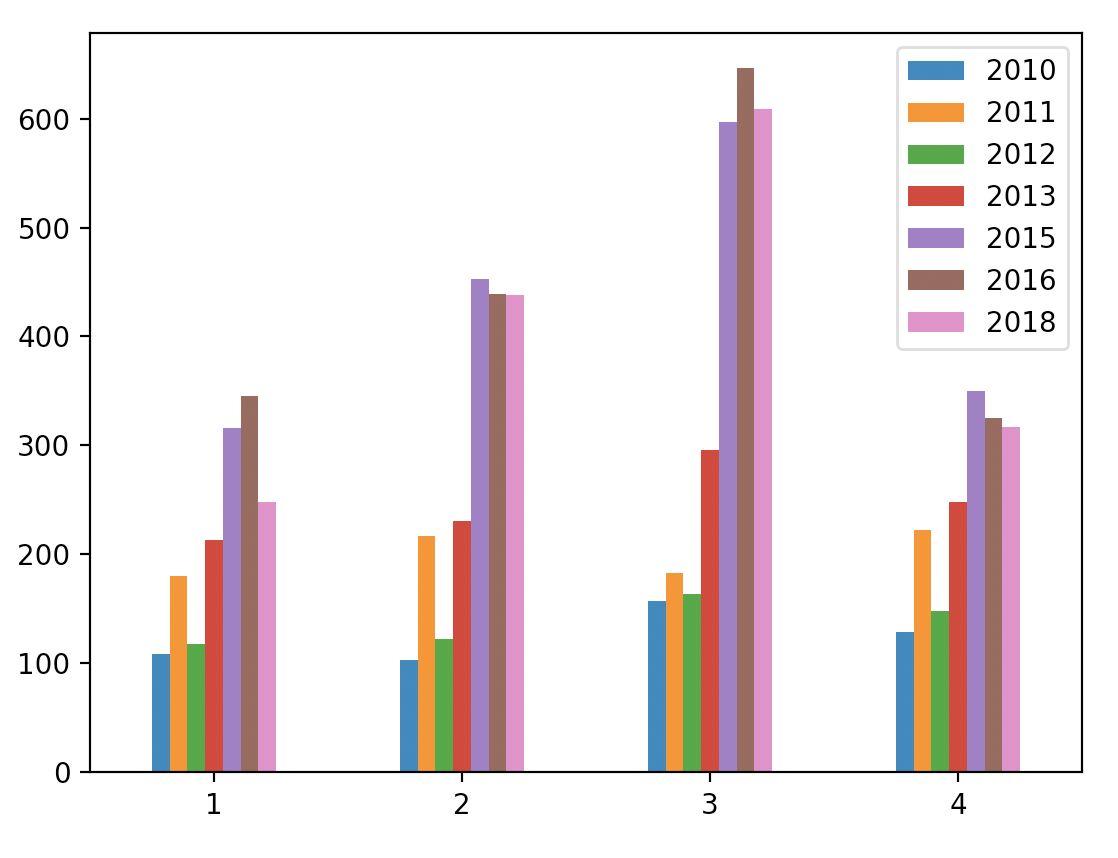
\includegraphics[width=\linewidth]{../src/incidenti/incidenti_senza_coords/mese_incidenti/rimini_trimestre.png}
    \caption{Incidenti per trimestre a Rimini}
    \label{fig:rimini-trimestre}
\end{figure}

I grafi equivalenti di Milano e Rimini, nelle figure 
\ref{fig:milano-trimestre} e \ref{fig:rimini-trimestre} rispettivamente, 
mostrano la stessa tendenza di incremento del numero 
di incidenti, che è possibile vedere nella figura \ref{fig:incremento-incidenti}, 
di cui si è parlato in un precedente capitolo.

%\clearpage
\section{Dati Istat su tipi di incidenti e incroci}

%\clearpage
\subsection{Le tipologie di incidenti più frequenti}

\begin{figure}
    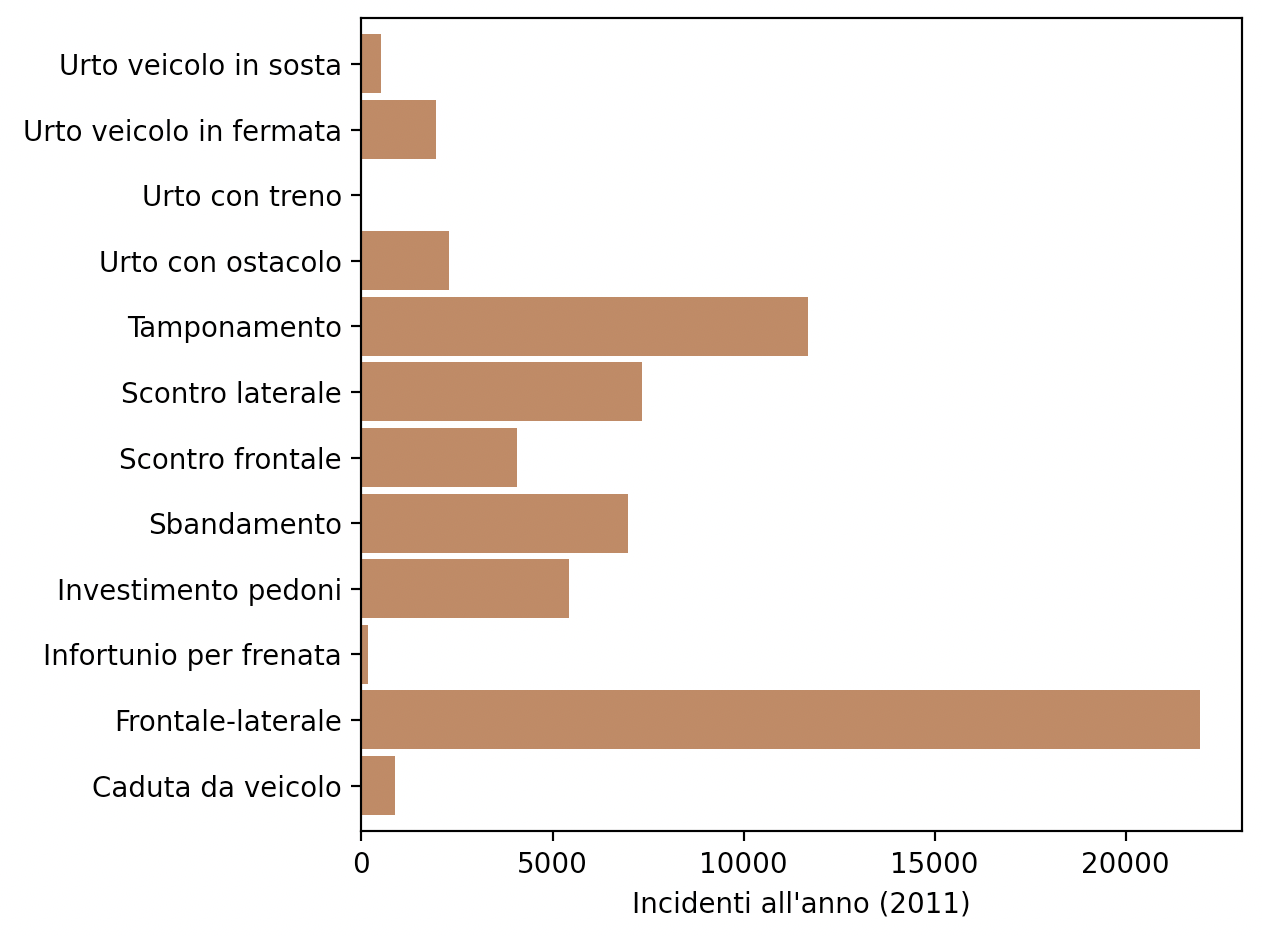
\includegraphics[width=\linewidth]{../src/incidenti/incidenti_senza_coords/localizzazione_incidente/tipo_incidente.png}
    \caption{Tipologia di incidente}
    \label{fig:tipo-incidente}
\end{figure}

Nella figura \ref{fig:tipo-incidente} è possibile osservare quali sono gli incidenti più frequenti in un 
anno, in questo caso nel 2018.
In particolare sono molto frequenti scontri frontali, laterali e tamponamenti. 
Gli incidenti frontali-laterali sono i più rappresentati probabilmente per l'ampiezza della 
categoria.

%\clearpage
\subsection{Gli incroci più pericolosi}

Dal grafo \ref{fig:tipo-intersezioni}, 
si nota che la maggior parte degli incidenti avviene nei rettilinei e negli incroci.\\
Per rendere questa affermazione più attendibile, 
bisognerebbe conoscere il numero totale di rettilinei, e di incroci di ogni altro tipo, in 
modo da mettere in relazione i dati assoluti del grafo. 
D'altro canto i risultati trovati sono plausibili, in quanto spesso le automobili raggiungono 
velocità più alta nei rettilinei rispetto a qualsiasi altro tipo di incrocio.

\begin{figure}
    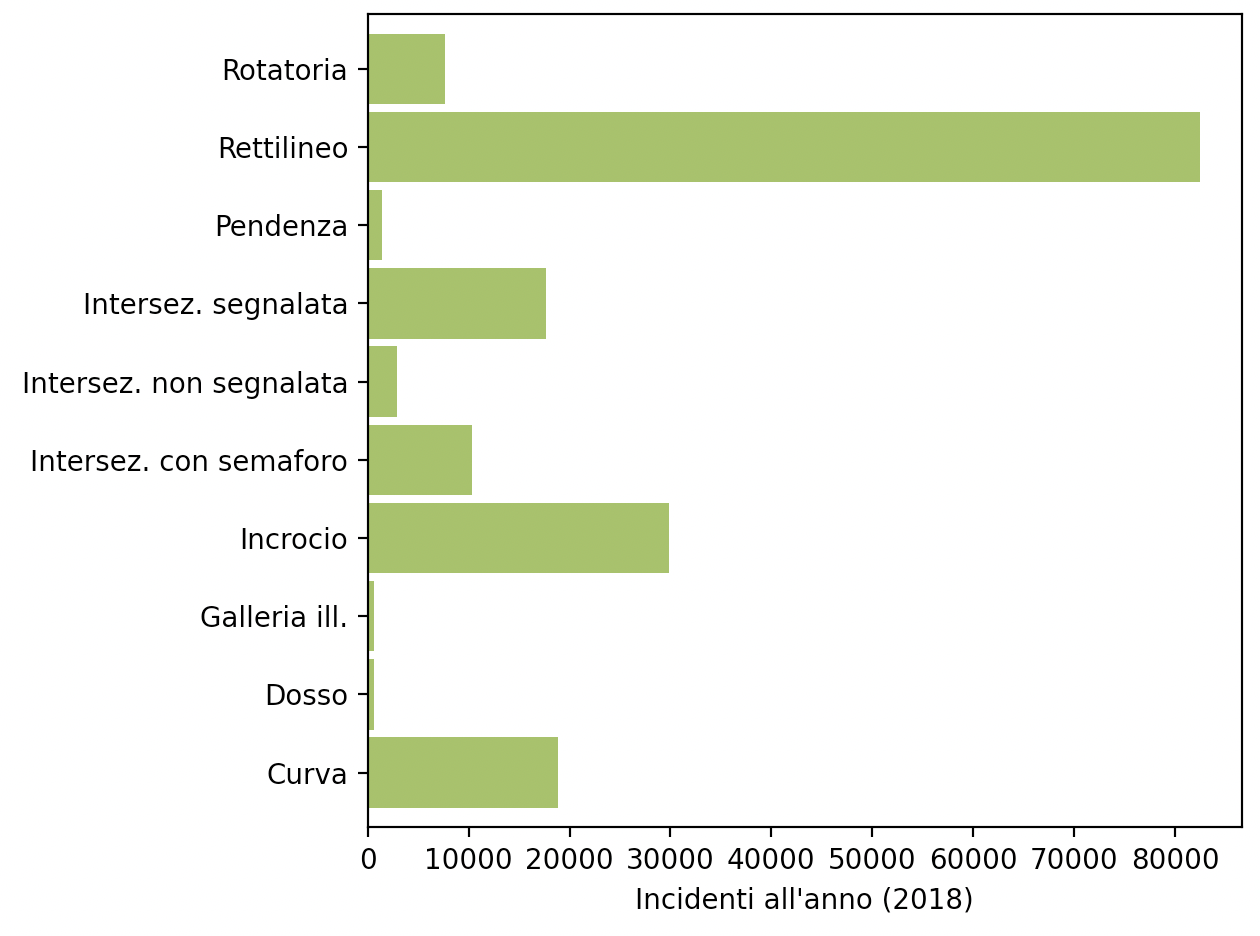
\includegraphics[width=0.5\linewidth]{../src/incidenti/incidenti_senza_coords/localizzazione_incidente/intersezioni.png}
    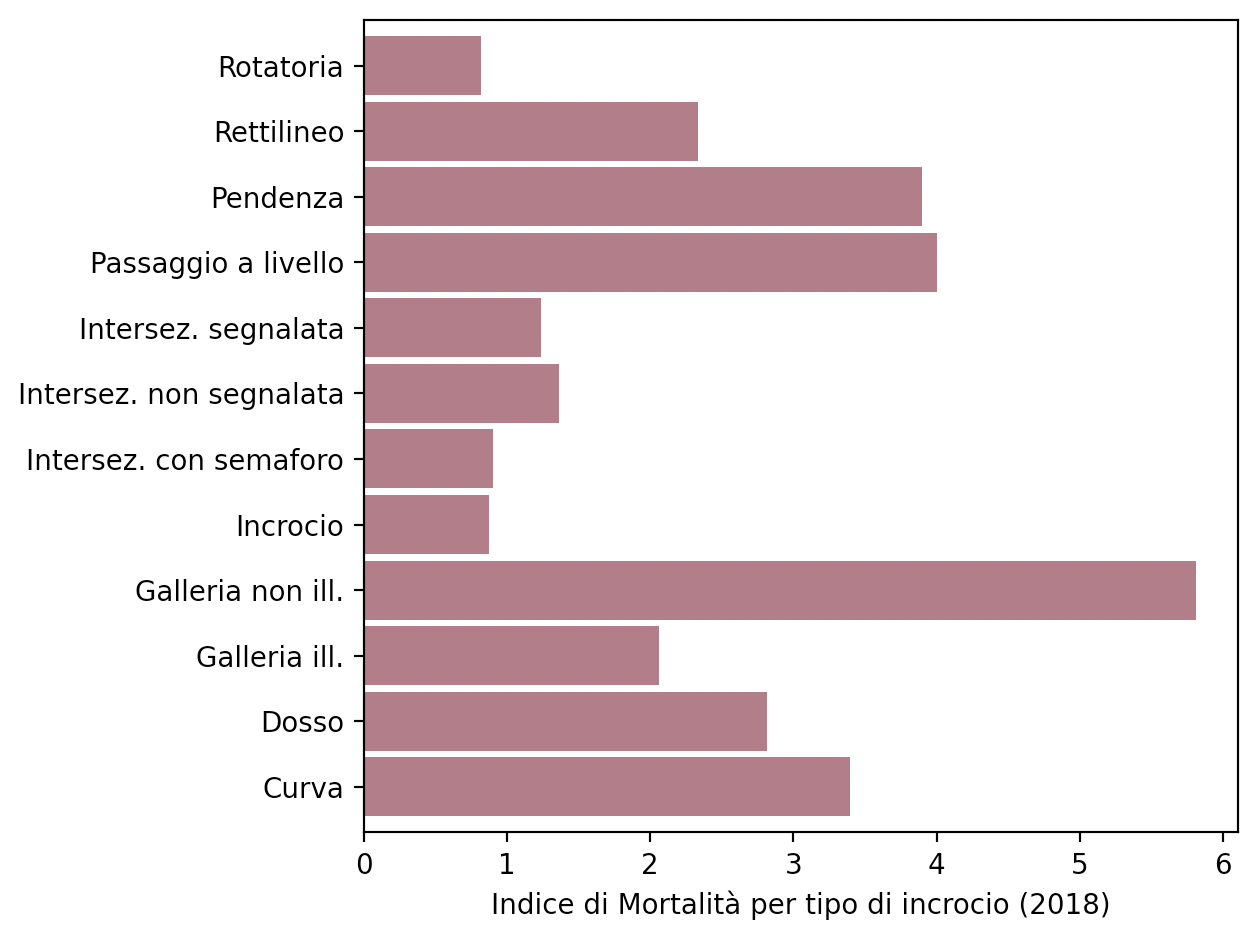
\includegraphics[width=0.5\linewidth]{../src/incidenti/incidenti_senza_coords/localizzazione_incidente/indice_mortalita.png}
    \caption{Percentuale di incidenti e rispettivo indice di mortalità per tipo di incrocio}
    \label{fig:tipo-intersezioni}
\end{figure}


\begin{lstlisting}
    incroci = 'intersezione_o_non_interse3'
    
    df = {}
    for inc in data[incroci].unique(): 
        df[inc] = 0

    for inc, morti in zip(data[incroci], data['morti']): 
        df[inc] += morti

    indice_mortalita = pd.Series(df.values(),index =  df.keys()).sort_index()

    num_incroci = data[incroci].value_counts().sort_index()

    mortalita = pd.DataFrame([indice_mortalita * 100 / num_incroci], 
        index=['indice']
    ).transpose()
\end{lstlisting}


\begin{center}
    \def\arraystretch{1.5}%  
    \begin{tabular}{ |c|c|c| } 
    \hline
    Tipo di Incrocio & Indice di Mortalità & Indice di Feriti \\ 
    \hline
    \rowcolor{TableGray}
    Incrocio                & 0.88 & 143.10 \\
    Rotatoria               & 0.82 & 127.22 \\
    \rowcolor{TableGray}
    Intersez. segnalata     & 1.24 & 142.14 \\
    Intersez. con semaforo  & 0.9 & 147.05 \\
    \rowcolor{TableGray}
    Intersez. non segnalata & 1.36 & 139.97\\
    Passaggio a livello     & 4.0 & 134.67\\
    \rowcolor{TableGray}
    Rettilineo              & 2.33 & 138.94\\
    Curva                   & 3.39 & 145.26\\
    \rowcolor{TableGray}
    Dosso                   & 2.82 & 156.49\\
    Pendenza                & 3.9 & 134.10\\
    \rowcolor{TableGray}
    Galleria ill.           & 2.06 & 165.87\\
    Galleria non ill.       & 5.81 & 132.59\\
    \hline
    \end{tabular}
\end{center}


%\clearpage
\subsection{Le tipologie di incidenti che provocano più feriti}

\begin{figure}
    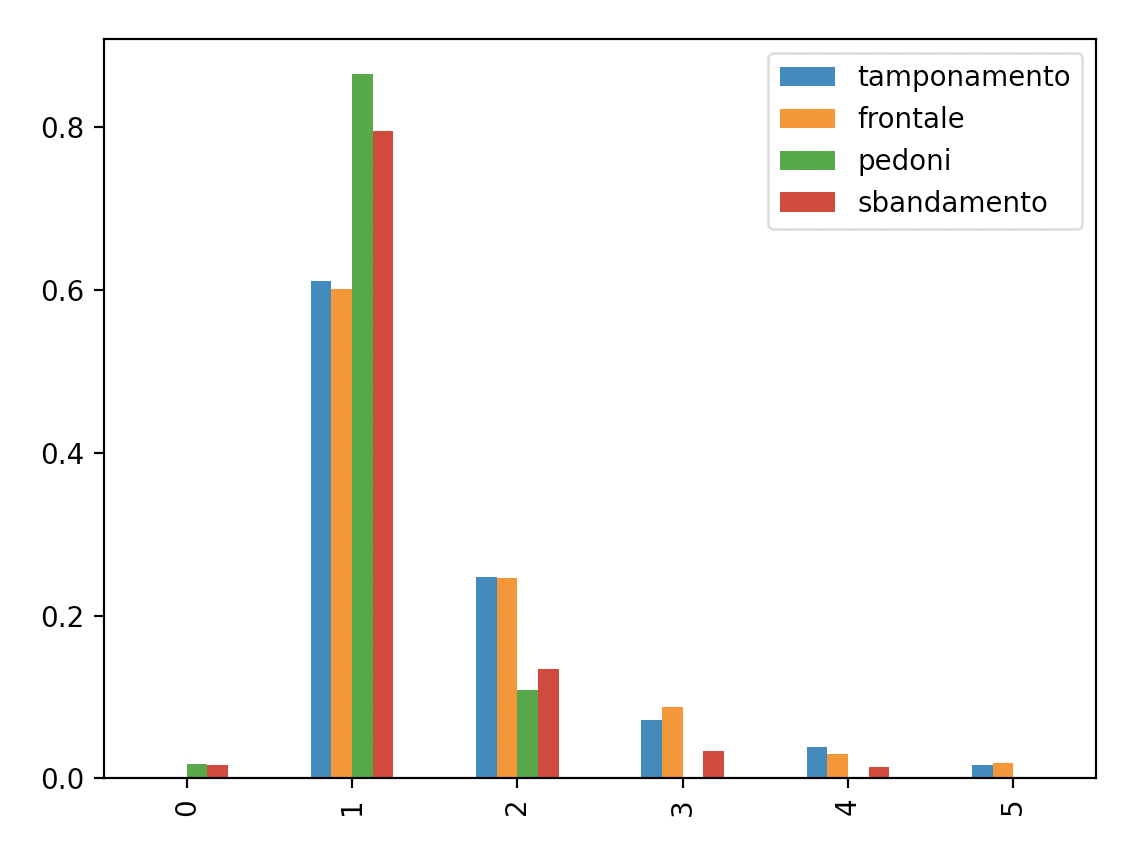
\includegraphics[width=\linewidth]{../src/incidenti/incidenti_senza_coords/natura_incidente/numero_feriti.png}
    \caption{Numero di feriti in base alla natura dell'incidente}
    \label{fig:numero-feriti}
\end{figure}

Nella figura \ref{fig:numero-feriti} si nota che esistono tipologie di sinistri che 
favoriscono la presenza di un solo ferito, come gli incidenti con pedone. 
Al contrario, incidenti come il tamponamento e frontale, 
hanno una più alta percentuale di situazioni con due o più feriti.

%\clearpage
\subsection{Incroci che favoriscono incidenti con pedoni}

La figura \ref{fig:pedoni-intersezioni} mostra il numero di incidenti con pedoni coinvolti, 
ordinati in base alla tipologia di intersezioni e al numero di persone coinvolte.

\begin{figure}
    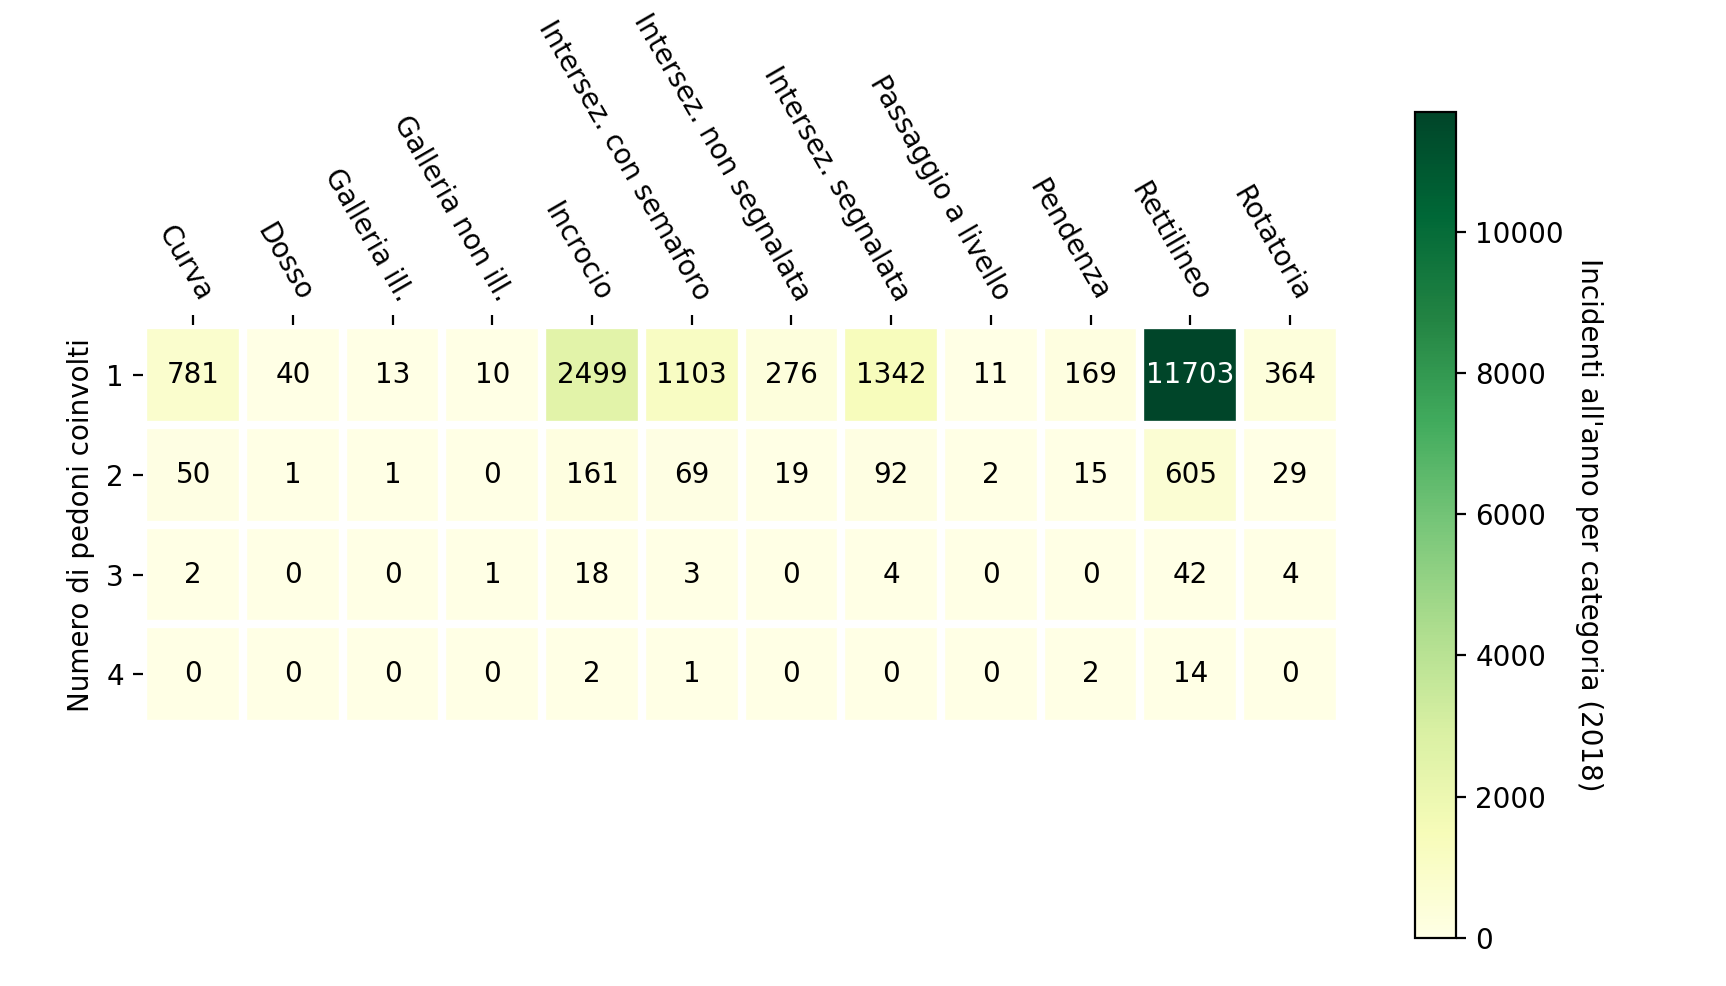
\includegraphics[width=\linewidth]{../src/incidenti/incidenti_senza_coords/pedoni/pedoni_incroci.png}
    \caption{Tipologia di intersezioni e pedoni coinvolti}
    \label{fig:pedoni-intersezioni}
\end{figure}

Come nel grafo \ref{fig:tipo-intersezioni} spicca che 
tra i tipi di strada che favoriscono incidenti con pedoni spiccano i rettilinei, 
probabilmente in parte per l'alta velocità dei veicoli, ma anche per l'alto volume di
tratti di strada di questo tipo.

%\clearpage
\subsection{Età dei pedoni coinvolti in incidenti}

\begin{figure}
    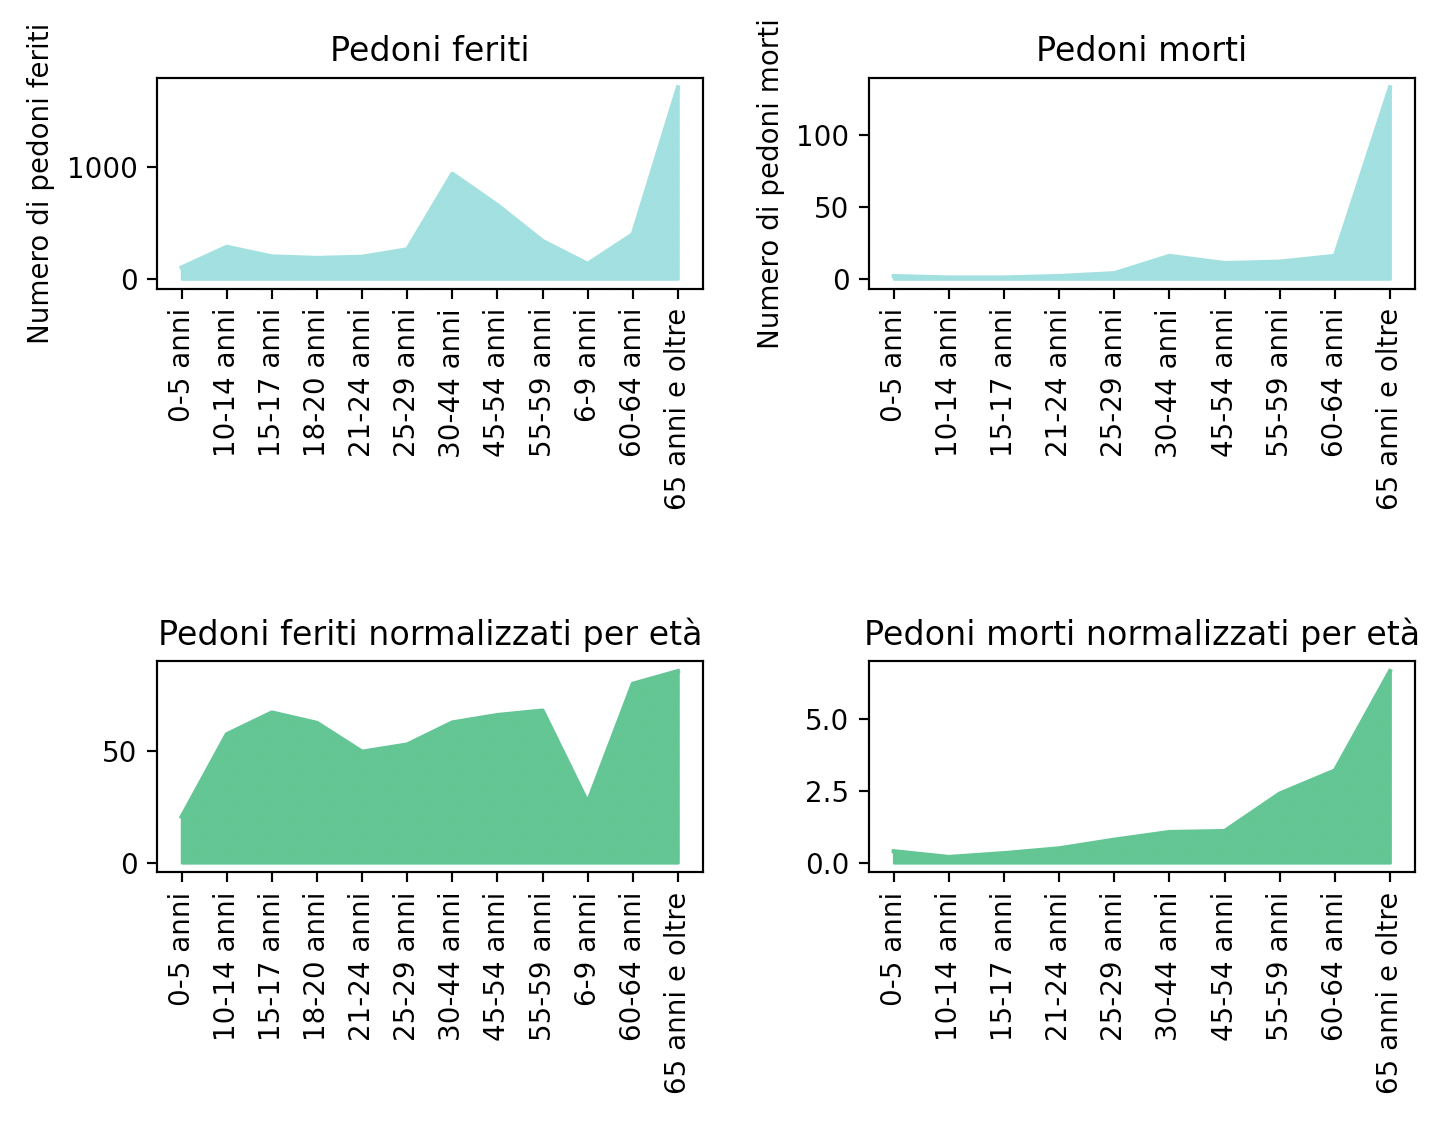
\includegraphics[width=\linewidth]{../src/incidenti/incidenti_senza_coords/pedoni/eta_pedoni.png}
    \caption{Fasce di età dei pedoni coinvolti in incidenti}
    \label{fig:eta-pedoni}
\end{figure}

Dal grafo \ref{fig:eta-pedoni} si osserva che la fascia di età più colpita dagli 
incidenti è quella dei 65 anni, va comunque detto che questo gruppo probabilmente 
contiene la maggior parte degli individui.
Se si normalizza per anni contenuti in ogni fascia, ipotizzando un numero
costante di persone di ogni età, si ottiene un grafo, per quanto riguarda i pedoni 
feriti, molto differente. \\
La normalizzazione tiene conto che la fascia di età '65 anni e oltre' vale venti anni.

\begin{lstlisting}[language=Python]
    anni_per_fascia_feriti = pd.Series([5,5,3,3,4,5,15,10,5,5,5,20,1])
    anni_per_fascia_morti = pd.Series([5,5,3,4,5,15,10,5,5,20,1])
    
    pedoni_feriti = pedoni_feriti.values / np.array(anni_per_fascia_feriti)
    pedoni_morti = pedoni_morti.values / np.array(anni_per_fascia_morti)
\end{lstlisting}

Tuttavia, non è detto che in Italia il numero di individui con la stessa età sia costante.
Infatti le percentuali di individui per fascia sono
\footnote{\url{https://www.tuttitalia.it/statistiche/popolazione-eta-sesso-stato-civile-2019/}}: 

\begin{center}
    \def\arraystretch{1.5}%  
    \begin{tabular}{ |c|c| } 
    \hline
    Fascia & Percentuale Popolazione \\ 
    \hline
    \rowcolor{TableGray}
    0-5     & 3.9 \% \\ 
    6-9     & 4.5 \% \\
    \rowcolor{TableGray}
    10-14   & 4.8 \% \\
    15-17   & 3.1 \% \\
    \rowcolor{TableGray}
    18-20   & 2.8 \% \\ 
    21-24   & 4   \% \\
    \rowcolor{TableGray}
    25-29   & 5.3 \% \\
    30-44   & 19  \% \\
    \rowcolor{TableGray}
    45-54   & 18.2\% \\ 
    55-59   & 7.3 \% \\
    \rowcolor{TableGray}
    60-64   & 6.4 \% \\
    65$+$   & 19.3\% \\
    \hline
    \end{tabular}
\end{center}

\begin{lstlisting}
    popolazione_std_feriti = [3.9 ,4.5 ,4.8 ,3.1 ,2.8 ,4 ,5.3 ,19,16.2,7.3 ,6.4 ,19.3, 0]
    popolazione_std_morti = [3.9 ,4.8 ,3.1 ,4,5.3 ,19,16.2,7.3 ,6.4 ,19.3, 0]

    pedoni_feriti_vals = pedoni_feriti.values / np.array(popolazione_std_feriti)
    pedoni_morti_vals = pedoni_morti.values / np.array(popolazione_std_morti)
\end{lstlisting}

\begin{figure}
    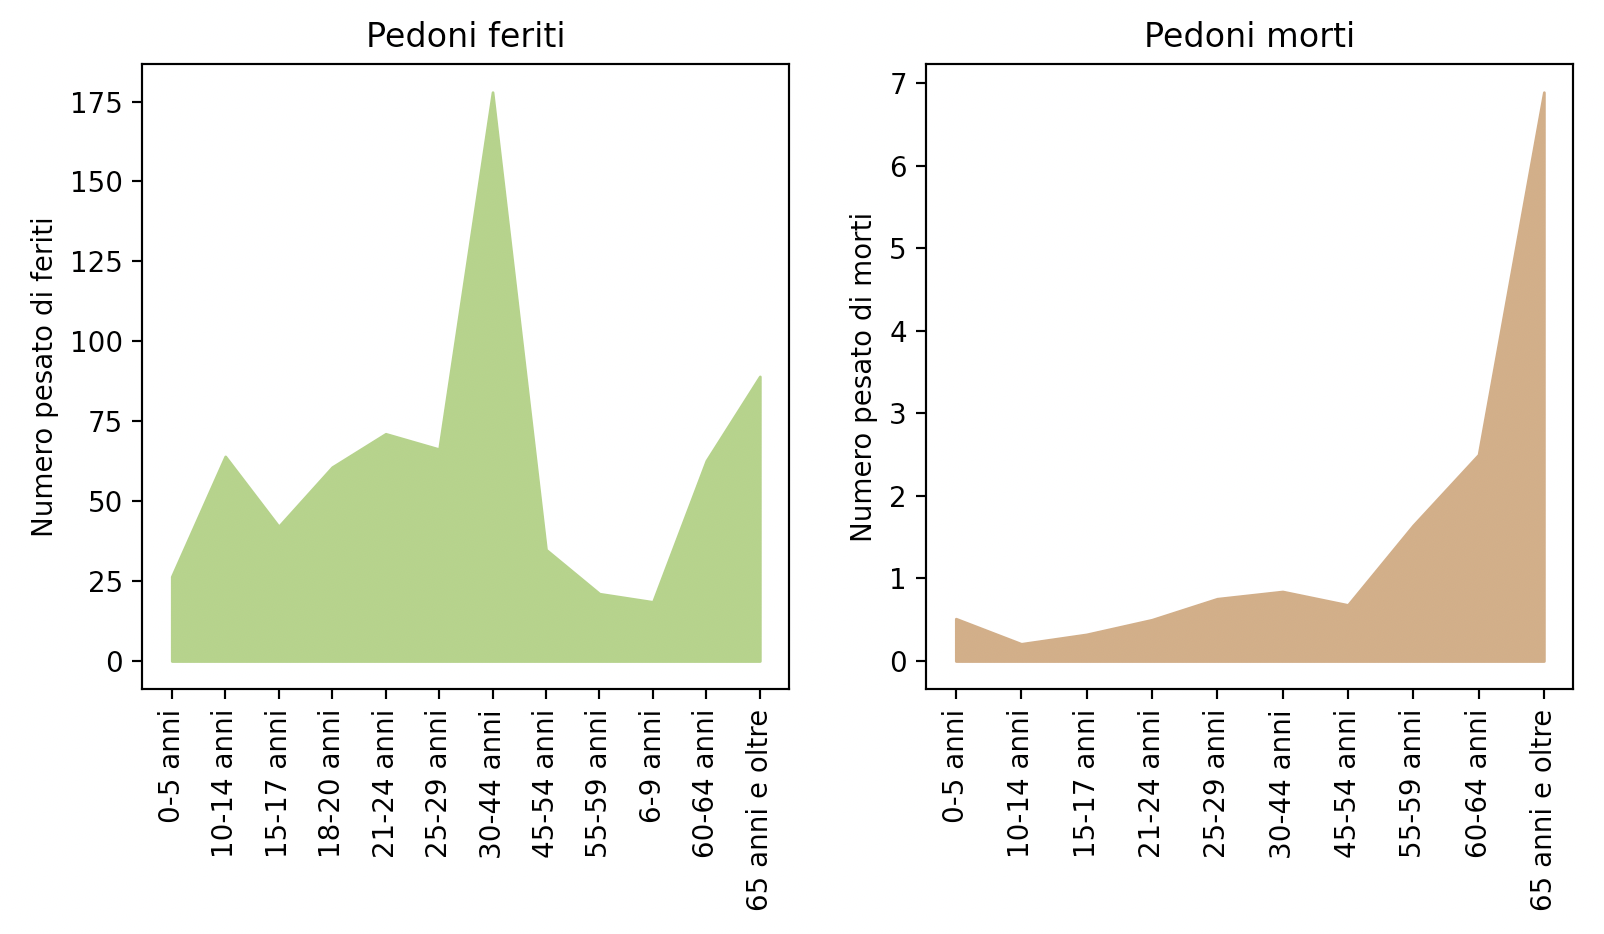
\includegraphics[width=\linewidth]{../src/incidenti/incidenti_senza_coords/pedoni/eta_pedoni_norm.png}
    \caption{Fasce di età dei pedoni coinvolti in incidenti, normalizzate tramite percentuale di popolazione}
    \label{fig:eta-pedoni-norm}
\end{figure}

Una volta aver corretto l'immagine precendente, si ottiene la figura \ref{fig:eta-pedoni-norm} dove, 
soprattutto nel grafo di destra, è presente una curva particolarmente alta nelle fasce più anziane.
Anche nel grafo dei feriti è presente la stessa curva, ma per il volume di persone, la fascia 
dei 30-44 anni, che contiene quattordici anni di età invece che cinque, come 
la maggior parte delle altre fasce, è molto più alta.

L'incremento di feriti nelle fasce più anziane, si può speculare sia dovuto al fatto che 
questi ultimi sono più propensi all'essere feriti in un incidente. 
Tuttavia, è anche possibile che uno dei fattori maggiormente influenti sia il volume di 
pedoni in queste fasce di età.

%\clearpage
\section{Dati ACI}


\subsection{Incidenti per regione}

Grazie al dataset geojson di Guglielmo Celata\footnote{\url{https://github.com/openpolis/geojson-italy}}, 
è stato possibile realizzare le mappe in figura \ref{fig:incidenti-per-regione}, 
che raffigurano rispettivamente, le regioni con più incidentalità nel per ogni anno nelle 
strade provinciali e nelle autostrade, nell'anno 2018.
Ovviamente il nord Italia ha il primato per quanto riguarda gli incidenti, soprattutto nelle regioni 
di Lombardia, Veneto e Emilia Romagna. 
Spicca poi il Lazio, dove la maggior parte degli incidenti avvengono su autostrade, in quanto il volume 
di incidenti è nella media nella prima mappa in figura \ref{fig:incidenti-per-regione}, mentre è il massimo annuale nella 
seconda mappa.

\begin{figure}
    \includegraphics[width=0.5\linewidth]{../src/incidenti/incidenti_aci/mappe_regioni/incidenti_per_regione.png}
    \includegraphics[width=0.5\linewidth]{../src/incidenti/incidenti_aci/mappe_regioni/incidenti_regione_autostrade.png}
    \caption{Incidenti su autostrade e su strade provinciali nel 2018}
    \label{fig:incidenti-per-regione}
\end{figure}

Per quanto riguarda, invece, il numero di incidenti per ogni anno, 
dalla heatmap \ref{fig:regione-heatmap} 
si nota che non cambia molto di anno in anno, e le regioni con maggiore numero di incidenti rimangono 
sempre Lombardia e Veneto.

\begin{figure}
    \includegraphics[width=\linewidth]{../src/incidenti/incidenti_aci/mappe_regioni/regioni_heatmap.png}
    \caption{Incidenti all'anno per regione su strade provinciali}
    \label{fig:regione-heatmap}
\end{figure}

Se invece si guardasse la differenza tra mesi estivi e mesi invernali?

\begin{figure}
    \includegraphics[width=\linewidth]{../src/incidenti/incidenti_aci/mappe_regioni/incidenti_estate_inverno.png}
    \caption{Incidenti per regione nei mesi di Gennaio e Agosto}
    \label{fig:incidenti-estate-inverno}
\end{figure}

Il grafo \ref{fig:incidenti-estate-inverno} mostra che, per alcune regioni, la differenza del  
numero di incidenti tra Agosto e Gennaio è molto ampia, come per Trentino, Emilia, Veneto e Friuli.
In figura \ref{fig:incidenti-per-mese}, si osserva che la maggior parte degli incidenti, 
per quanto riguarda le autostrade, avvengono tra Luglio e Agosto, dunque è corretto che,  
nella maggior parte delle regioni, il volume di sinistri per quest'ultimo sia maggiore rispetto a Gennaio. 

I grafi precedenti, soprattutto le heatmap regionali, non tengono conto del volume del traffico.
Non avendo informazioni riguardanti il traffico in tutta Italia, si sono stimate queste informazioni 
tramite il numero di patentati per regione.
Una stima eseguita con il numero di patentati per regione, non è molto accurato, 
in quanto molte persone patentate in una regione, possono lavorare in altre e dunque influire 
in modo errato al conteggio degli incidenti. 

\begin{figure}
    \includegraphics[width=\linewidth]{../src/incidenti/incidenti_aci/mappe_regioni/incidenti_patenti.png}
    \caption{Incidenti e patentati per regione}
    \label{fig:incidenti-patentati}
\end{figure}

Se si visualizza il rapporto tra incidenti e patentati per regione (figura \ref{fig:incidenti-patentati}), 
si osserva una chiara distinzione tra nord, centro e sud Italia.
A cosa è dovuta questa ampia disparità?
Nella seguente tabella sono riportate le medie di incidenti annuali per regione, 
e quella di patentati per regione.

\begin{center}
    \def\arraystretch{1.5}%  
    \begin{tabular}{ |c|c|c| } 
    \hline
    Zona & Media di Incidenti annuali & Patentati (in Milioni) \\ 
    \hline
    \rowcolor{TableGray}
    Nord    &   2470 &   2,28 \\ 
    Centro  &   2395 &   1,97 \\ 
    \rowcolor{TableGray}
    Sud     &   1145 &   1,57 \\ 
    \hline
    \end{tabular}
\end{center}

Il grafo \ref{fig:incidenti-patentati-bar} è stato suddiviso tra regioni del nord, centro e sud, per facilitare 
la lettura, e indica le percentuali di incidenti e patentati per la rispettiva regione. 
\'E subito osservabile che, nella maggior parte delle regioni del centro, la percentuale di incidenti 
supera quella di patentati, mentre nel sud Italia accade il fenomeno opposto.

\begin{figure}
    \includegraphics[width=\linewidth]{../src/incidenti/incidenti_aci/mappe_regioni/incidenti_patenti_bar.png}
    \caption{Incidenti e patentati per regione}
    \label{fig:incidenti-patentati-bar}
\end{figure}

\begin{figure}
    \includegraphics[width=\linewidth]{../src/incidenti/incidenti_aci/mappe_regioni/incidenti_patenti_box.png}
    \caption{Incidenti e patentati per nord, centro e sud Italia}
    \label{fig:incidenti-patentati-box}
\end{figure}

La figura \ref{fig:incidenti-patentati-box} permette di capire il motivo della disparità 
tra centro e sud Italia, perchè il numero di incidenti al sud è molto minore, mentre 
non c'è un'ampia differenza di patentati. 

Quali potrebbero essere le motivazioni di questa disparità?
Come già accennato in precendenza, una delle motivazioni principali 
deve essere la destinazione lavorativa della popolazione.


%\clearpage
\subsection{Le strade pericolose in provincia di Milano}

\begin{figure}
    \includegraphics[width=\linewidth]{../src/incidenti/incidenti_aci/autostrade/incidenti_line_chart.png}
    \caption{Autostrade con più incidenti nel 2012}
    \label{fig:line-incidenti-milano}
\end{figure}

Per realizzare la figura \ref{fig:line-incidenti-milano}, sono state prese in considerazione alcune 
tra le autostrade e strade statali più trafficate e si è segnata la posizione approssimata.

\begin{lstlisting}
    strade = gp.read_file("dataset/incidenti/aci/autostrade/posizione_autostrade.geojson").to_crs(epsg=3857)
    strade.index = strade['name']

    strade = gp.GeoDataFrame(incidenti[ore], geometry=strade['geometry'])
    ax = strade.plot(markersize=strade[ore].sum() * 10, alpha=0.5)
\end{lstlisting}


\subsection{Incidenti per provincia}

\begin{figure}
    \includegraphics[width=0.5\linewidth]{../src/provincia/lombardia_autostrade.png}
    \includegraphics[width=0.5\linewidth]{../src/provincia/lombardia_strade_prov.png}
    \caption{Incidenti nelle autostrade e nelle strade provinciali in Lombardia}
    \label{fig:lombardia-strade}
\end{figure}

Nella figura \ref{fig:lombardia-strade} sono mostrati gli incidenti in Lombardia, 
avvenuti rispettivamente nelle autostrade e nelle strade provinciali, divisi per provincia.
In entrambi i casi, si nota che la provincia di Milano è quella più caratterizzata da incidenti. 
D'altra parte, per quanto riguarda le differenze, nelle province di Bergamo e Como il numero di 
incidenti cresce molto nelle strade provinciali rispetto alle autostrade.

\begin{figure}
    \includegraphics[width=0.5\linewidth]{../src/provincia/lazio_autostrade.png}
    \includegraphics[width=0.5\linewidth]{../src/provincia/lazio_strade_prov.png}
    \caption{Incidenti nelle autostrade e nelle strade provinciali nel Lazio}
    \label{fig:lazio-strade}
\end{figure}

Invece, nella figura \ref{fig:lazio-strade} raffigurante il Lazio, 
per quanto nelle autostrade il numero di incidenti sia molto più alto 
rispetto a quello delle strade provinciali, 
non ci sono molte differenze di volume tra le province.

%\clearpage
\subsection{Esiste correlazione tra incidenti e feriti?}

E allo stesso modo, esiste correlazione tra morti e incidenti, o tra morti e feriti?\\
Ovviamente si attende un esito positivo a queste domande.
L'indice di correlazione utilizzato è il coefficiente di Pearson.

\begin{lstlisting}
    data = pd.read_csv("dataset/incidenti/aci/autostrade/comuni_2018.csv")
    inc = data['INC']
    fer = data['FER']
    mor = data['MOR']
\end{lstlisting}

Una volta divisi i dati, è possibile calcolare l'indice tramite il metodo \textit{corr()}, i risultati 
sono riportati nella seguente tabella.

\begin{center}
    \def\arraystretch{1.5}%  
    \begin{tabular}{ |c|c|c| } 
    \hline
    Incidenti & Incidenti & Feriti \\ 
    Feriti & Morti & Morti \\ 
    \hline
    0.9836 & 0.3385 & 0.3355 \\ 
    \hline
    \end{tabular}
\end{center}

Il coefficiente di Pearson, per quanto riguarda Incidenti e Feriti, 
è molto vicino a uno, quindi i due campioni sono strettamente correlati.
I coefficienti riguardanti i morti sono molto meno vicini a uno, probabilmente per il minor numero 
di incidenti mortali, che rendono il campione più ristretto.

\begin{figure}
    \includegraphics[width=\linewidth]{../src/incidenti/incidenti_aci/provincia/corr_incidenti_feriti.png}
    \caption{Correlazione tra numero di feriti e incidenti}
    \label{fig:corr-incidenti-feriti}
\end{figure}

Tracciando il grafo \ref{fig:corr-incidenti-feriti}, dei primi trenta valori del dataset ACI, 
è chiaramente visibile la correlazione tra numero di incidenti e numero di feriti.
L'unico dubbio che possa sorgere è che il numero di feriti sia maggiore del numero di incidenti, 
tuttavia controllando il dataset, ogni riga contiene un numero di feriti maggiore. 

\begin{center}
    \def\arraystretch{1.5}%  
    \begin{tabular}{ |c|c|c|c| } 
    \hline
    Provincia & Comune & Incidenti & Feriti \\ 
    \hline
    \rowcolor{TableGray}
    Torino & Brandizzo & 5 & 10\\
    Torino & Chivasso & 12 & 18\\
    \rowcolor{TableGray}
    Torino & Rondissone & 6 & 12\\
    Torino & Settimo Torinese & 25 & 40\\
    \hline
    \end{tabular}
\end{center}

%\clearpage
\subsection{Le autostrade più pericolose}
\begin{figure}
    \includegraphics[width=\linewidth]{../src/incidenti/incidenti_aci/autostrade/autostrade.png}
    \caption{Autostrade con più incidenti nel 2018}
    \label{fig:incidenti-autostrade}
\end{figure}

Si pu\'o notare subito, dalla figura \ref{fig:incidenti-autostrade} che, nel 2018, le autostrade con 
più incidenti sono anche quelle più trafficate, come l'Autostrada del Sole e l'Adriatica.

Una domanda che sorge spontanea è se le autostrade con più incidenti cambiano al cambiare dell'anno.\\
Un'altra questione potrebbe essere quella delle differenze di incidenti al cambiare dei mesi, 
o dell'orario.\\
Infine ci si potrebbe chiedere se esistono differenze sostanziali, per anno, tra i flussi di 
famiglie che si dirigono in vacanza in Agosto. Per esempio se esistono delle mete 
popolari solo in determinati stagioni, o se i flussi sono equivalenti di anno in anno.


\subsection{Le autostrade più utilizzate cambiano a seconda dell'anno?}

Il numero di persone in vacanza nelle località del centro e sud italia cambiano 
a seconda dell'anno, il numero di incidenti rispecchia questo cambiamento?

\begin{figure}
    \includegraphics[width=\linewidth]{../src/incidenti/incidenti_aci/agosto/autostrade.png}
    \caption{Incidenti in Strade per anno}
    \label{fig:autostrade-anno}
\end{figure}

Controllando le prime cinque strade per incidentalità ogni anno, 
raffigurate nel grafo \ref{fig:autostrade-anno}, si ottiene un'immagine 
abbastanza stabile, in quanto gli itinerari in testa alla classifica sono sempre gli stessi.
Si nota, che la strada statale Adriatica è sempre in prima posizione, 
con una media di $171.5$ incidenti nel mese di Agosto.
Le posizioni successive invece cambiano a seconda dell'anno, in particolare per\'o, l'autostrada 
A4 (Torino-Trieste) ha progressivamente aumentato il numero di incidenti, evento possibilmente 
dovuto all'aumento di popolarita delle vacanze in montagna.

Facendo utilizzo del dataset istat riguardante il turismo in Italia, e in particolare sfruttando 
due indicatori, Tasso di Turisticità
\footnote{Tasso di Turisticità: indica il numero di turisti presenti ogni 100.000 abitanti} 
e turismo in mesi non estivi,
è stato possibile realizzare il grafo \ref{fig:turismo}, contenente questi indici, 
nel periodo a partire dall'anno 1995 fino al 2018.

\begin{figure}
    \includegraphics[width=\linewidth]{../src/turismo/turismo.png}
    \caption{Turismo nelle principali località estive e invernali}
    \label{fig:turismo}
\end{figure}

Ciò che si può concludere, oltre al fatto che le zone di montagna hanno 
un tasso di turisticità particolarmente alto; 
è che, a partire dal 2015, è presente un aumento di turisti nelle località del 
nord Italia, che non è visibile nelle altre regioni.


\subsection{L'incidentalità su autostrade dipende dai mesi dell'anno?}
\begin{figure}
    \includegraphics[width=\linewidth]{../src/incidenti/incidenti_aci/autostrade/mesi_autostrade.png}
    \caption{Incidenti per mese nel 2018}
    \label{fig:incidenti-per-mese}
\end{figure}

Le curve nel grafo \ref{fig:incidenti-per-mese} sono state normalizzate per bilanciare il volume di incidenti maggiori per 
l'autostrada Adriatica.
L'Adriatica e l'Aurelia, autostrade utilizzate molto durante i mesi caldi, hanno un picco di 
incidenti in Luglio e Agosto, mentre l'A1, ha picco più basso in Agosto, probabilmente 
perchè bilanciato dagli incidenti in inverno intorno a Milano.

Se si prendono i dati della A1, si nota che in Agosto, Settembre e Ottobre il numero degli 
incidenti diminuisce.
Invece sull'Adriatica, raffigurata nel grafo \ref{fig:milano-adriatica}, 
prevalgono incidenti in Luglio e Agosto.

\begin{figure}
    \includegraphics[width=\linewidth]{../src/incidenti/incidenti_aci/autostrade/milano_adriatica_2018.png}
    \caption{Incidenti in provincia di Milano (A1) e sull'Adriatica}
    \label{fig:milano-adriatica}
\end{figure}

La tendenza del grafo \ref{fig:milano-adriatica} è visibile anche negli anni precendenti?

\begin{figure}
    \includegraphics[width=0.5\linewidth]{../src/incidenti/incidenti_aci/autostrade/milano_adriatica_2016.png}
    \includegraphics[width=0.5\linewidth]{../src/incidenti/incidenti_aci/autostrade/milano_adriatica_2014.png}
    \caption{Incidenti in provincia di Milano (A1) e sull'Adriatica}
    \label{fig:milano-adriatica_tendenza}
\end{figure}

Nella figura \ref{fig:milano-adriatica_tendenza} è osservabile la stessa tendenza del grafo precedente, 
con gli incidenti nell'adriatica alti in Luglio e Agosto. 

%\clearpage%
\subsection{In quali orari avvengono incidenti sulle autostrade?}

\begin{figure}
    \includegraphics[width=\linewidth]{../src/incidenti/incidenti_aci/autostrade/tangenziali_autostrade.png}
    \caption{Incidenti nelle principali autostrade di Milano}
    \label{fig:tangenziali-autostrade}
\end{figure}

Il grafo \ref{fig:tangenziali-autostrade} conferma per alcune autostrade i picchi di 
incidenti per il traffico durante orari di punta, 
in particolare è molto visibile per la Torino$-$Trieste e per la Tangenziale ovest.

%\clearpage
\subsection{Quali autostrade sono utilizzate di più per viaggiare in Agosto?}

Non è un segreto che, nel mese di agosto, si ha la maggior parte delle partenze per le vacanze per 
gli Italiani. In genere, per quanto riguarda le partenze in macchina, la tendenza è quella di spostarsi verso sud, 
per raggiungere le località balneari.\\
Spesso, ciò risulta in vari bollini rossi e neri per le autostrade. 
Ci sono mode che cambiano in base all'anno, 
che provocano il numero di incienti a cambiare di anno in anno? 

\begin{figure}
    \includegraphics[width=\linewidth]{../src/incidenti/incidenti_aci/agosto/autostrade_anno_agosto.png}
    \caption{Autostrade con più incidenti per anno, in Agosto}
    \label{fig:autostrade-anno-agosto}
\end{figure}

Il grafo \ref{fig:autostrade-anno-agosto} rappresenta in quali autostrade sono avvenuti 
più incidenti in base al mese di Agosto del rispettivo anno.
Non è sorprendente che le autostrade caratterizzate da un alto numero di bollini rossi e neri 
siano anche le più pericolose.
In particolare spiccano la SS16 Adriatica e SS1 Aurelia, non è difficile trovare il motivo 
dell'alto numero di incidenti, 
queste ultime infatti sono Strade Statali molto lunghe e con corsie di marcia non separate, 
per non parlare del fatto che entrambe le strade passano attraverso un alto numero di centri abitati, 


%%%%%%%%%%%%%%%%%%%%%%%%%%%%%%%%%%%%%%%%%%%%%%%%%%%%%%
%\clearpage
\chapter{Dati su Meteo}

\section{Meteo a Milano}

\subsection{Correlazione tra fattori atmosferici e incidentalità}

\begin{figure}
    \includegraphics[width=0.5\linewidth]{../src/meteo/milano/temp_incidenti_2011.png}
    \includegraphics[width=0.5\linewidth]{../src/meteo/milano/temp_incidenti_2013.png}
    \caption{Incidenti, temperature e umidità medi per mese nel 2011 e nel 2013}
    \label{fig:incidenti-temp}
\end{figure}

La figura \ref{fig:incidenti-temp} mostra, partendo dall'alto, il numero di incidenti 
avvenuti per mese, la temperatura media per mese, e infine l'umidità media.
Sono riportati i due anni con, rispettivamente la maggiore e la minore correlazione tra 
incidenti e fattori atmosferici.
Non è stato possibile eseguire la stessa operazione con dati più recenti, per mancanza del 
campo 'mese', convertito in trimestre a partire dal 2014.
Allo stesso modo non è stato possibile eseguire un'analisi più precisa, per mancanza di dati 
riguardanti il giorno del mese, e disponibili solo per il giorno della settimana.

Senza conoscere gli incidenti giorno per giorno, non è possibile avere una stima della 
correlazione tra i diversi indici del meteo e i sinistri.
Il meglio che è possibile realizzare è un calcolo della correlazione per mese e, per 
avere la maggiore quantità di dati possibile, è stato eseguito per tutti gli 
anni disponibili.
I risultati sono riportati nella tabella sottostante: 

\begin{center}
    \def\arraystretch{1.5}%  
    \begin{tabular}{ |c|c|c|c| } 
    \hline
    Anno & Temperatura & Velocità del Vento & Umidità \\ 
    \hline
    \rowcolor{TableGray}
    2010 & 0.768 & 0.585 & -0.626 \\
    2011 & 0.900 & 0.626 & -0.730 \\
    \rowcolor{TableGray}
    2012 & 0.732 & 0.501 & -0.609 \\
    2013 & 0.658 & 0.465 & -0.516 \\
    \hline
    \end{tabular}
\end{center}

Per le annate a disposizione, i dati sono consistenti tra loro, e indicano la presenza di 
correlazione lineare tra temperature e incidenti, mentre si ha correlazione inversa per quanto 
riguarda l'umidità.

Ciò non significa che, per esempio nel 2011, sia stata l'alta temperatura a provocare 
tutti gli incidenti, anzi, è molto più probabile che il fattore con maggiore 
influenza sia proprio il mese, e non la temperatura o l'umidità.
In altre parole, la correlazione tra due fenomeni non ne implica la causa.


\bibliographystyle{plain}
\bibliography{Biblio}

%\addcontentsline{toc}{chapter}{Bibliografia}

\end{document}
